\documentclass{astroedu-lab}

\begin{document}

\pagestyle{plain}

\begin{problem}{\huge Радиотехническая работа 18\\\\Пассивные электрические цепи\\\\Выполнил Жданов Елисей Б01-205}

\section{Оборудование:}

Макетная плата

Набор резисторов различных сопротивлений

Набор конденсаторов различных емкостей

Набор катушек различной индуктивности

Электронный осциллограф на печатной плате

Электронный генератор сигналов на печатной плате

Программное обеспечение Micro-cap

\section{Задание}

\subsection{Интегрирующие и дифференцирующие звенья}

\subsubsection{Теория}

Два возможные варианта построения делителя напряжения
из резистора R и конденсатора C приводят к интегрирующей
и дифференцирующей цепям на рисунке. Свойства обеих цепей
определяются постоянной времени $\tau = RC$ или характерной ча-
стотой $\omega_0 = \frac{1}{RC}$, $f_0 = \frac{1}{2 \pi R C}$.

\newpage

\begin{figure}[!h]
	\centering
	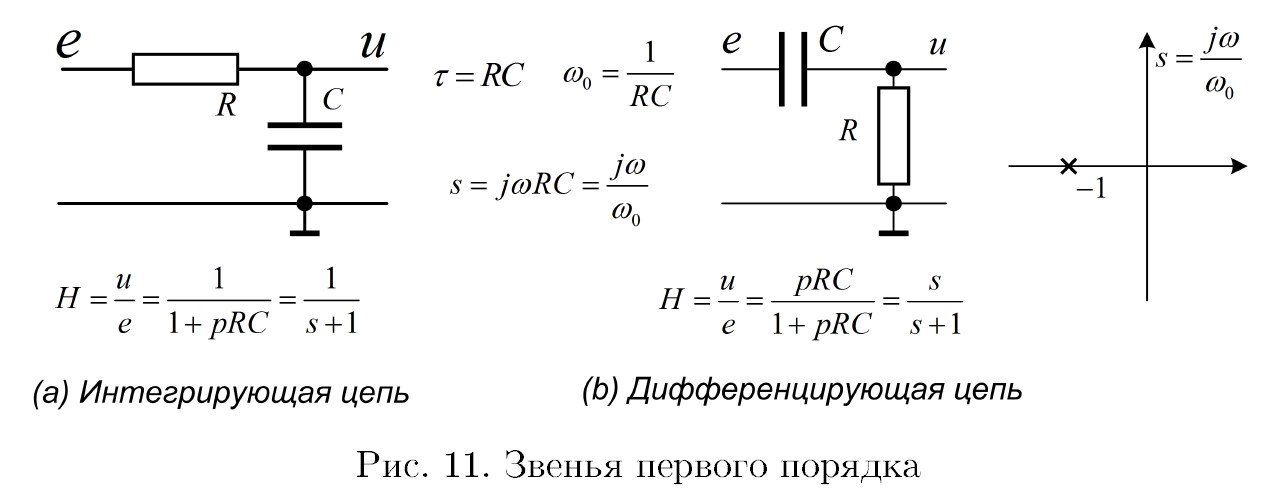
\includegraphics[width=1\textwidth]{1_1.png}
	\label{fig:boiler}
\end{figure}

Присутствие на входе интегрирующей цепи, рис 11a, гармонического напряжения частоты $j \omega = p$ с комплексной амплитудой $e$ вызывает ток с амплитудой $i = \frac{e}{Z} = \frac{e}{R + \frac{1}{p C}}$. Его протекание по емкости C создает выходное напряжение $u = i \frac{1}{p C}$. Для передаточной функции $H(p) = \frac{u}{e}$ получается $H(p) = \frac{1}{1 + p R C}$ или $H(s) = \frac{1}{1 + s}$
. Аналогичным образом, для переда-
точной функции дифференцирующей цепи, рис. 11b, получается
$H(s) = \frac{s}{s+1}$
Оба эти четырехполюсника являются системами первого по-
рядка с единственным полюсом в точке s = -1. Они различают-
ся положениями нулей: нуль дифференцирующей цепи лежит в
нуле при s = 0, а нуль интегрирующей в бесконечности.


Выражение

$$
K(j \omega)=\left.H(s)\right|_{s=\frac{j \omega}{\omega_0}}=\frac{1}{1+j \frac{\omega}{\omega_0}}=\frac{1}{1+j \omega \tau}
$$
для комплексного коэффициента передачи интегрирующей цепи приводит к следующим формулам для ее частотной и фазовой характеристик:
$$
|K(j \omega)|=\frac{1}{\sqrt{1+\left(\frac{\omega}{\omega_0}\right)^2}} ; \quad \varphi(\omega)=\arg K(j \omega)=-\operatorname{arctg}\left(\frac{\omega}{\omega_0}\right) .
$$
Интегрирующая цепь - это фильтр нижних частот (ФНЧ) с полосой пропускания от нуля до граничной частоты $\omega_0=\frac{1}{\tau}$ (частоты среза). На границе полосы пропускания, при $\omega=\omega_0$, $|K(j \omega)|$ снижается с 1 до уровня $\frac{1}{\sqrt{2}} \simeq 0.7=-3 \mathrm{~dB}$.

Лаплас-образ $\frac{H(p)}{p}, H(p)=\frac{\omega_0}{p+\omega_0}$, переходной характеристики интегрирующей цепи $h_0(t)$ факторизуется в сумму элементарных дробей:
$$
L\left[h_0\right](p)=\frac{H(p)}{p}=\frac{1}{p} \frac{\omega_0}{\left(p+\omega_0\right)}=\frac{1}{p}-\frac{1}{p+\omega_0} .
$$
С учетом того, что $\frac{1}{p}=L[\theta(t)], \frac{1}{p+\omega_0}=L\left[e^{-\omega_0 t}\right]$, это дает следующее выражение для $h_0(t)$ :
$$
h_0(t)=\theta(t)-e^{-\omega_0 t}=\theta(t)\left(1-e^{-t / \tau}\right) .
$$
Формулы для АЧХ, ФЧХ и переходной характеристики дифференцирующей цепи получаются по аналогии:
$$
\begin{gathered}
|K(j \omega)|=\frac{\frac{\omega}{\omega_0}}{\sqrt{1+\left(\frac{\omega}{\omega_0}\right)^2}} ; \quad \varphi(\omega)=\arg K(j \omega)=\frac{\pi}{2}-\operatorname{arctg}\left(\frac{\omega}{\omega_0}\right) ; \\
h_0(t)=\theta(t) e^{-\omega_0 t}=\theta(t) e^{-t / \tau} .
\end{gathered}
$$
Дифференцирующая цепь - это фильтр верхних частот (ФВЧ) с полосой пропускания от частоты среза $\omega_0=\frac{1}{\tau}$ до бесконечности. На границе полосы пропускания, при $\omega=\omega_0$,

модуль коэффициента передачи $K(j \omega)$ падает до уровня $\frac{1}{\sqrt{2}} \approx -3$ dB и обращается в нуль при нулевой частоте.

\subsubsection{Выполнение}

1) Соберем схему, удостоверимся в её работоспособности и подключим питание.

В качестве компонент были выбраны резистор $R = 94.64$ Ом, емкость $C = 0.17$ мкФ. Теоретическая постоянная времени состави $\tau = 0.016$ мс.

2) Верхняя граничная частота теоретически составляет $f_0 \approx 9.9 кГц$, на практике же верно $f_0 \approx 10.2$ кГц, что с учетом некоторой погрешности снятия точки совпадает с теорией.

Замеры коэффициента передачи от частоты приведены ниже

\begin{center}
\begin{tabular}{|c|c|}
\hline 
$f_0$, кГц & $K$ \\
\hline
2.6  & 0.58 \\
5.1  & 0.57 \\
10.2 & 0.43 \\
20.4 & 0.25 \\ 
40.8 & 0.14 \\
81.6 & 0.07 \\
163  & 0.04 \\

\hline
\end{tabular}
\end{center}

\newpage

Граф Боде цепи

\begin{figure}[!h]
	\centering
	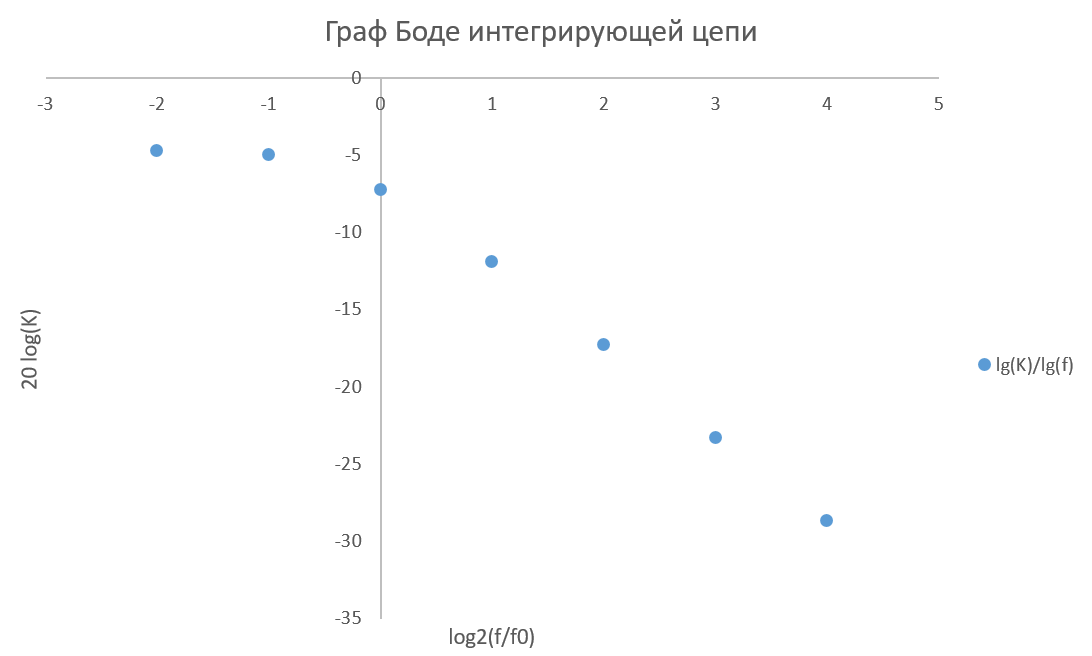
\includegraphics[width=1\textwidth]{1_2.png}
	\label{fig:boiler}
\end{figure}

3) Генератор прямоугольных сигналов показывает время $\tau = 13$ мкс, что в рамках частоты составляет $f_0 = 12.2$ кГц.

4) Проделаем подобные расчеты для интегрирующей цепи

Граничная частота составит $f_0 = 8.47 кГц$.

Замеры коэффициента передачи от частоты приведены ниже

\begin{center}
\begin{tabular}{|c|c|}
\hline 
$f_0$, кГц & $K$ \\
\hline
0.53 & 54.6 \\
1.06 & 87.5 \\
2.12 & 0.43 \\
4.24 & 0.25 \\ 
8.47 & 0.14 \\
16.9 & 0.07 \\
33.9 & 0.04 \\

\hline
\end{tabular}
\end{center}

\newpage

Граф Боде цепи

\begin{figure}[!h]
	\centering
	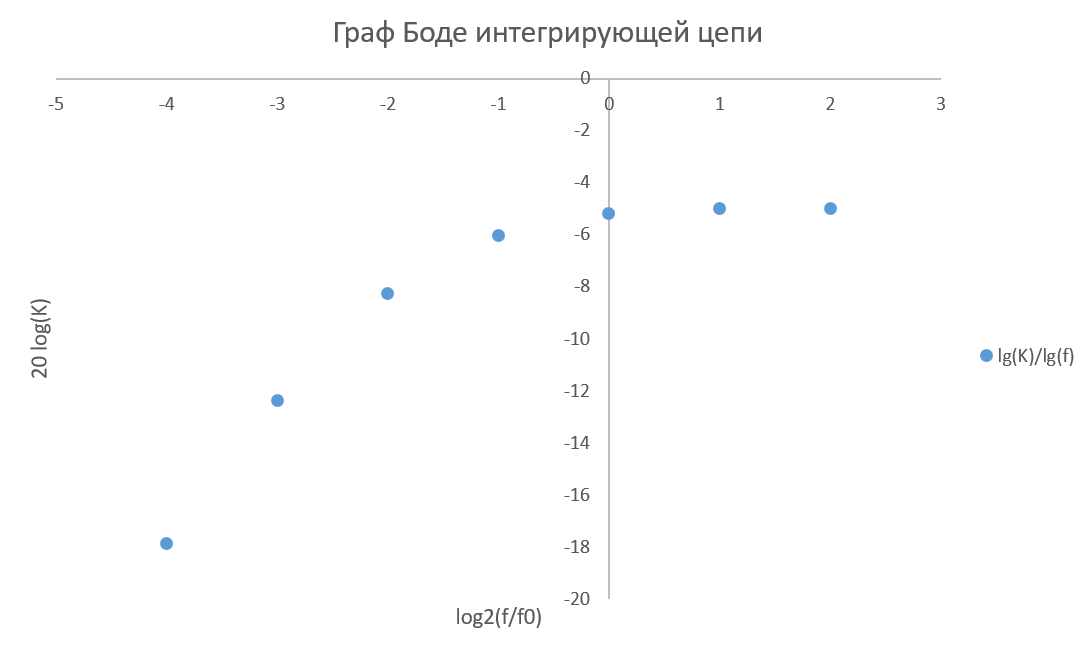
\includegraphics[width=1\textwidth]{1_3.png}
	\label{fig:boiler}
\end{figure}

Генератор прямоугольных сигналов показывает время $\tau = 15$ мкс, что в рамках частоты составляет $f_0 = 10.6$ кГц.

5) Откроем в MicroCap модель rcint.cir. Изучим графики частотной и фазовой характеристики.

\begin{figure}[!h]
	\centering
	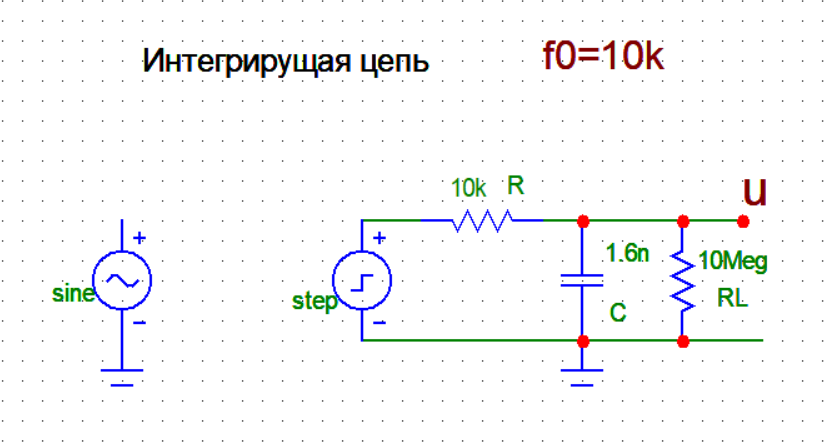
\includegraphics[width=1\textwidth]{1_6.png}
	\label{fig:boiler}
\end{figure}

По графику видно, что передаточная функция цепи для R = 10 кОм принимает вид; $f_0(10 \text{кОм}) = 20 \text{ кГц}$

\begin{figure}[!h]
	\centering
	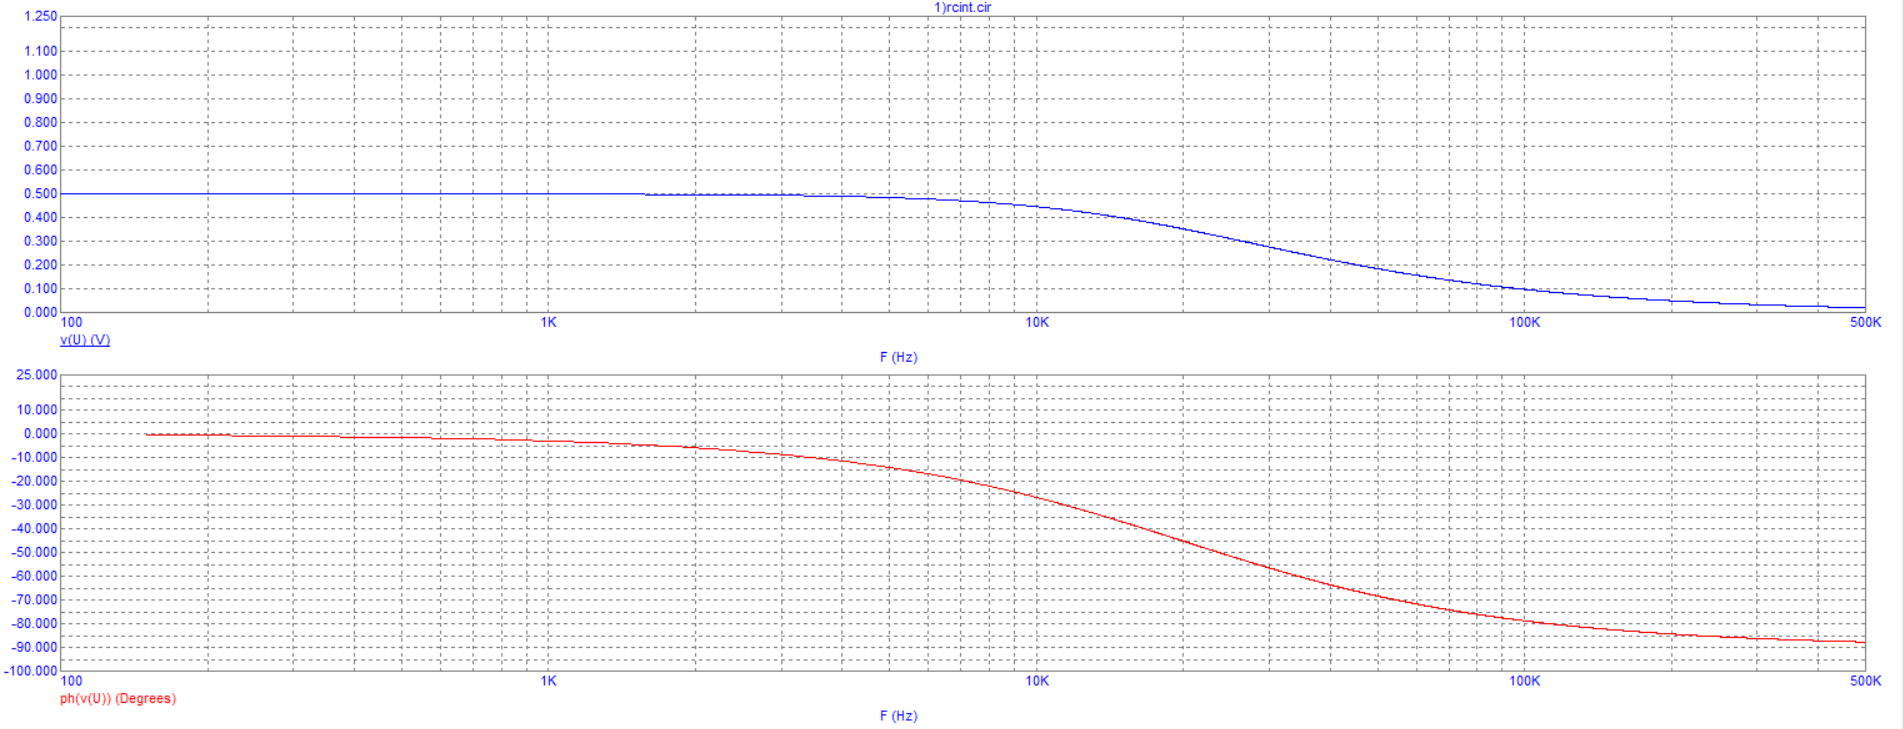
\includegraphics[width=1\textwidth]{1_5.png}
	\label{fig:boiler}
\end{figure}

\newpage1

а для R = 10 МОм: $f_0(10 \text{МОм}) = 10 \text{ кГц}$

\begin{figure}[!h]
	\centering
	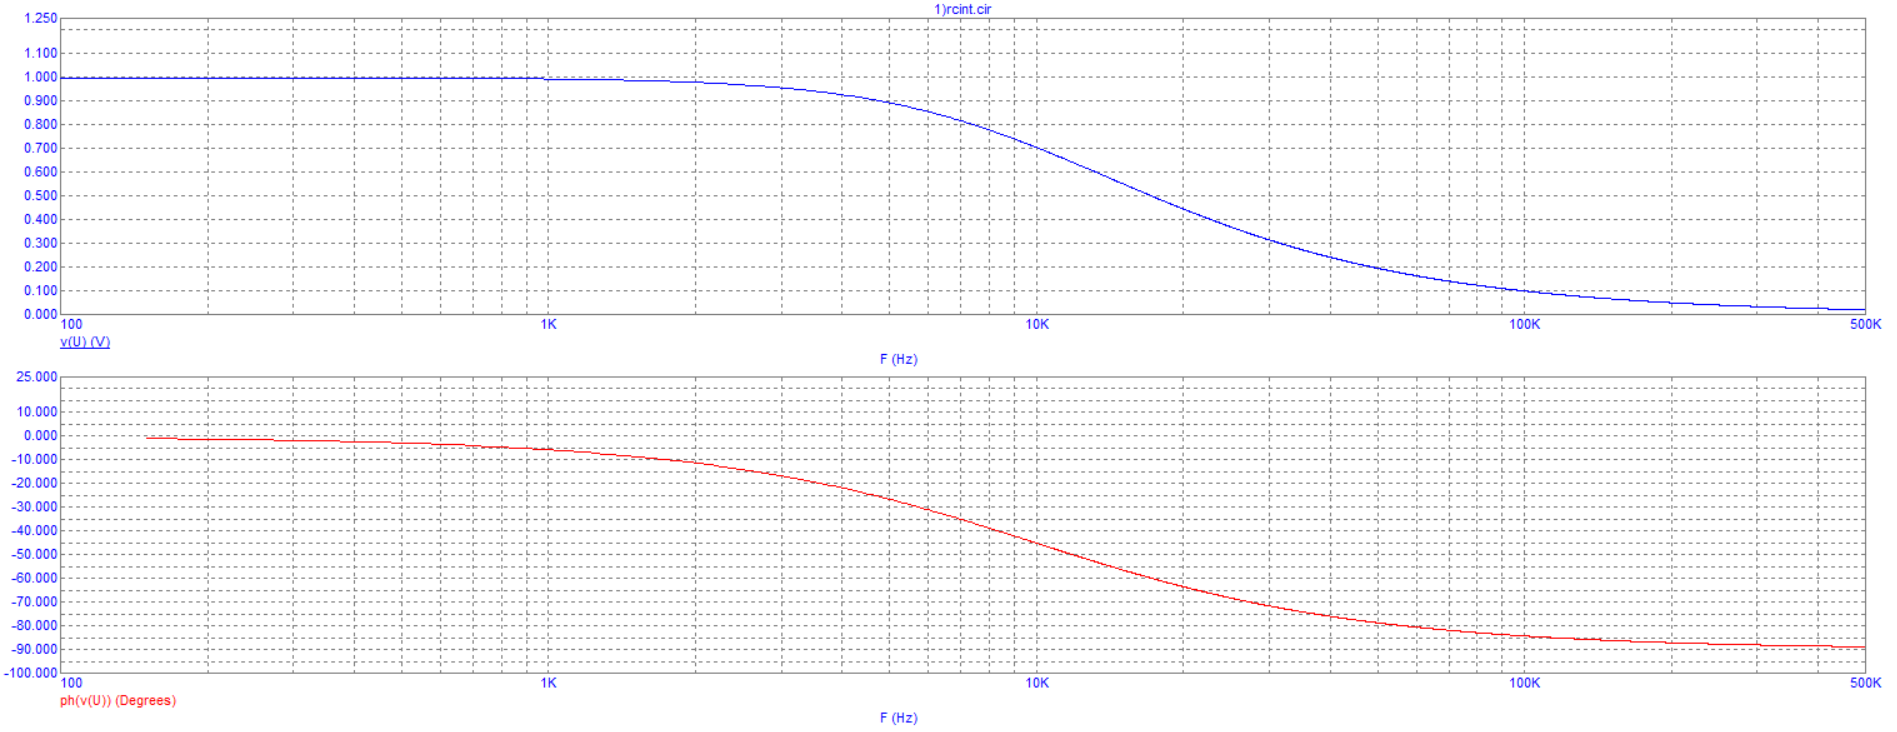
\includegraphics[width=1\textwidth]{1_4.png}
	\label{fig:boiler}
\end{figure}

Для режима переходной характеристики легко рассчитать, что

\begin{figure}[!h]
	\centering
	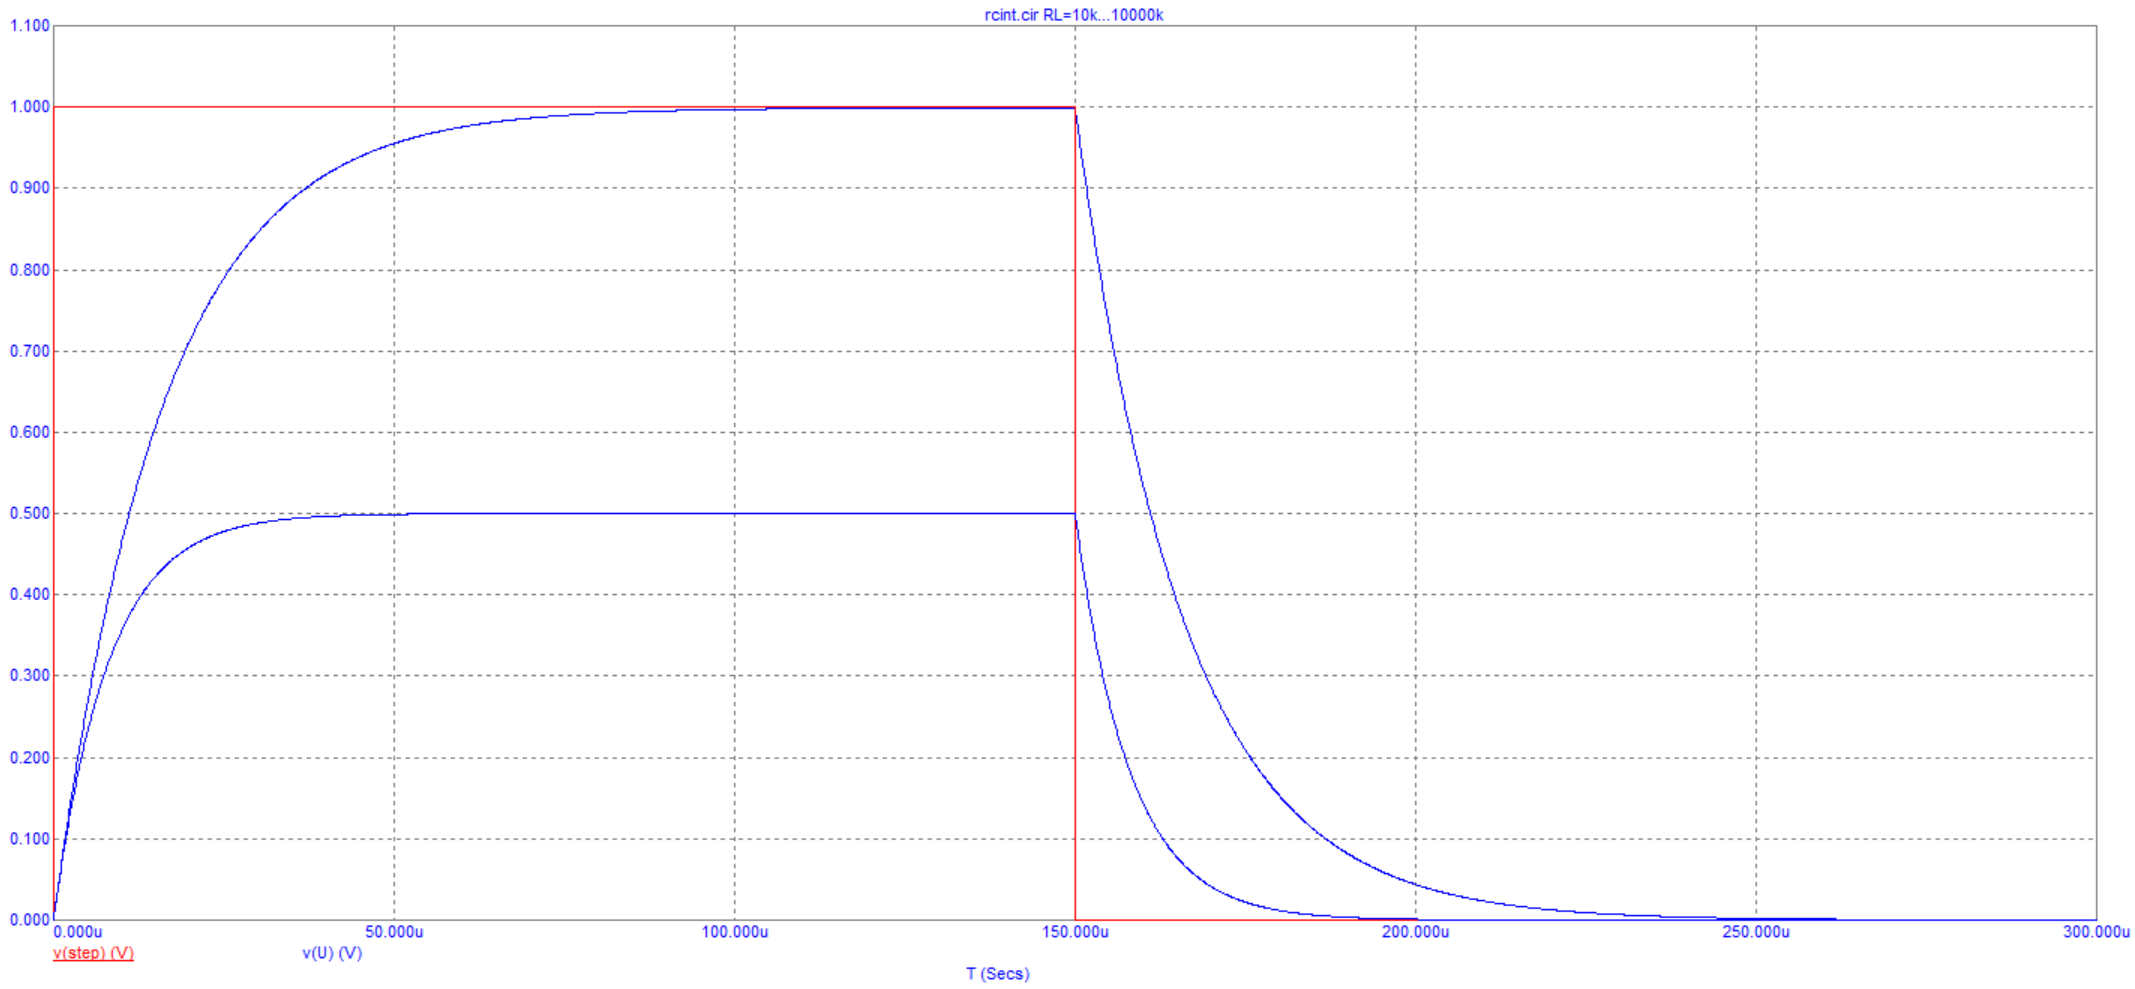
\includegraphics[width=1\textwidth]{1_7.png}
	\label{fig:boiler}
\end{figure}

\begin{equation}
	R_L = 10 \text{ кОм: } \tau = 8.014 \text{ мкс}
\end{equation}

\begin{equation}
	R_L = 10 \text{ МОм: } \tau = 16.027 \text{ мкс}
\end{equation}

что почти идеально совпадает с теоретическими значениями

\begin{equation}
	R_L = 10 \text{ кОм: } \tau = 8 \text{ мкс}
\end{equation}

\begin{equation}
	R_L = 10 \text{ МОм: } \tau = 15.984 \text{ мкс}
\end{equation}

6) Рассмотрим модель rcdiff.cir.

\begin{figure}[!h]
	\centering
	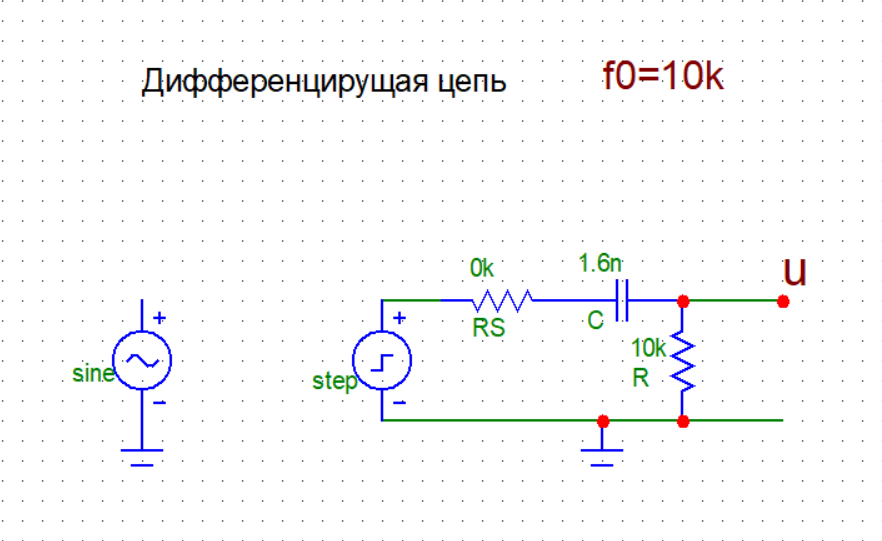
\includegraphics[width=1\textwidth]{1_8.png}
	\label{fig:boiler}
\end{figure}

\newpage

 Её фазо-частотная характеристика

\begin{figure}[!h]
	\centering
	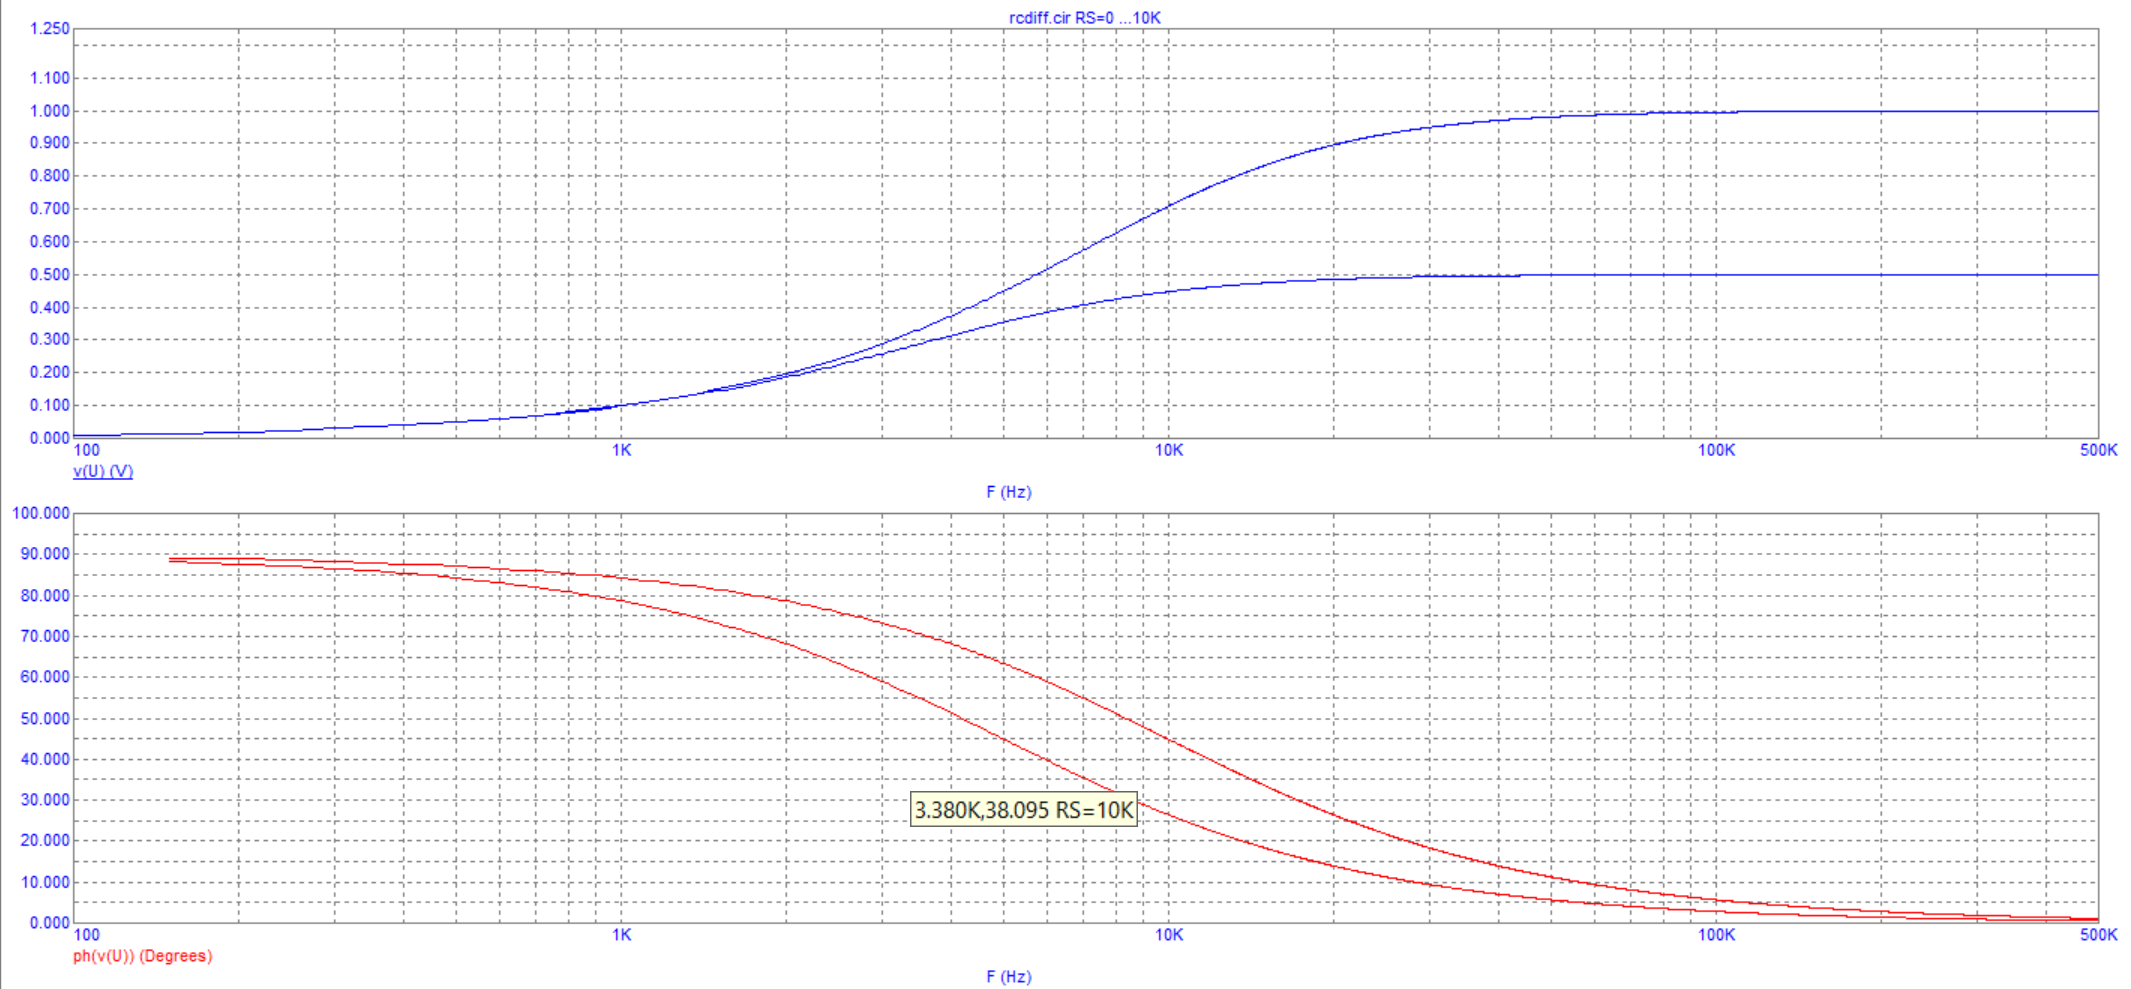
\includegraphics[width=1\textwidth]{1_9.png}
	\label{fig:boiler}
\end{figure}

Передаточная функция при этом

\begin{equation}
	H(p) = \frac{K_0 p \tau}{1 = p \tau} \text{ ; } K_0 = \frac{R}{R+R_S} \text{ ; } \tau = (R + R_S) C
\end{equation}

Верхняя частота же

\begin{equation}
	R_S = 0; f_0 = \text{10 кГц}
\end{equation}

\begin{equation}
	R_S = 10 \text{ кОм}, f_0 = 5\text{ кГц}
\end{equation}

Переходная характеристика схемы

\begin{figure}[!h]
	\centering
	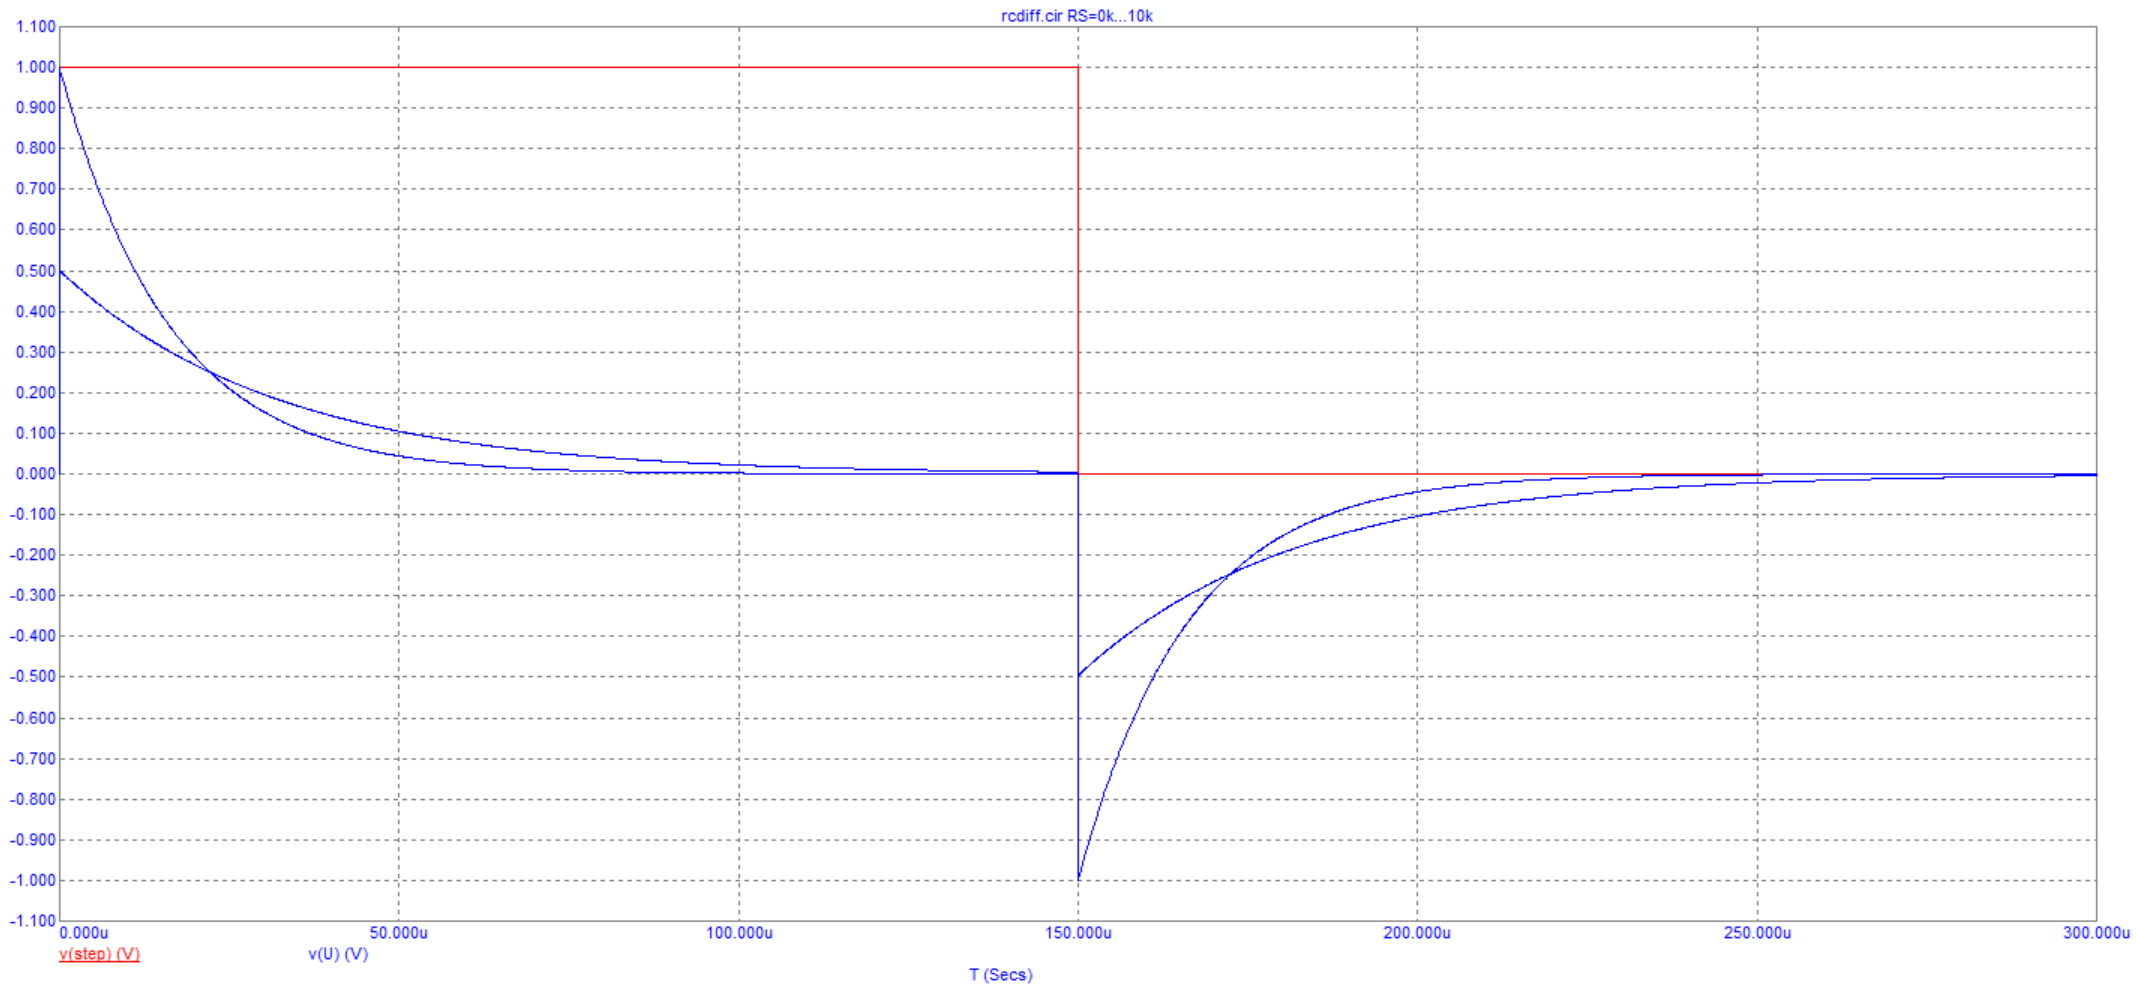
\includegraphics[width=1\textwidth]{1_10.png}
	\label{fig:boiler}
\end{figure}

Постоянная времени

\begin{equation}
	R_S = 0; \tau = 16.071\text{ мкс}
\end{equation}

\begin{equation}
	R_S = 0 \text{ кОм}, \tau = 32.141\text{ мкс}
\end{equation}

7) Откроем модель rcpower.cir. 

\begin{figure}[!h]
	\centering
	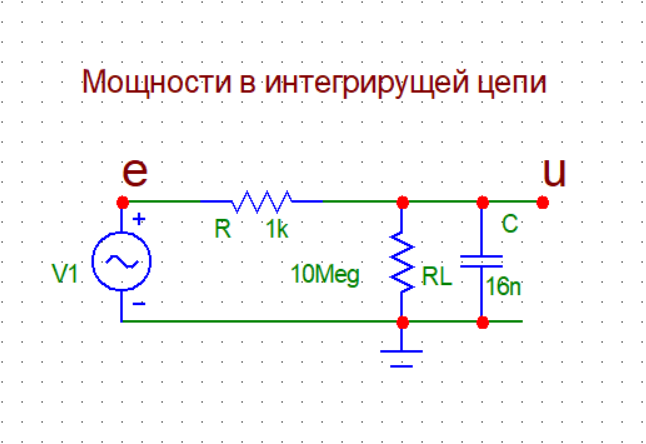
\includegraphics[width=1\textwidth]{1_11.png}
	\label{fig:boiler}
\end{figure}

\newpage

Изучим графики частотной зависимости потребляемых интегрирующей цепью активных и реактивных мощностей и графики мощностей на её комопонентах

\begin{figure}[!h]
	\centering
	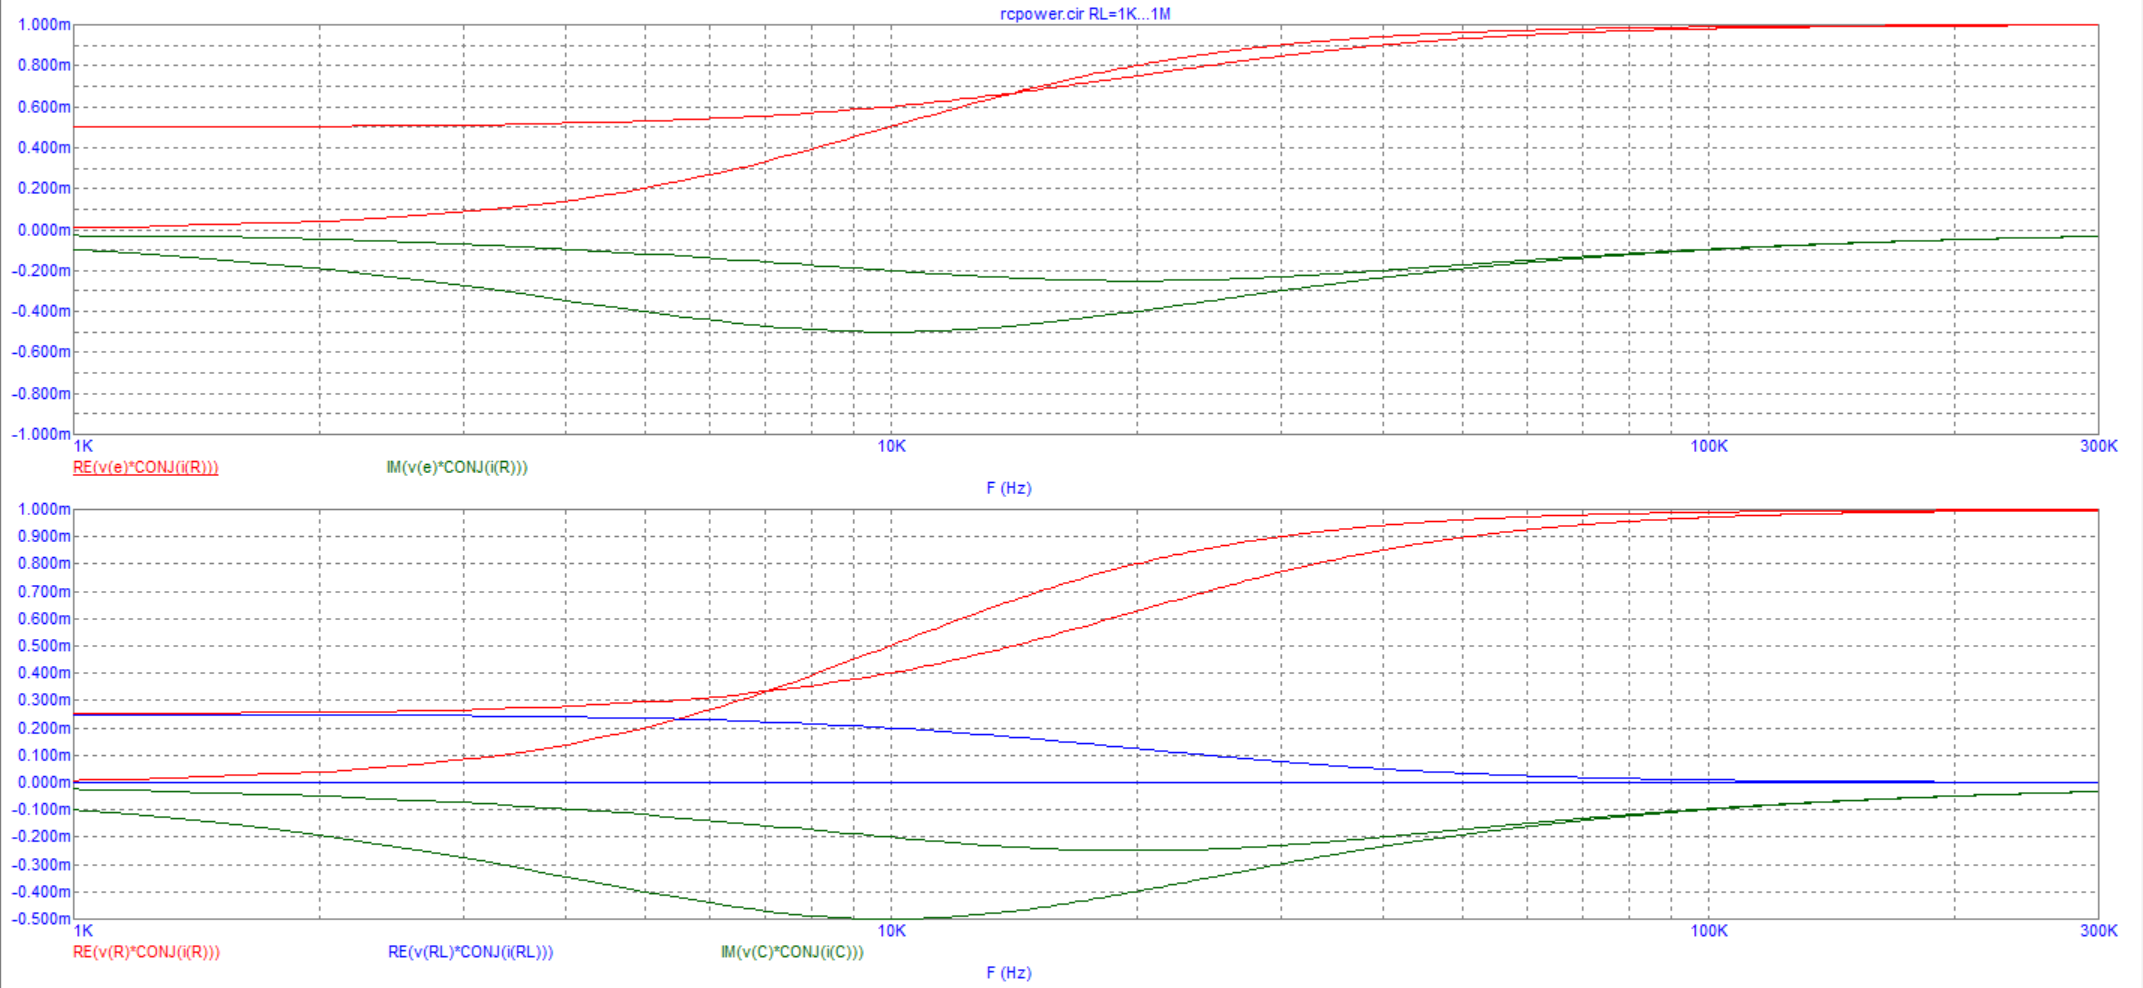
\includegraphics[width=1\textwidth]{1_12.png}
	\label{fig:boiler}
\end{figure}

Видно, что у реактивной компоненты потребление становится максимальным при частоте f$_0$ = 10 кГц, и стремится к нулю при частоте f = 0 и f = $\inf$.

При f = f$_0$
выполняется закон сложения мощностей, то есть модули действительной и комплексной частей мощности одинаковы.

Подключая и отключая резитор $R_L$ варьированием $[1k, 1Meg \vert 1Meg] (1Meg = \infty)$, изучим его влияние на распределение мощностей в схеме при $f = f_0$.

При уменьшении значения сопротивления резистора $R_L$, его мощность возрастает до 0.2 мВт вместо нуля, мощность на резисторе $R$ падает до 0.4 мВт с 0.5 мВт, а реактивная мощность конденсатора падает до 0.2 с 0.5 мВт.


\subsubsection{Вывод}

В практической части задания теоретические расчеты довольно хорошо согласуются с практикой, граф Боде же качественно демонстрирует состоятельность выбранной модели. У соответствующего подбора сопротивлений и емкостей есть существенный спад кожффициента передачи при низких частотах, что связано непосредственно с неидеальностью генератора, но в данном случае эта область достаточно далека от исследуемого диапазона, чтобы её можно было не учитывать.

\subsection{RC-звенья второго порядка}

\subsubsection{Теория}

Передаточная функция произвольной двухполюсной системы приводится к виду $H(s)=\frac{a s^2+b s+c}{s^2+2 \xi s+1}$ и представляется взвешенной суммой передаточных функций полиномиальных звеньев трех типов - фильтра верхних частот (ФВЧ), полосового фильтра (ПФ) и фильтра нижних частот (ФНЧ):
$$
H(s)=\frac{a s^2+b s+c}{s^2+2 \xi s+1}=a \frac{s^2}{s^2+2 \xi s+1}+b \frac{s}{s^2+2 \xi s+1}+c \frac{1}{s^2+2 \xi s+1} .
$$
Эти звенья различаются положением нулей - у ФВЧ имеется нуль кратности два в нуле, у ФНЧ - нуль кратности два в бесконечности. Полосовой фильтр (ПФ) занимает промежуточное положение: один нуль в бесконечности, второй - в нуле.

При малых добротностях $Q=\frac{1}{2 \xi}<\frac{1}{2}$ такие звенья удается реализовать каскадным соединением звеньев первого порядка, как показано на рис. 13. Выбор пар одинаковых резисторов и конденсаторов дает звенья с $2 \xi=3, Q=\frac{1}{2 \xi}=\frac{1}{3}$. Полюсы их передаточных функций вещественны и находятся в точках $s_{ \pm}=-\mu_{ \pm}$, $\mu_{ \pm}=\frac{3 \pm \sqrt{5}}{2}\left(\mu_{+} \simeq 2.62, \mu_{-} \simeq 0.38\right)$.

Комплексный коэффициент передачи полосового звена с $H(s)=\frac{s}{s^2+3 s+1}, s=\frac{j \omega}{\omega_0}$ приводится к виду
$$
K(j \omega)=\frac{1}{3+\left(s+\frac{1}{s}\right)}=\frac{1}{3} \frac{1}{(1+j a(\omega))} ; \quad a(\omega)=\frac{1}{3}\left(\frac{\omega}{\omega_0}-\frac{\omega_0}{\omega}\right) .
$$
Коэффициент передачи ФВЧ отличается множителем $s=\frac{j \omega}{\omega_0}$ в числителе, а коэффициент передачи ФНЧ - таким же множителем в знаменателе.

\begin{figure}[!h]
	\centering
	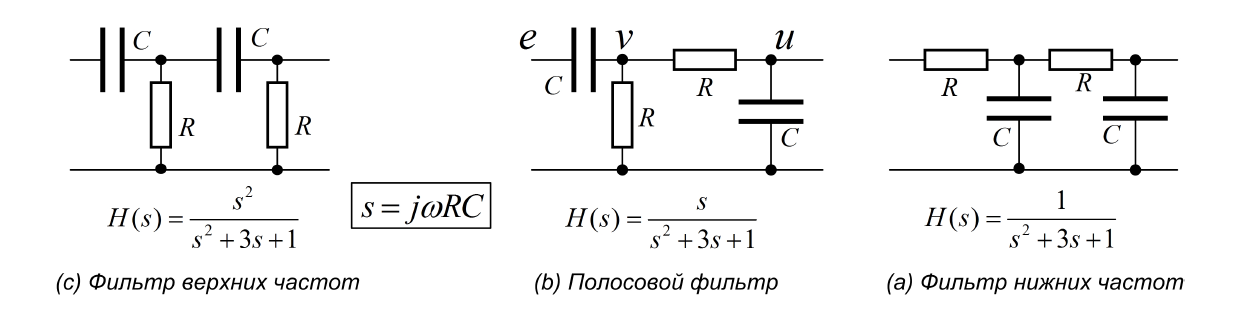
\includegraphics[width=1\textwidth]{2_1.png}
	\label{fig:boiler}
\end{figure}

Граф Боде фильтра нижних частот показан на рис. На
логарифмической оси относительной частоты $lg \frac{f}{f_0}$ показаны два полюса $lg \mu_{\pm} = lg \left( \frac{3 \pm \sqrt{5}}{2} \right)$ Ломаная линия графа приходит из минус бесконечности (от нулевой частоты) с уровнем 0 dB. Излом в полюсе $\mu_{\_}$ добавляет спад со скоростью 20 dB на
декаду. Второй излом в полюсе $\mu_{+}$ поднимает скорость спада до
40 dB на декаду. В нуле, на частоте $f_0$, достигается затухание $\frac{1}{3} = -9.5$ dB.

\begin{figure}[!h]
	\centering
	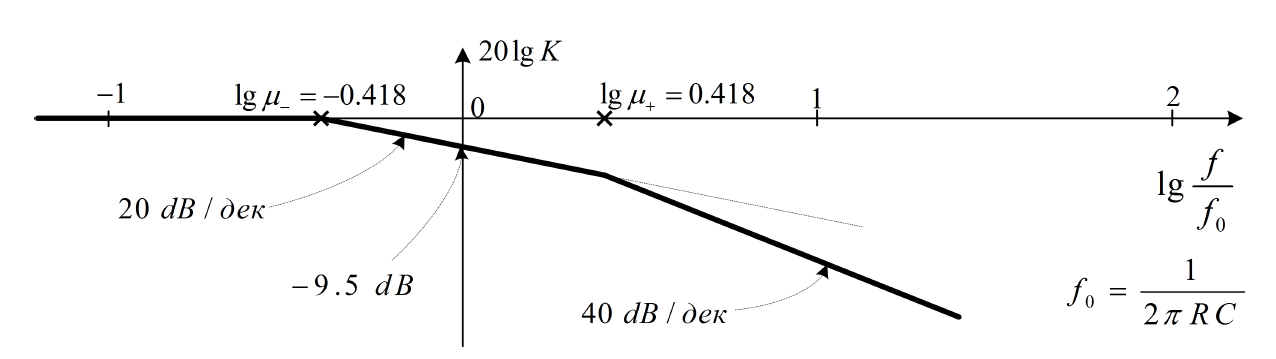
\includegraphics[width=1\textwidth]{2_2.png}
	\label{fig:boiler}
\end{figure}

Переходные характеристики звеньев являются линейны-
ми комбинациями быстро и медленно затухающих экспонент $e^{-(\mu_+)\frac{t}{\tau}}$, $e^{-(\mu_{\_})\frac{t}{\tau}}$, $\tau = R C$. Характерные времена спада этих экспонент различаются в $\frac{\mu_{+}}{\mu_{\_}} = 7$ раз.

\subsubsection{Выполнение}

Откроем файл rc2pole.cir

\begin{figure}[!h]
	\centering
	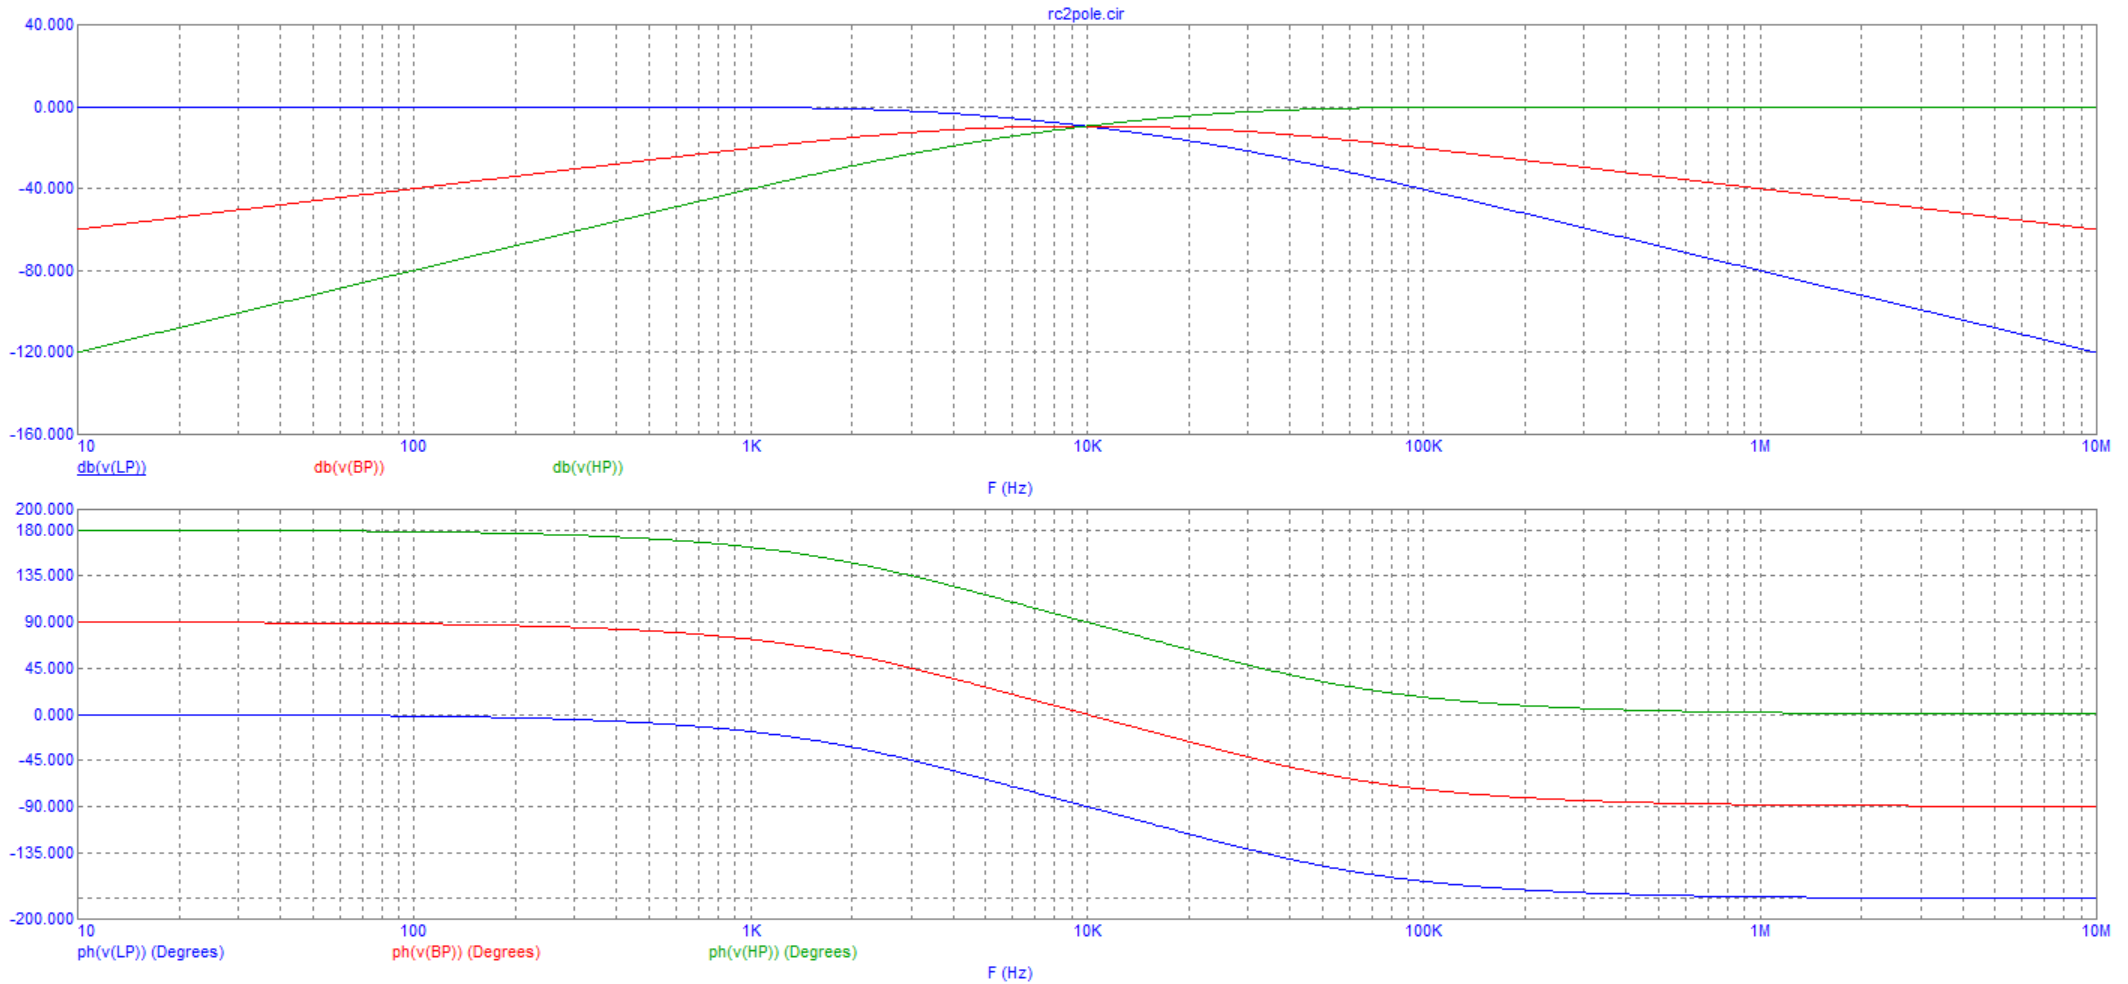
\includegraphics[width=1\textwidth]{2_4.png}
	\label{fig:boiler}
\end{figure}

По графикам определим затухание на частоте $f_0 \simeq 10 $ кГц, оно равно -9.55 dB и скорость его нарастания в полосах задержания -40.4 + 9.55 = -30.85 dB/декаду. По графикам  ФЧХ измерим значения фазовых сдвигов  ФВЧ, ПФ и ФНЧ на частотах 0, $f_0$, $\infty$.

\begin{center}
\begin{tabular}{|c|c|c|c|}
\hline 
 & ФВЧ & ПФ & ФНЧ \\ 
\hline 
0 & 180 & 90 & 0 \\ 
\hline 
$f_0$ & 90 & 0 & -90 \\ 
\hline 
$\infty$ & 0 & -90 & -180 \\ 
\hline 
\end{tabular} 
\end{center}

Двухсторонняя полоса $\triangle f$ пропускания ПФ $\approx$ 29.76 кГц, что в три раза больше $f_0$. Это совпадает с теорией.

2) Откроем графики переходных характеристик

\begin{figure}[!h]
	\centering
	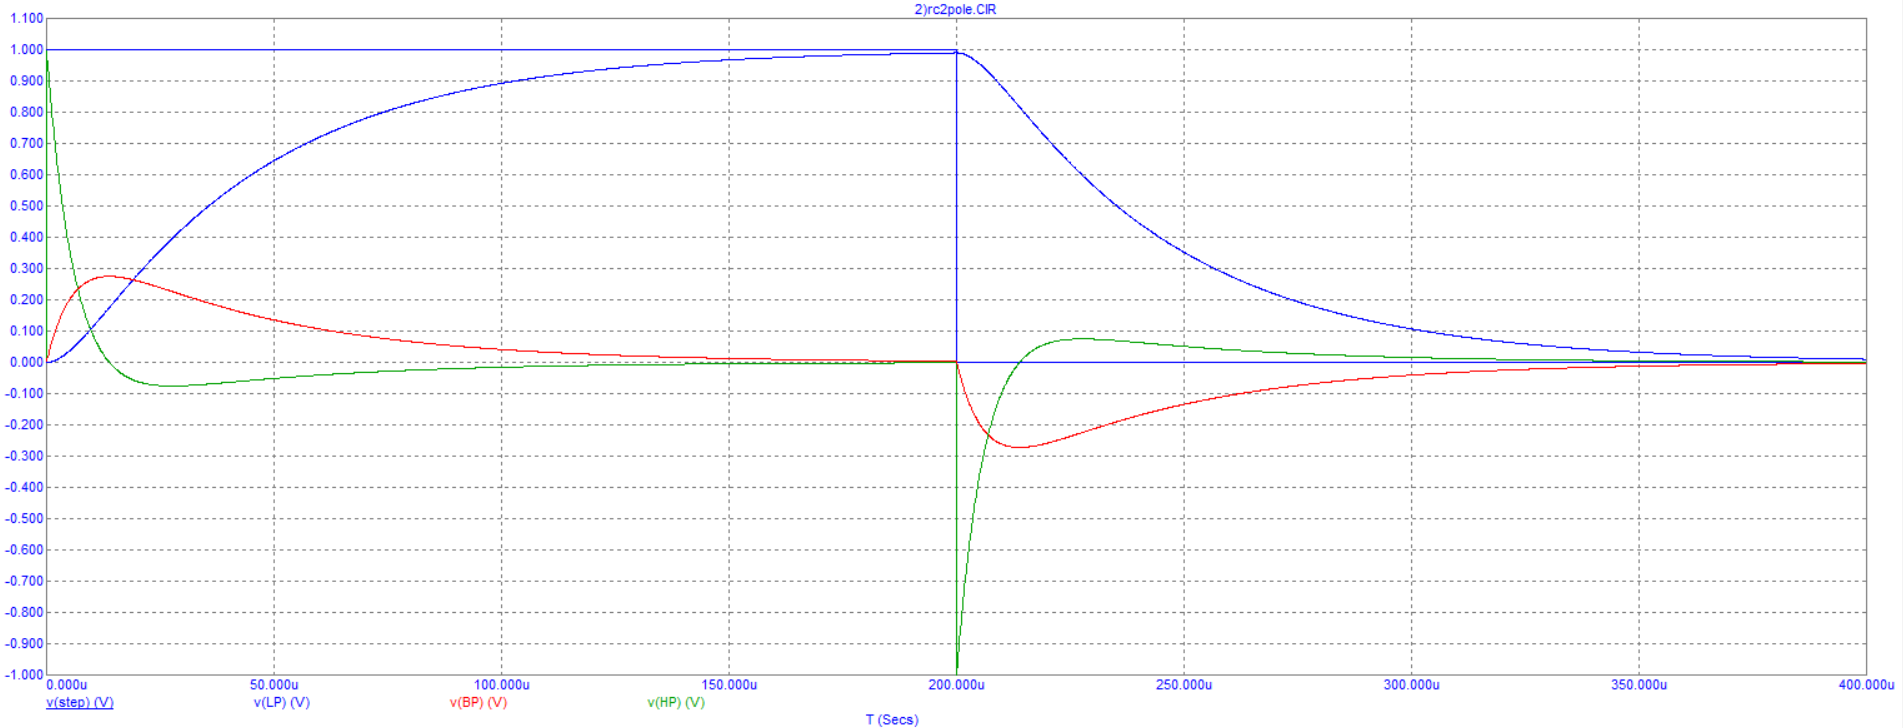
\includegraphics[width=1\textwidth]{2_3.png}
	\label{fig:boiler}
\end{figure}

Оценим время спада $\tau_-$ первого выброса переходной характеристик ФВЧ до уровня $1/e \simeq 0,37$:

\[\tau_-= 4.97 \: \text{мкс}\]

Оценим время нарастания $t_+$ фронта переходной характеристики ФНЧ до уровня $1 - 1/e \simeq 0.63$:

\[\tau_+ = 48.5 \: \text{мкс}\]

Найдем их отношение:

\[\frac{\tau_+}{\tau_-} = 9.76\]


\subsubsection{Вывод}

Теория хорошо совпадает с моделированием

\subsection{Мостовые схемы}

\subsubsection{Теория}

Полезными специфическими свойствами отличаются схемные
решения с топологией мостов, рис. 16a. Мостовую конфигурацию образуют четыре соединенные прямоугольником импеданса. Входной сигнал e прикладывается к одной диагонали моста, а выходной u снимается с другой.

Выходной сигнал моста является разностным (дифференциальным). Он получается вычитанием выходов левого ($Z_1$/$Z_2$) и правого ($Z_3$/$Z_4$) делителей напряжения. Передаточная функция моста это разность передаточных функций двух делителей. Вычитание дает эффект взаимной компенсации сигналов, поступающих на выход моста по одному и другому пути. Это приводит к передаточным функциям с нетипичным расположением нулей - мостовыми схемами реализуются неминимально фазовые системы с нулями в правой полуплоскости и системы с комплексно-сопряженными парами нулей.

\begin{figure}[!h]
	\centering
	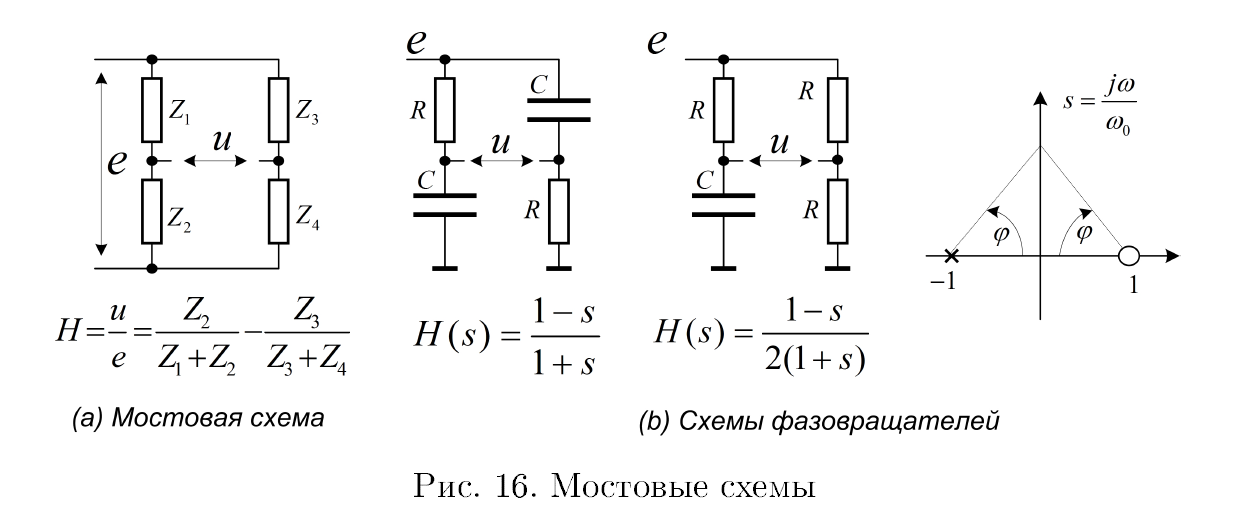
\includegraphics[width=1\textwidth]{3_3.png}
	\label{fig:boiler}
\end{figure}

Простые примеры неминимально фазовых цепей показаны на рис. 16b. Их передаточные функции имеют полюс в левой полуплоскости при s = -1 и симметрично расположенный нуль в правой полуплоскости при s = 1. Модуль коэффициента передачи этих цепей постоянен: расстояния от точки $s = \frac{j \omega}{\omega_0}$ до полюса и нуля всегда одинаковы. Фазовая же характеристика отличается аномально большим набегом фазы вклад полюса, изменяющийся от нуля до $-\pi/2$, суммируется с таким же
вкладом нуля. Результатом становится фазовая характеристика $\phi(\omega) = -2 arctg\left( \frac{\omega}{\omega_0} \right)$ с вариацией от нуля до $-\pi$.

Схема двойного T-моста на рис. 17 топологически представляет собой фазовращатель на рис. 16b, в выходную диагональ которого включена дополнительная RC-цепочка. Приведенная на рисунке передаточная функция моста замечательна наличием пары комплексно сопряженных нулей в точках $\pm j$ на мнимой оси s-плоскости. Ее полюсы вещественны и расположены в точках $s = -\mu{\pm}$, $\mu_{\pm} = 2 \pm \sqrt{3}$ ($\mu_{+} \simeq 3.73$, $\mu_{\_} = 0.27$, $\mu_{+} / \mu_{\_} \simeq 14$).
Нули на мнимой оси дают эффект обращения в нуль модуля коэффициента передачи при s = j, то есть при $\omega = \omega_0 = \frac{1}{R C}$.

Двойной T-мост это режекторный фильтр, который пол-
ностью подавляет частоту $\omega_0$. Его комплексный коэффициент
передачи приводится к виду

\begin{equation}
	K(j \omega) = \frac{1}{1 + \frac{4}{j a(\omega)}} \text{ ; } a(\omega) = \left( \frac{\omega}{\omega_0} - \frac{\omega_0}{\omega} \right)
\end{equation}

Границы полосы режекции по уровню $\frac{1}{\sqrt{2}} = -3$ dB достигаются при |a| = 4. Это дает $\Delta \omega = 4 \omega_0$

\begin{figure}[!h]
	\centering
	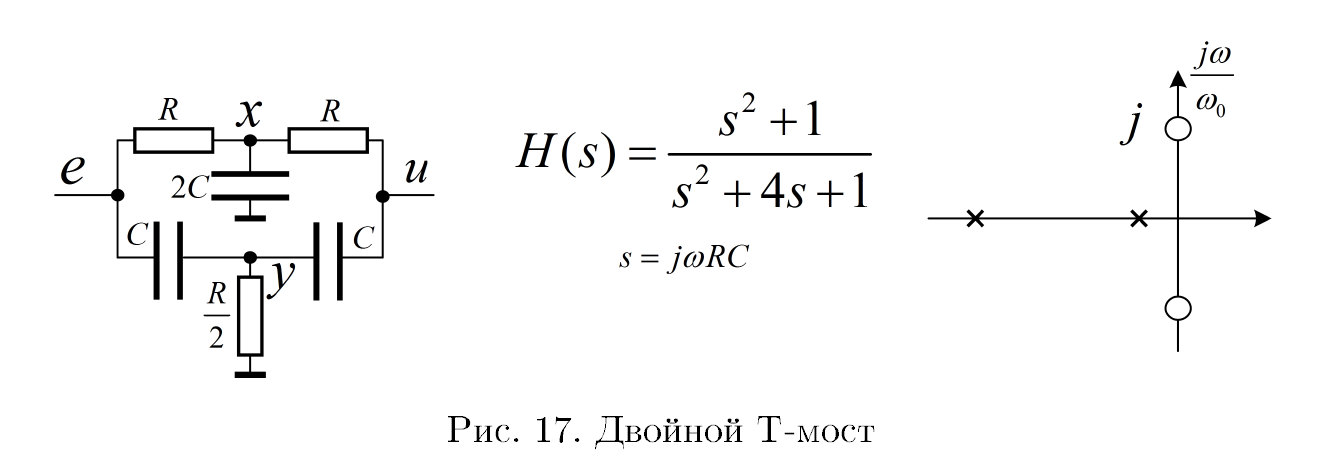
\includegraphics[width=1\textwidth]{3_4.png}
	\label{fig:boiler}
\end{figure}

\subsubsection{Выполнение}

1) Откроем модель фазовращателя(phshift.cir)

\begin{figure}[!h]
	\centering
	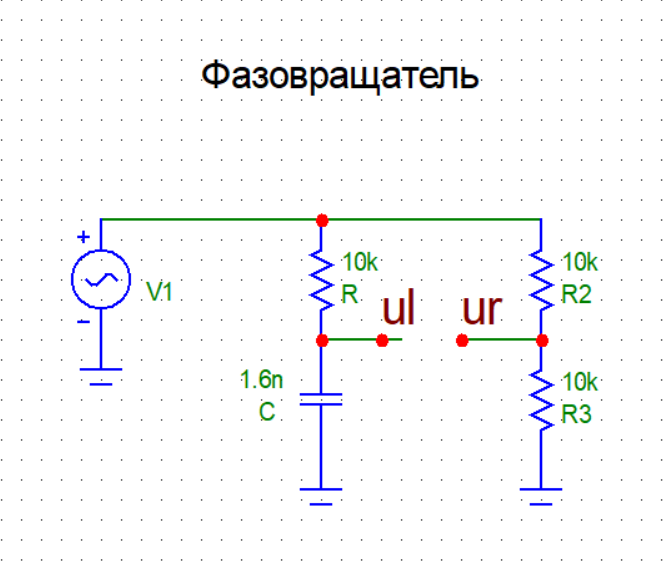
\includegraphics[width=1\textwidth]{3_1.png}
	\label{fig:boiler}
\end{figure}

Наибольший диапазон перестройки реализуется на частоте $f = 20  \: \textit{кГц}$. Границы этого диапазона $[-154.9; -33.4]$.

\begin{figure}[!h]
	\centering
	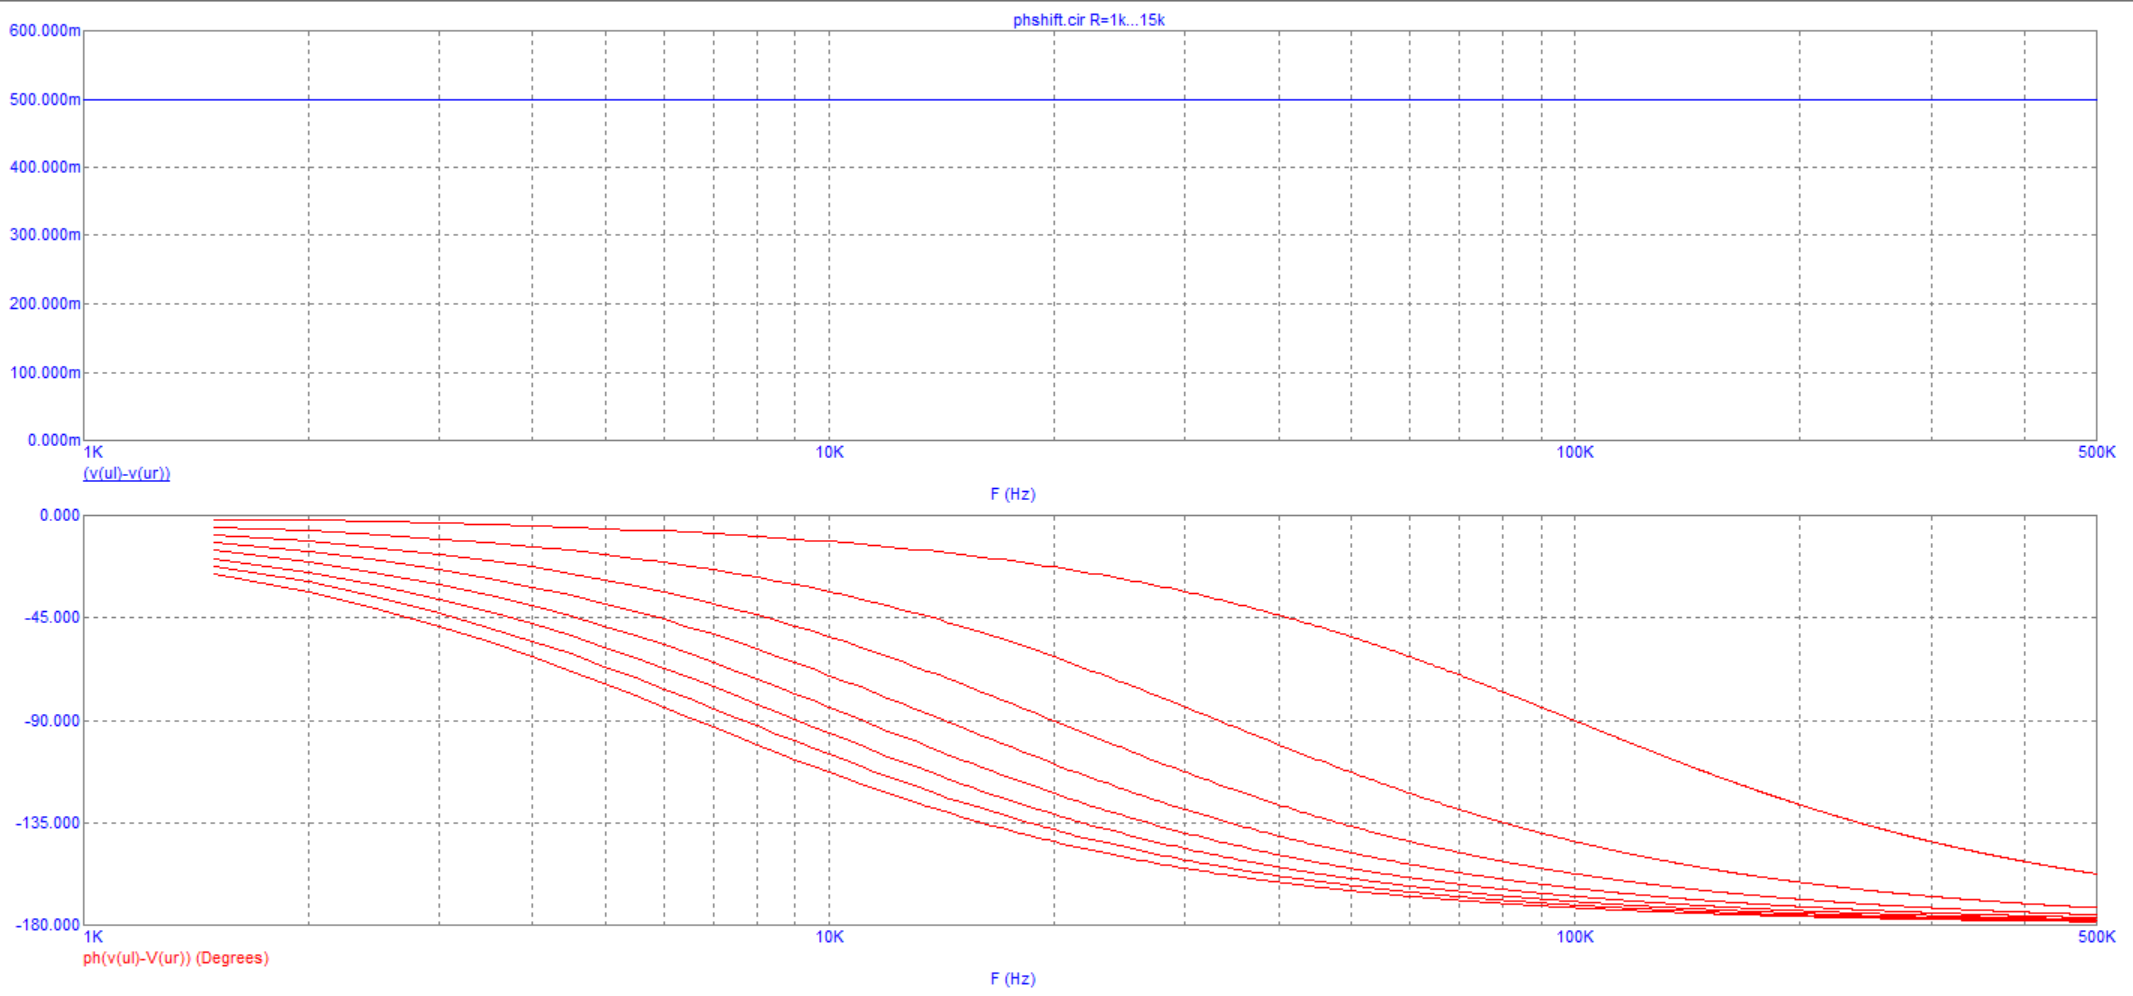
\includegraphics[width=1\textwidth]{3_2.png}
	\label{fig:boiler}
\end{figure}

2) Откроем модель двойного Т-моста 2tbridge.cir.

\begin{figure}[!h]
	\centering
	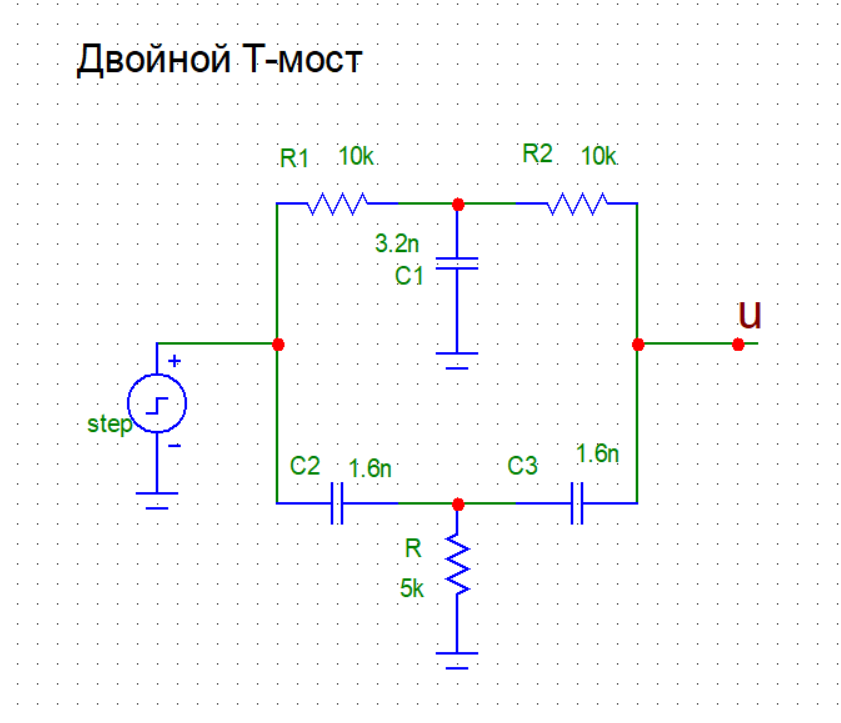
\includegraphics[width=1\textwidth]{3_5.png}
	\label{fig:boiler}
\end{figure}

Измерим полосу режекции $\triangle f = 38.98 \: \text{кГц}$. $f_0 = 10 \: \text{кГц}$, следовательно выполняется $\triangle f = 4 f_0$.

\begin{figure}[!h]
	\centering
	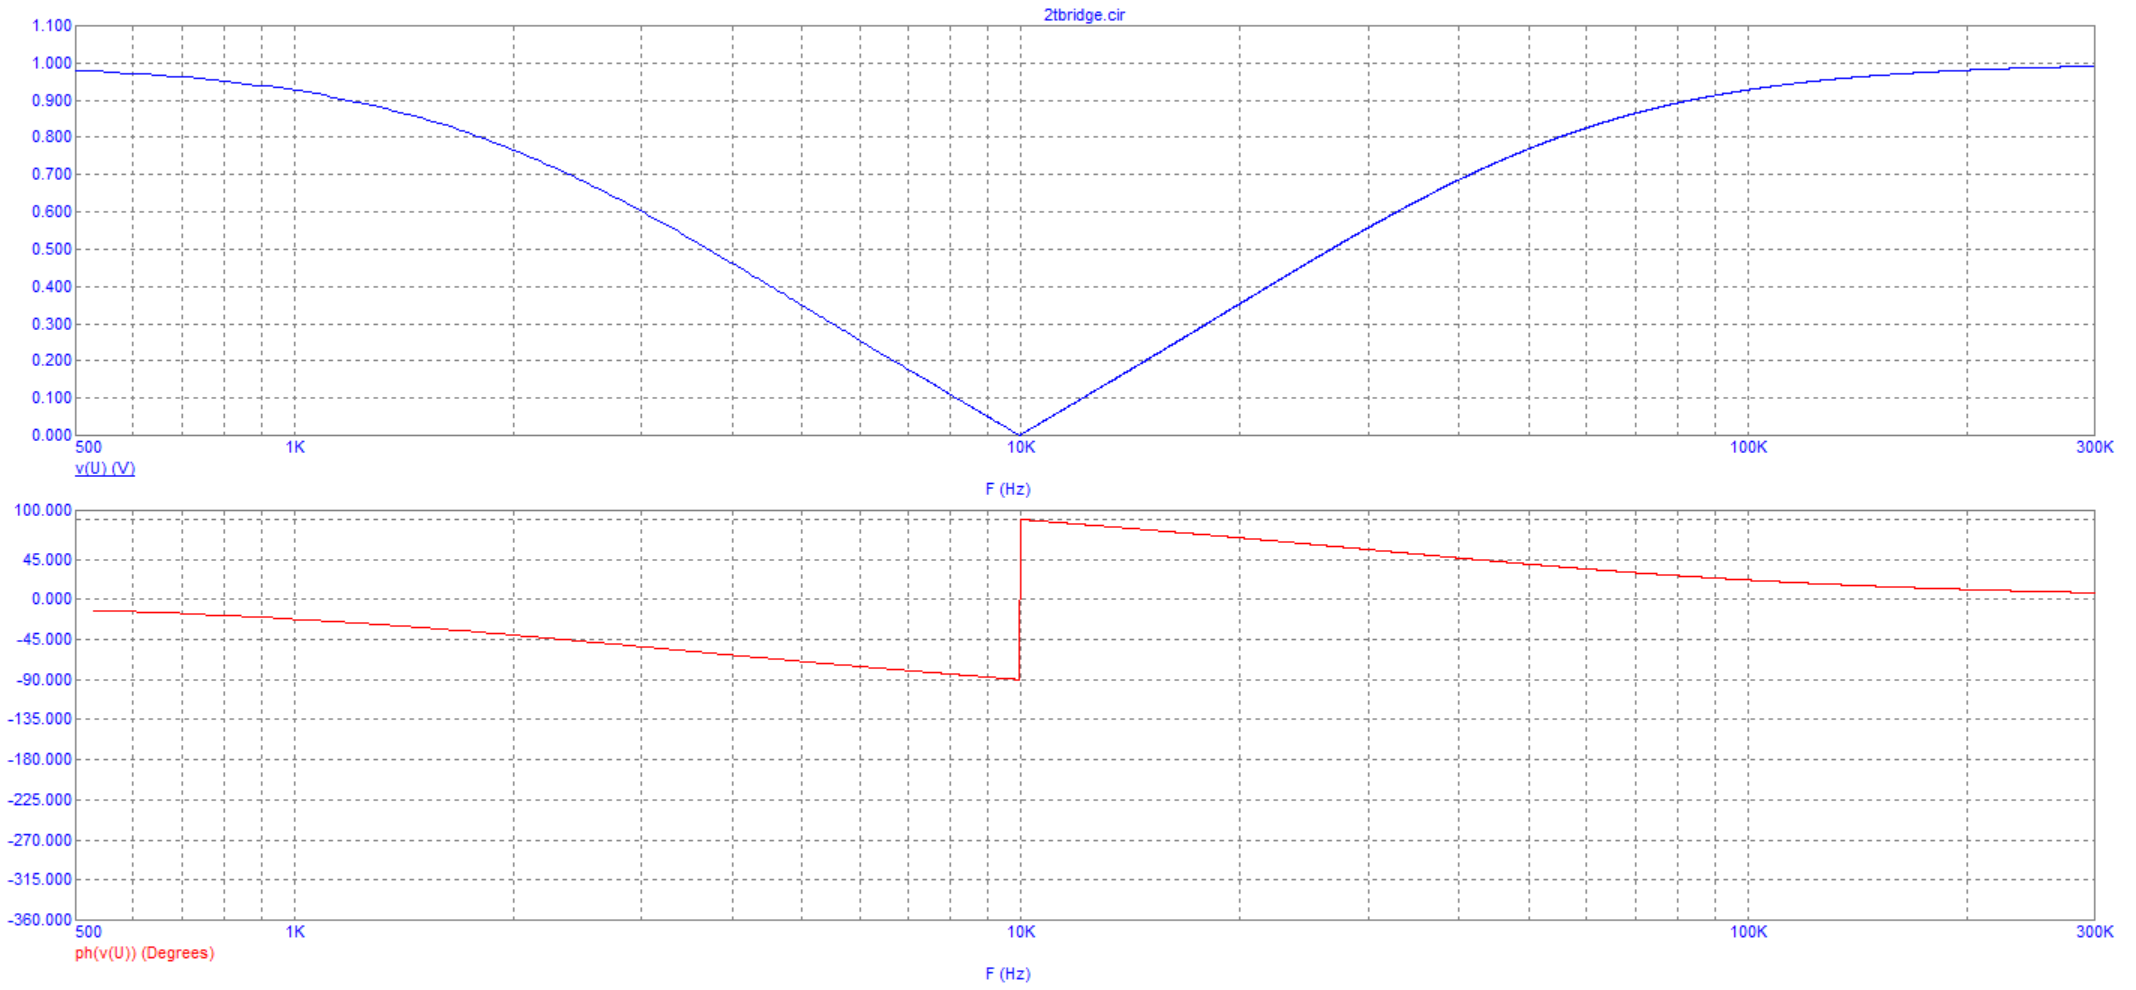
\includegraphics[width=1\textwidth]{3_6.png}
	\label{fig:boiler}
\end{figure}

При варьировании сопротивления, при его росте, $f_0$ падает. При $R = 5 \: \textit{кОм}$ наблюдается скачок на ФЧХ.

\begin{figure}[!h]
	\centering
	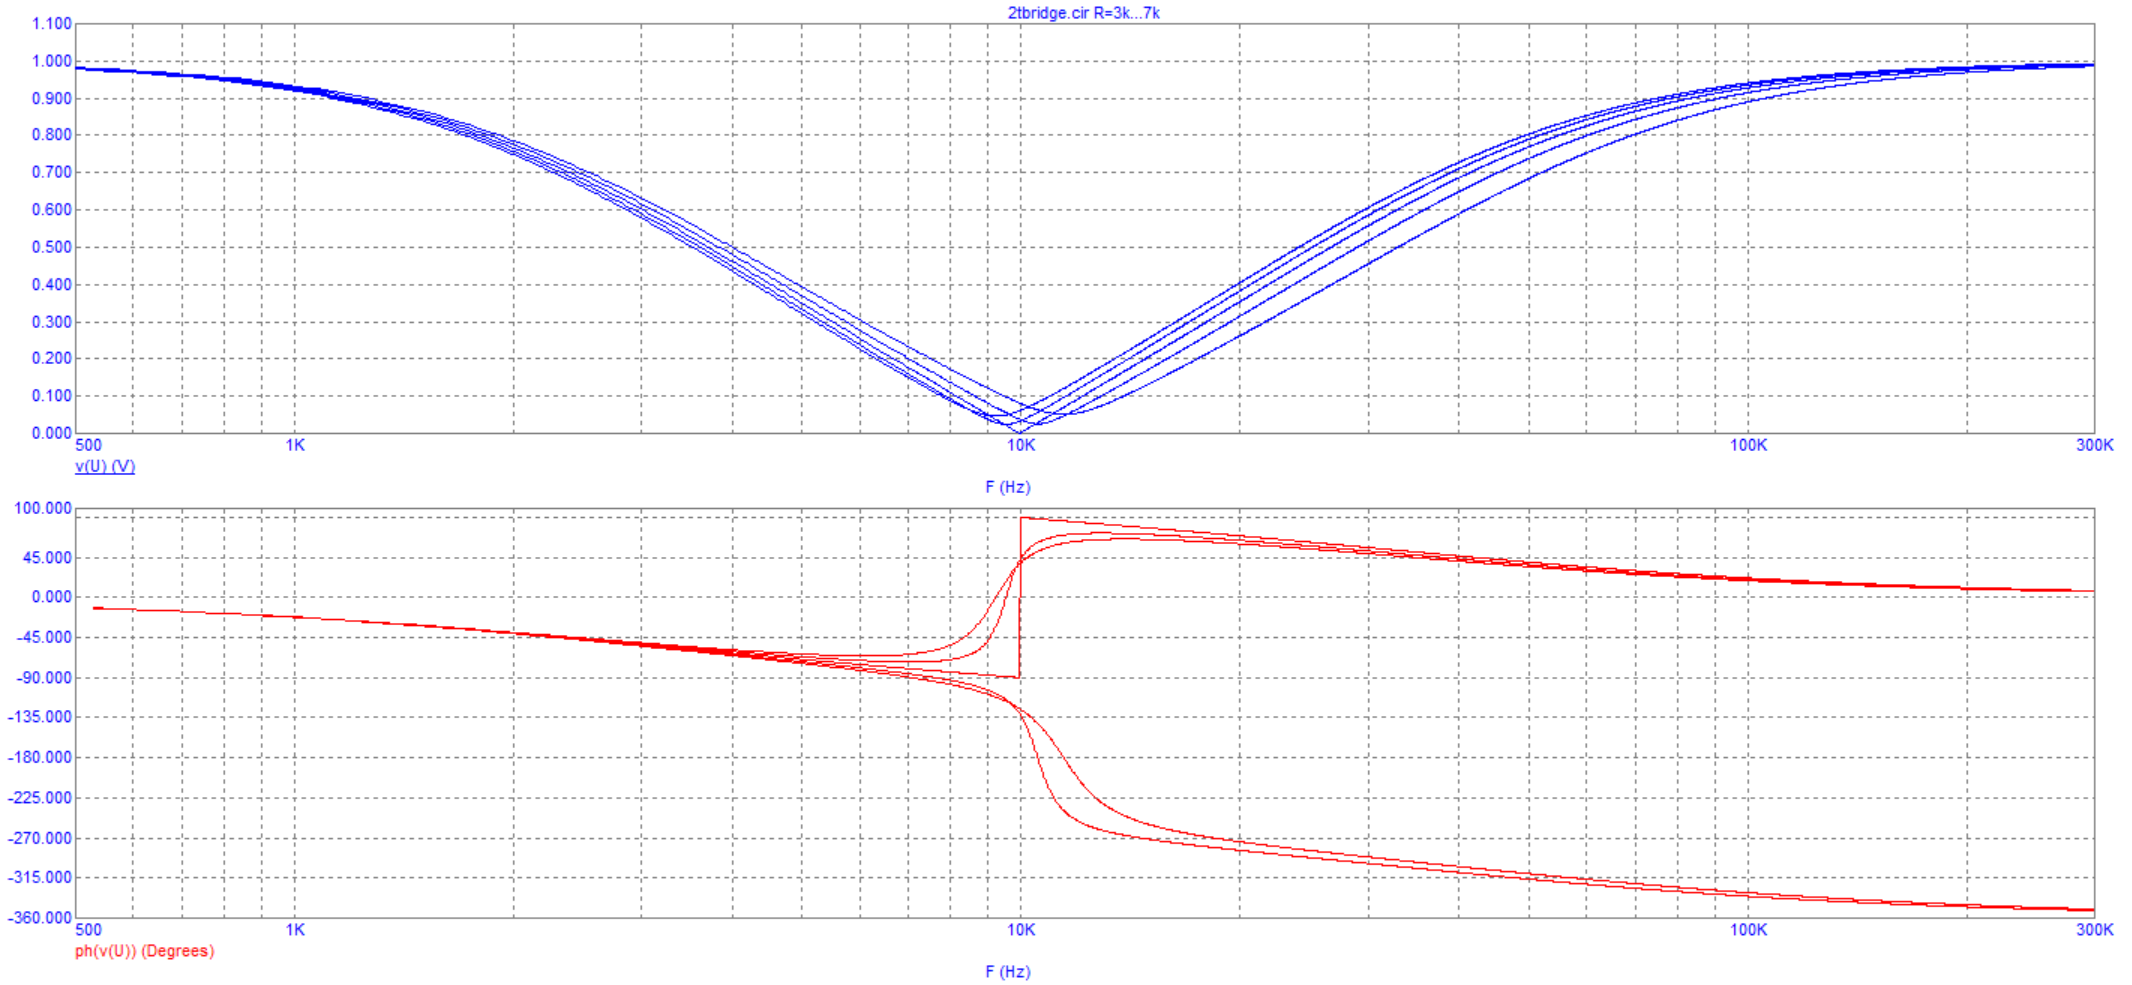
\includegraphics[width=1\textwidth]{3_7.png}
	\label{fig:boiler}
\end{figure}

\newpage

\begin{figure}[!h]
	\centering
	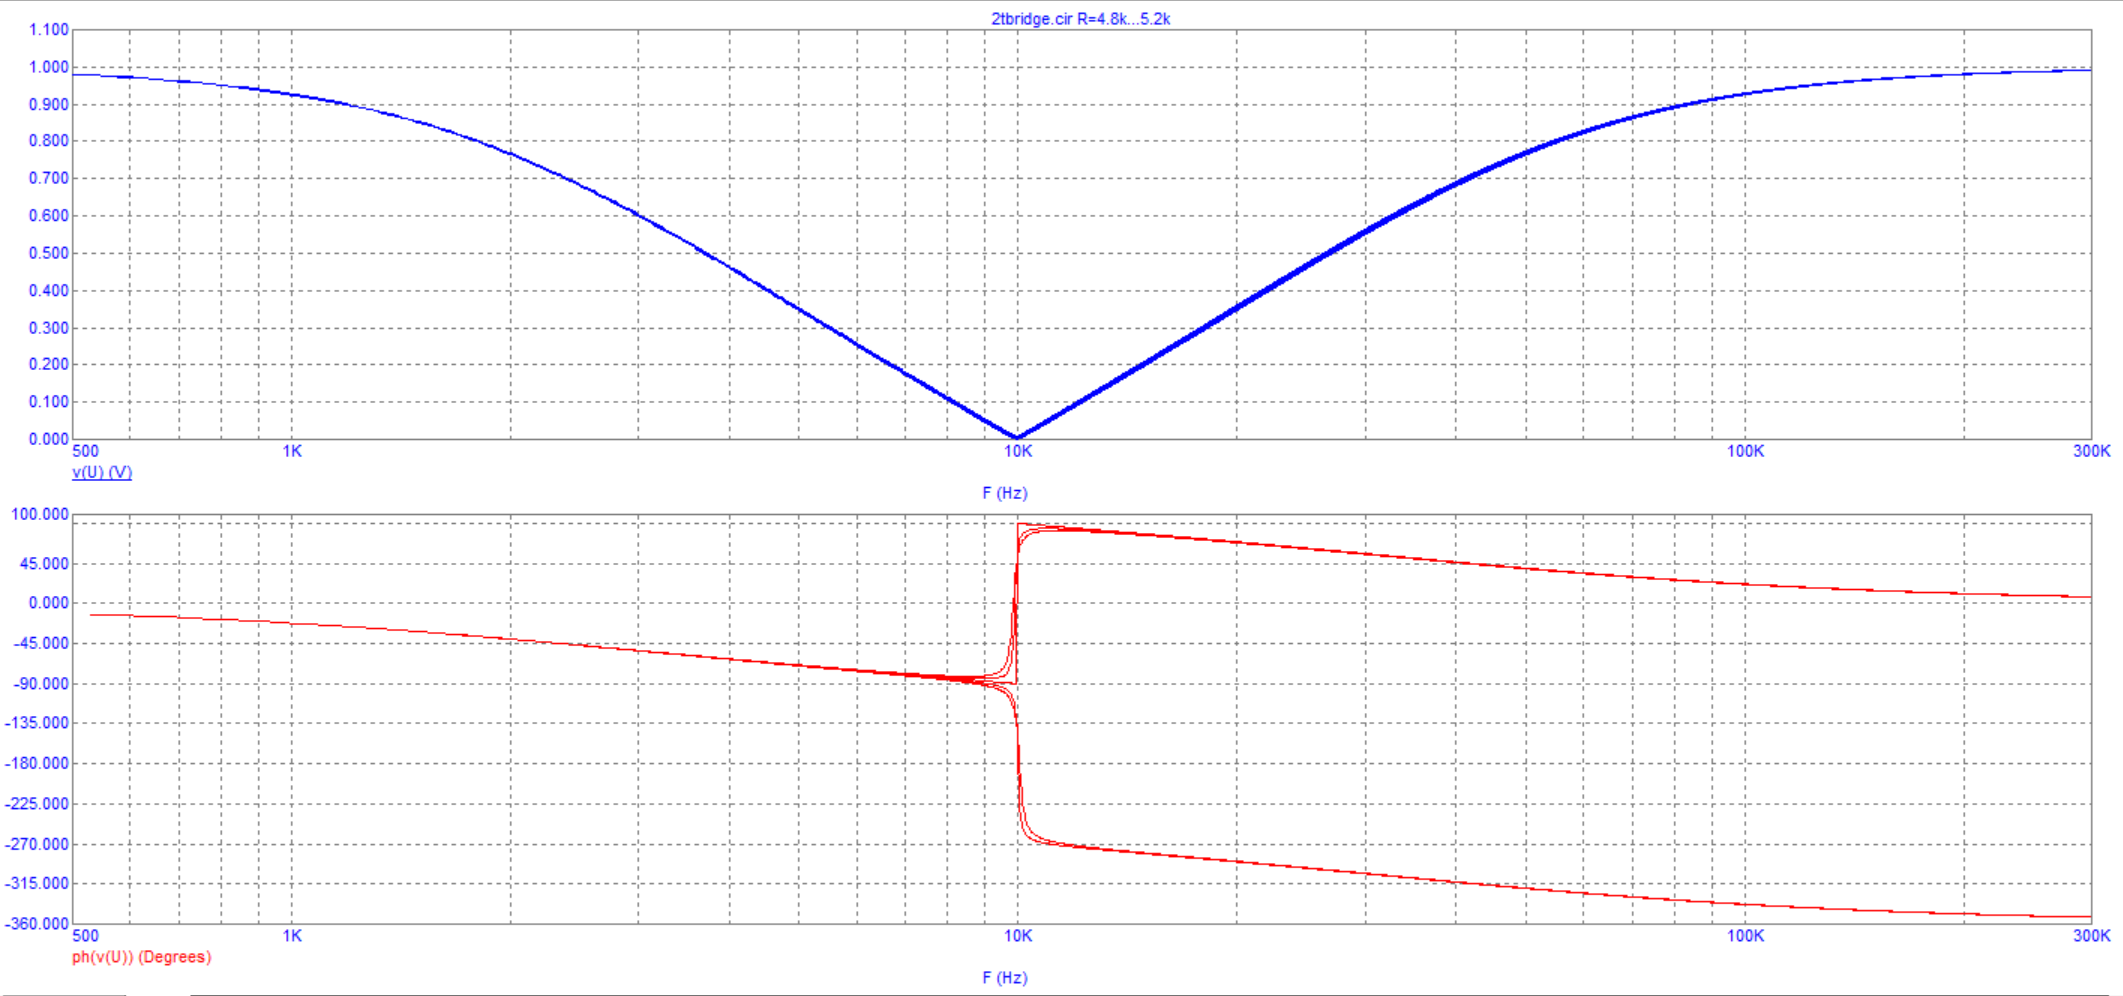
\includegraphics[width=1\textwidth]{3_8.png}
	\label{fig:boiler}
\end{figure}

3) Подключив ко фходу источник прямоугольного импульса, проанализиурем переходную характеристику. $\tau_+ = 4 \: \text{мкс}$, $\tau_- = 58 \: \text{мкс}$. Это сходится с теоретическими значениями($\tau = \frac{1}{2 \pi f_0 \mu_{\pm}}$, $\mu_{\pm} = 2 \pm \sqrt{3}$)

Варьирование сохраняет площадь под графиком функции, тем самым усредняя её.

\begin{figure}[!h]
	\centering
	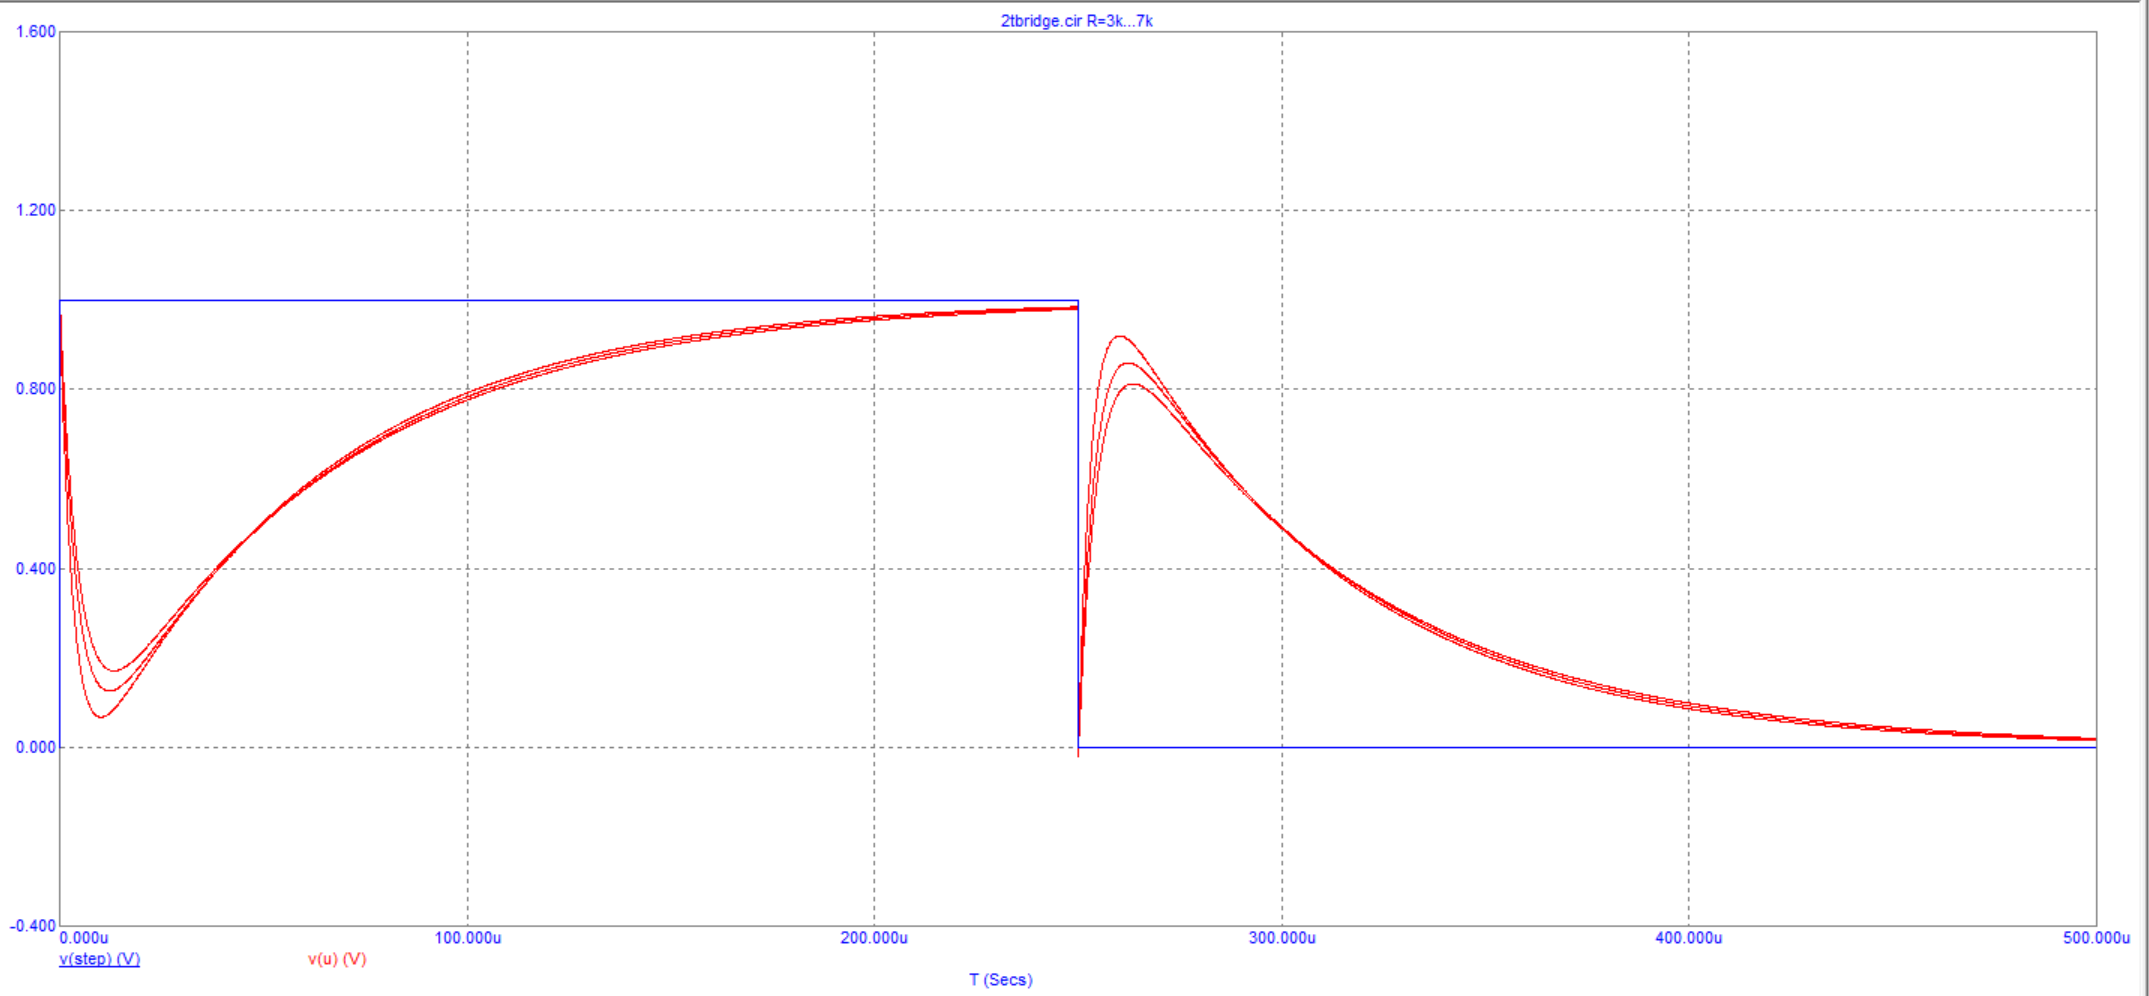
\includegraphics[width=1\textwidth]{3_9.png}
	\label{fig:boiler}
\end{figure}

\newpage

4) Откроем модель 2tdelay.cir

\begin{figure}[!h]
	\centering
	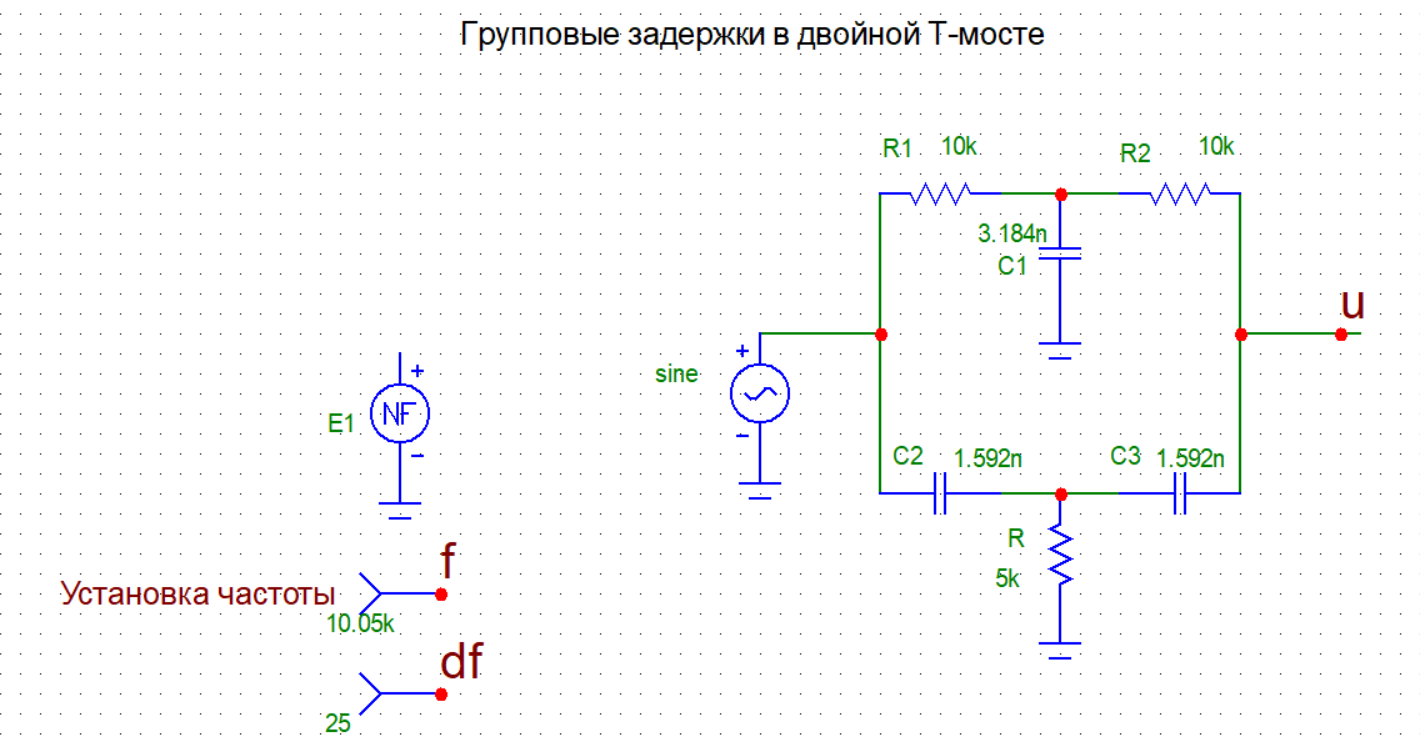
\includegraphics[width=1\textwidth]{3_10.png}
	\label{fig:boiler}
\end{figure}

Оценим $Q = f_0/\Delta f$.

\begin{figure}[!h]
	\centering
	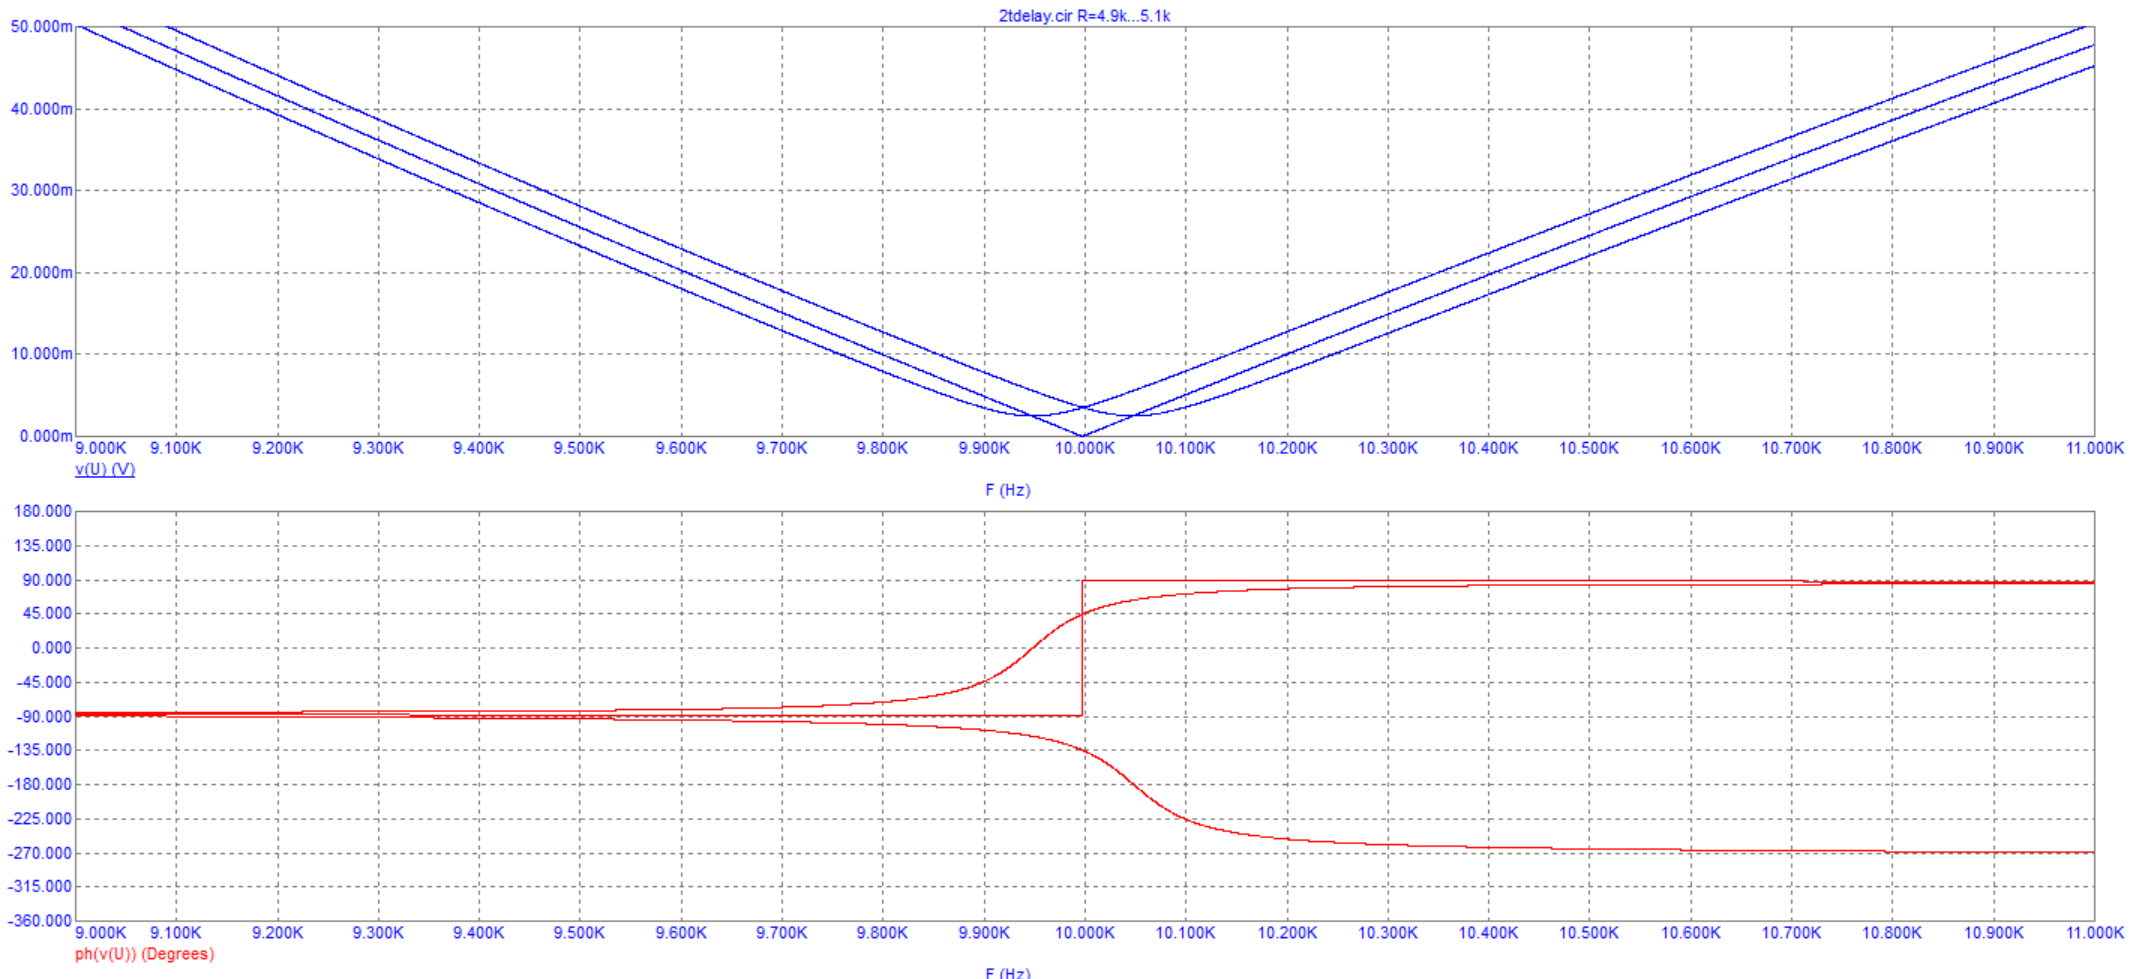
\includegraphics[width=1\textwidth]{3_11.png}
	\label{fig:boiler}
\end{figure}

\begin{center}
\begin{tabular}{|c|c|c|c|}
\hline 
$R, \: \textit{кОм}$ & 4.9 & 5 & 5.1 \\ 
\hline 
$f_0, \: \textit{кГц}$ & 10.05 & 10 & 9.95 \\ 
\hline 
$\triangle f, \: \textit{кГц}$ & 0.05 & $ 2.5 \cdot 10^{-4}$ & 0.05 \\ 
\hline 
$Q$ & 100.5 & 40000 & 99.5 \\ 
\hline 
\end{tabular}
\end{center}

\begin{figure}[!h]
	\centering
	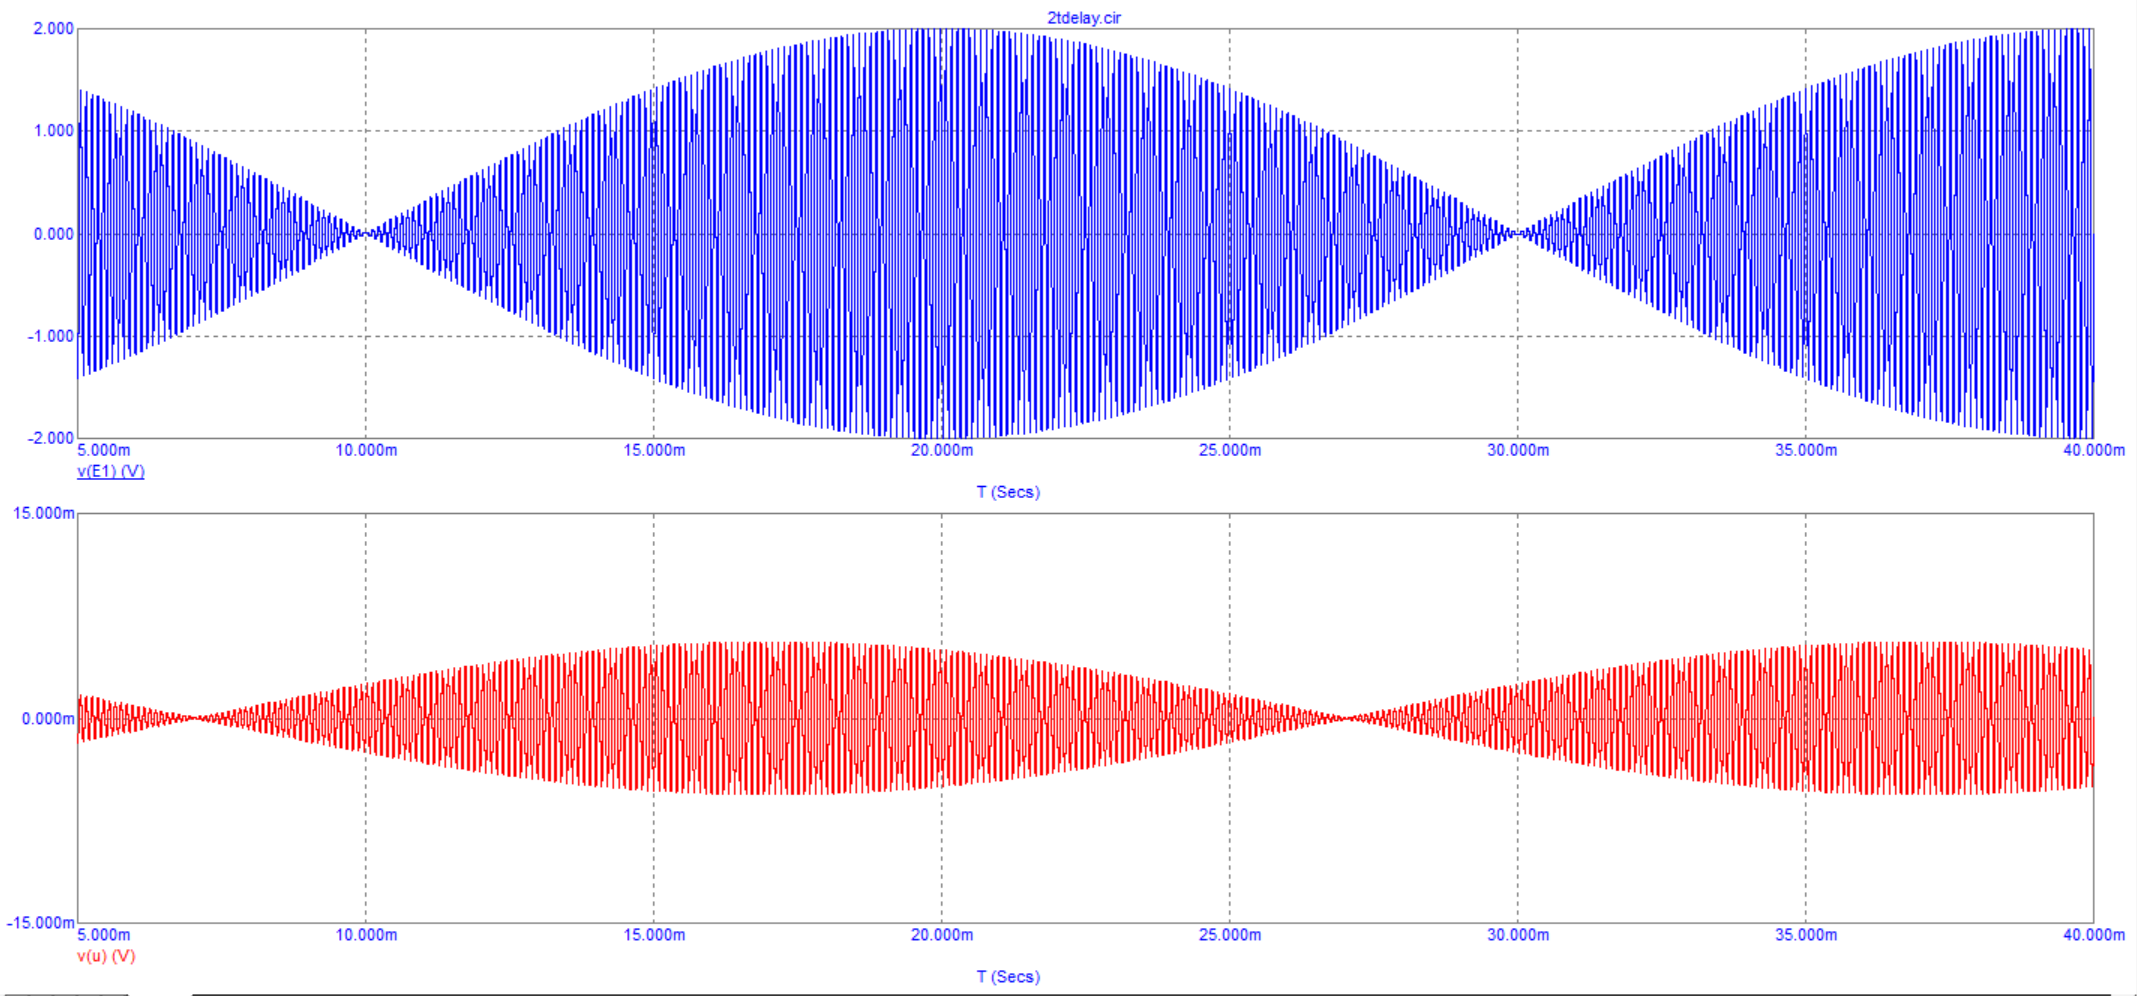
\includegraphics[width=1\textwidth]{3_12.png}
	\label{fig:boiler}
\end{figure}

В режиме $\text{Transient}$ измерим групповые задержки $\tau_g$

\[\tau_g = 2.94 \: \text{мс}\]

для обоих R и f.

\subsubsection{Вывод}

Теория хорошо совпадает с практикой.

\subsection{Последовательный резонанс}

\subsubsection{Теория}

\begin{figure}[!h]
	\centering
	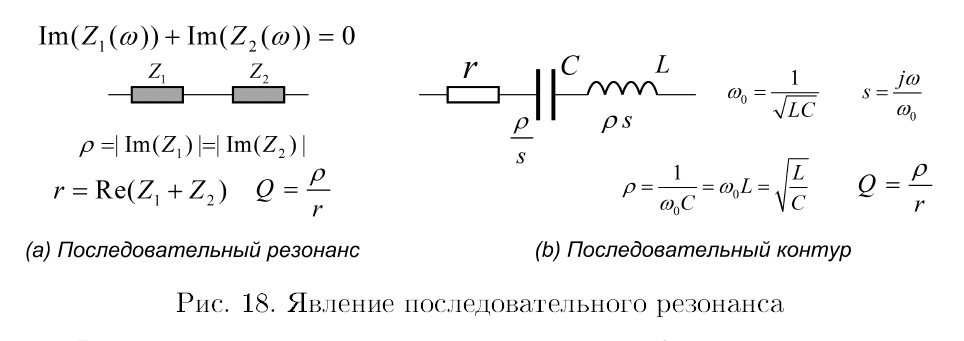
\includegraphics[width=1\textwidth]{4_1.png}
	\label{fig:boiler}
\end{figure}

Явление последовательного резонанса наблюдается, когда на некоторой частоте положительный индуктивный импеданс одного двухполюсника компенсируется отрицательным емкостным импедансом другого, рис. 18a. Суммарный импеданс оказывается при этом вещественным $Z_1 + Z_2 = r$, а модули мнимых частей импедансов одинаковыми равными характеристическому сопротивлению $\rho$. На графике модуля суммарного импеданса в точке резонанса наблюдается выраженный провал, острота которого определяется добротностью резонанса Q = $\frac{\rho}{r}$.

В последовательном колебательном контуре, рис. 18b, резонанс наблюдается на частоте $\omega_0 = \frac{1}{\sqrt{L C}}$. На этой частоте модуль полного сопротивления контура падает до r. При характеристическом сопротивлении $\rho = \frac{L}{C}$ это дает добротность $Q = \frac{\rho}{r}$. Полный импеданс контура принимает вид

\begin{equation}
	Z(s) = r + \rho \left(s + \frac{1}{s} \right) = r \left(1 + j a(\omega) \right) \text{ ; } a(\omega) = Q \left( \frac{\omega}{\omega_0} - \frac{\omega_0}{\omega} \right)
\end{equation}

На базе последовательного контура можно построить все три варианта полиномиальных двухполюсных звеньев - фильтр нижних частот (ФНЧ), полосовой фильтр (ПФ) и фильтр верхних частот (ФВЧ), рис. 19. При $Q > \frac{1}{2}$ ($2\xi < 1$) передаточные функции этих фильтров имеют пару комплексно сопр¤женных полюсов $s_{\pm} = -\xi \pm j\sqrt{1-\xi^2}$; $s = \frac{p}{\omega_0}$ на единичной окружности.

\begin{figure}[!h]
	\centering
	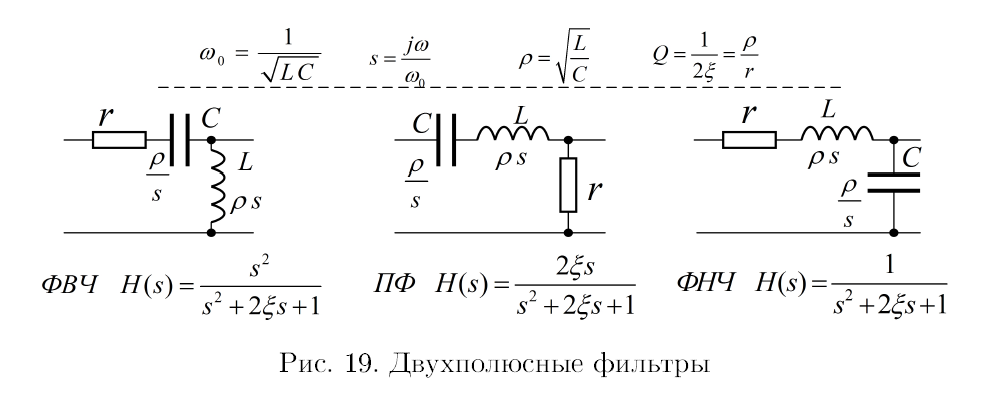
\includegraphics[width=1\textwidth]{4_2.png}
	\label{fig:boiler}
\end{figure}

Комплексный коэффициент передачи ПФ выражается через обобщенную расстройку: $a(\omega)=Q\left(\frac{\omega}{\omega_0}-\frac{\omega_0}{\omega}\right)$
$$
K(j \omega)=\frac{1}{1+\frac{1}{2 \xi}\left(s+\frac{1}{s}\right)}=\frac{1}{1+j a(\omega)}=\frac{1}{\sqrt{1+a^2(\omega)}} e^{-j \operatorname{arctg} a(\omega)} .
$$
У коэффициента передачи ФВЧ присутствует дополнительный множитель $s=\frac{j \omega}{\omega_0}$ в числителе, у ФНЧ - такой же множитель в знаменателе. В окрестности резонанса, при $\omega \simeq \omega_0$, модули этих множителей малосущественны. Однако они дают существенные вклады $\pm \frac{\pi}{2}$ в фазовые характеристики.

Комплексные полюсы проявляют себя колебательными процессами («звоном») на переходных характеристиках:
$$
\begin{array}{cl}
\text { ФВЧ : } & h_0(u)=\frac{e^{-\xi u}}{\eta}\{\eta \cos \eta u-\xi \sin \eta u\} ; \\
\text { ПФ : } & h_0(u)=\frac{e^{-\xi u}}{\eta} \sin \eta u ; \\
\text { ФНЧ : } & h_0(u)=\theta(u)-\frac{e^{-\xi u}}{\eta}\{\eta \cos \eta u+\xi \sin \eta u\}, \\
\text { где } u=\omega_0 t, \eta=\sqrt{1-\xi^2}, 2 \xi=\frac{1}{Q} .
\end{array}
$$

\subsubsection{Выполнение}

\begin{figure}[!h]
	\centering
	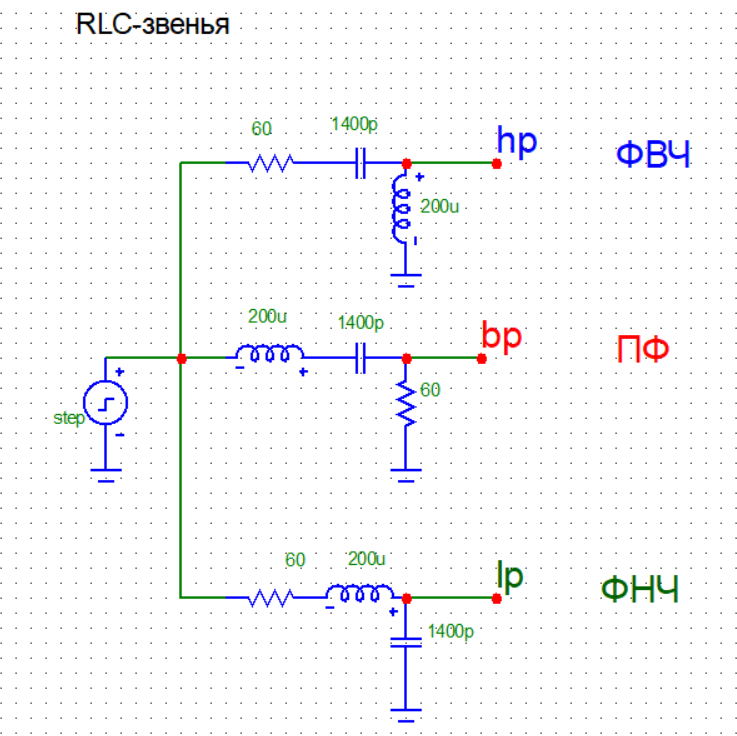
\includegraphics[width=1\textwidth]{4_3.png}
	\label{fig:boiler}
\end{figure}

1) На макетной плате соберем схему полосового фильтра (его схема, как и схема ФНЧ и ФВЧ представлены на рисунке).

\begin{center}
	L = 220 мкГн
	
	C = 1 мкФ
	
	R = 91 Ом
\end{center}

Измерим резонансную частоту и коэффициент передачи

\begin{center}
	$f_0$ = 364 кГц
	
	$f_{min}$ = 298 кГц
	
	$f_{max}$ = 443 кГц
	
	$\Delta f = \frac{f_{max} - f_{min}}{2}$ = 73 кГц
	
	$K(f_0) = \frac{1.947}{4} = 0.4867$
	
	$Q = \frac{\Delta f}{f}$ = 5.0
\end{center}

2) Из тех же компонент соберем схемы ФВЧ и ФНЧ. Измерим для них резонансную частоту и отношения $K(f_0)/K(0)$ для ФНЧ и $K(f_0)/K(\infty)$ для ФВЧ.

\[Q = \frac{K(f_0)}{K(0)} = 5.18\]

\[Q = \frac{K(f_0)}{K(\infty)} = 4.1\]

3) Подключим генератор прямоугольных импульсов. Изучим переходные характеристики ФВЧ, ФНЧ и ПФ. Найдем по осцилограммам период колебаний и время их затухания до уровня $\frac{1}{e}$ и дадим оценку резонансной частоты и добротности.

Для ФВЧ:

\[T = 2.8 \: \text{мкс}\]

\[\tau = 0.45 \: \text{мкс}\]

\[f_0 = 365 \: \text{кГц}\]

\[Q = 6.2\]

Для ФНЧ:

\[T = 2.83 \: \text{мкс}\]

\[\tau = 0.49 \: \text{мкс}\]

\[f_0 = 352 \: \text{кГц}\]

\[Q = 5.7\]

Для ПФ:

\[T = 2.84 \: \text{мкс}\]

\[\tau = 0.51 \: \text{мкс}\]

\[f_0 = 351 \: \text{кГц}\]

\[Q = 5.6\]

4) Для модели rlc2pole изучим частотные фазовые и переходные характеристики фильтров

\begin{figure}[!h]
	\centering
	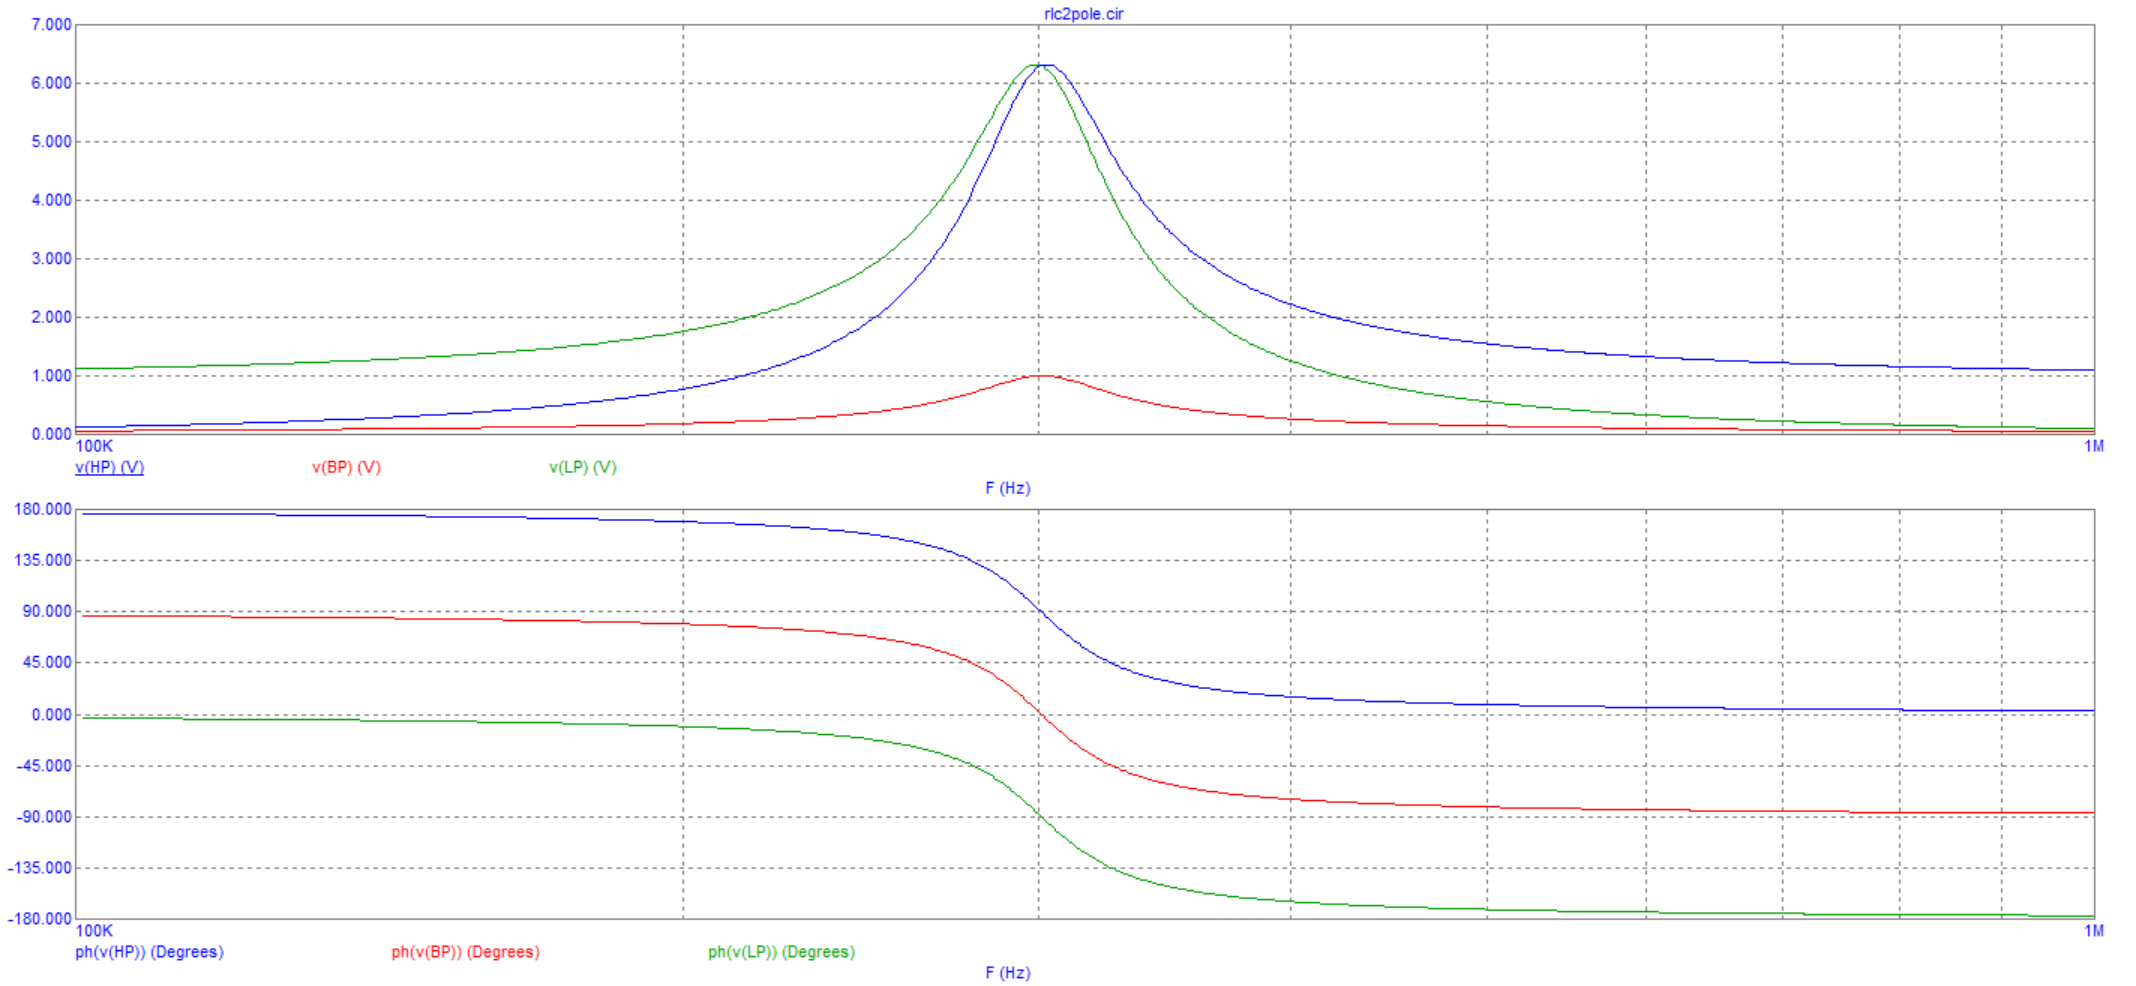
\includegraphics[width=1\textwidth]{4_4.png}
	\label{fig:boiler}
\end{figure}

\begin{figure}[!h]
	\centering
	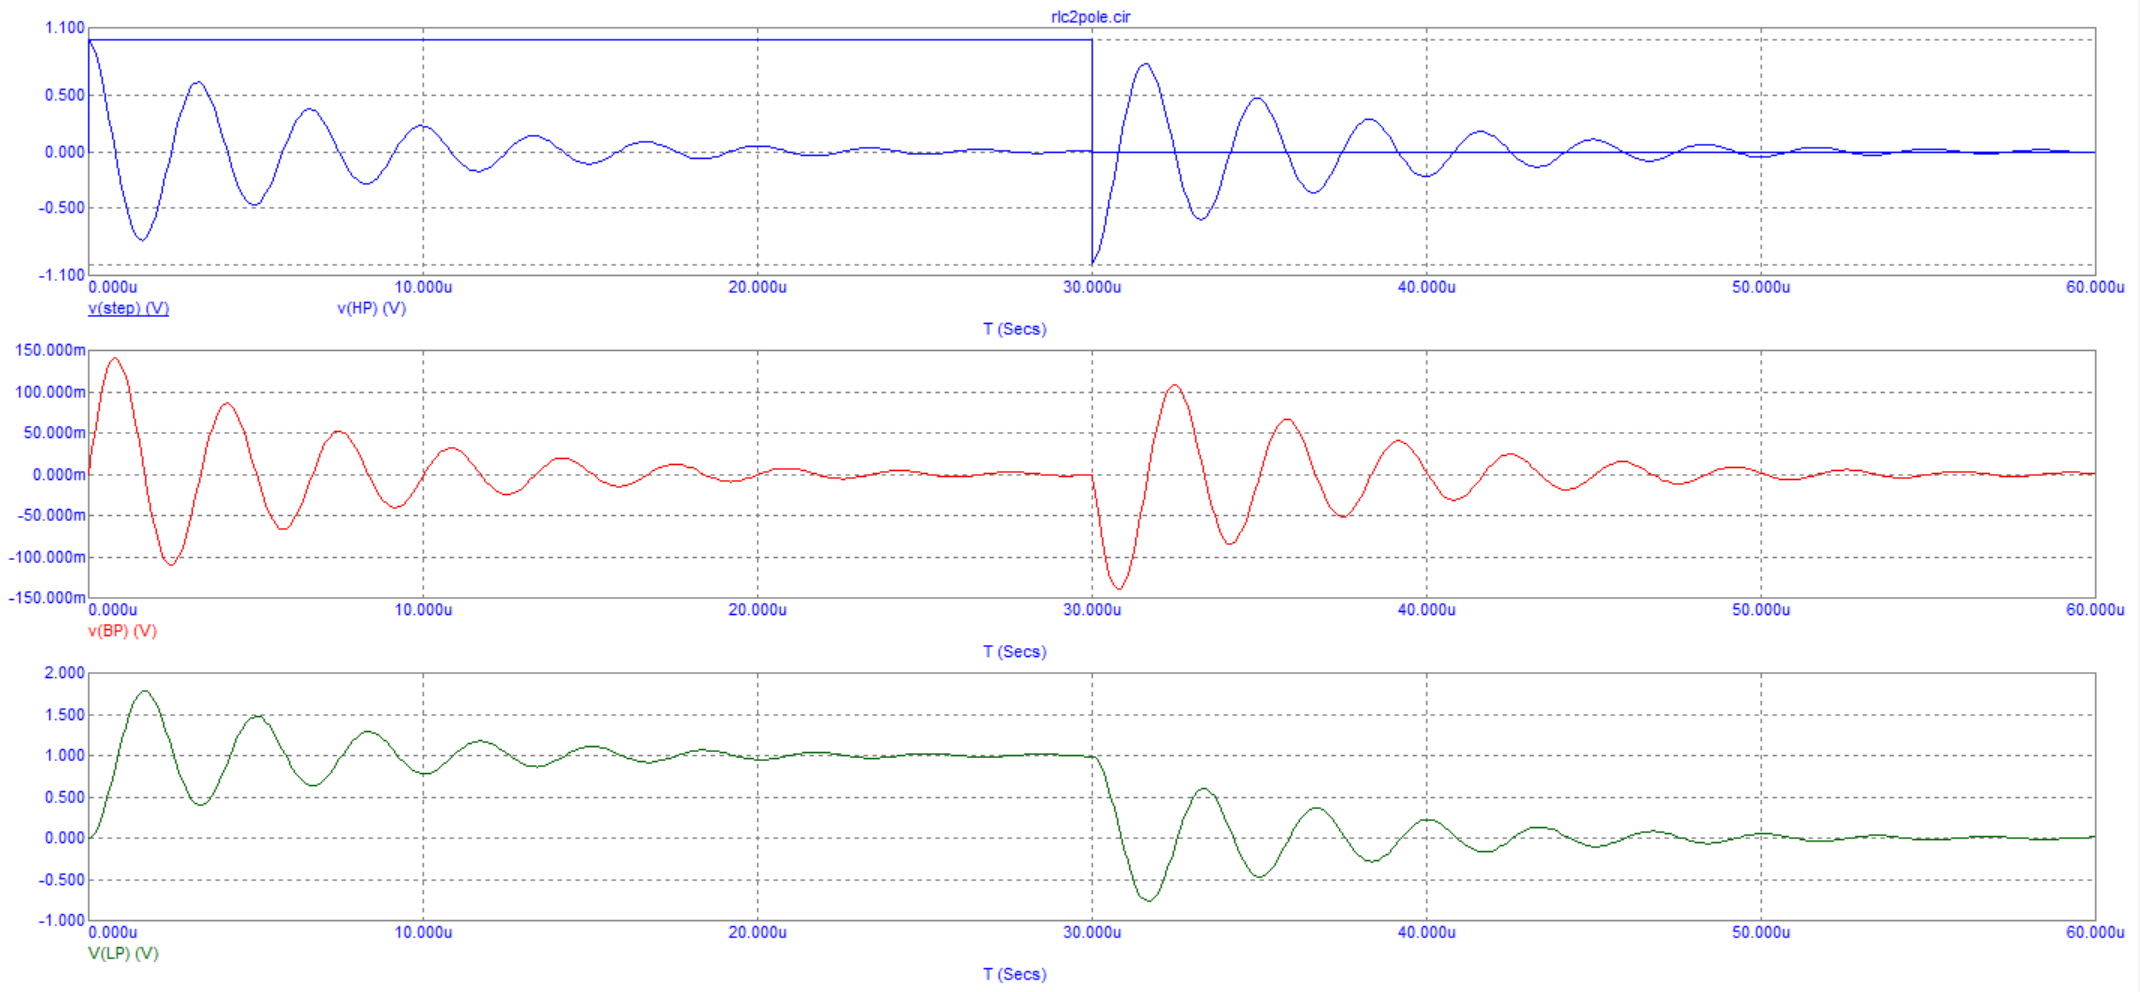
\includegraphics[width=1\textwidth]{4_5.png}
	\label{fig:boiler}
\end{figure}

Собственно говоря, на фчх и ачх видна сама суть фильтров - отсеивать верхние, нижние частоты и диапазон, а на переходной отображены затухающие колебания.

5) Откроем модель groupdel.cir полосового фильтра. Наблюдая в режиме Transient отклик на двухчастотный сигнал изучим зависимость групповой задержки $\tau_g$ от $R = 10, 20, 40, 100$.

\begin{center}
\begin{tabular}{|c|c|c|c|c|}
\hline 
$R, \: \text{Ом}$ & 10 & 20 & 40 & 100 \\ 
\hline 
$\tau_g, \: \text{мс}$ & 0.5 & 0.29 & 0.152 & 0.064 \\ 
\hline 
$\tau_{\textit{теор}}, \: \text{мс}$ & 0.62 & 0.31 & 0.155 & 0.06 \\ 
\hline 
Q & 195 & 98 & 49 & 19 \\ 
\hline 
\end{tabular}
\end{center}

6) Откроем модель lcpower.cir.

\begin{figure}[h!]
\centering
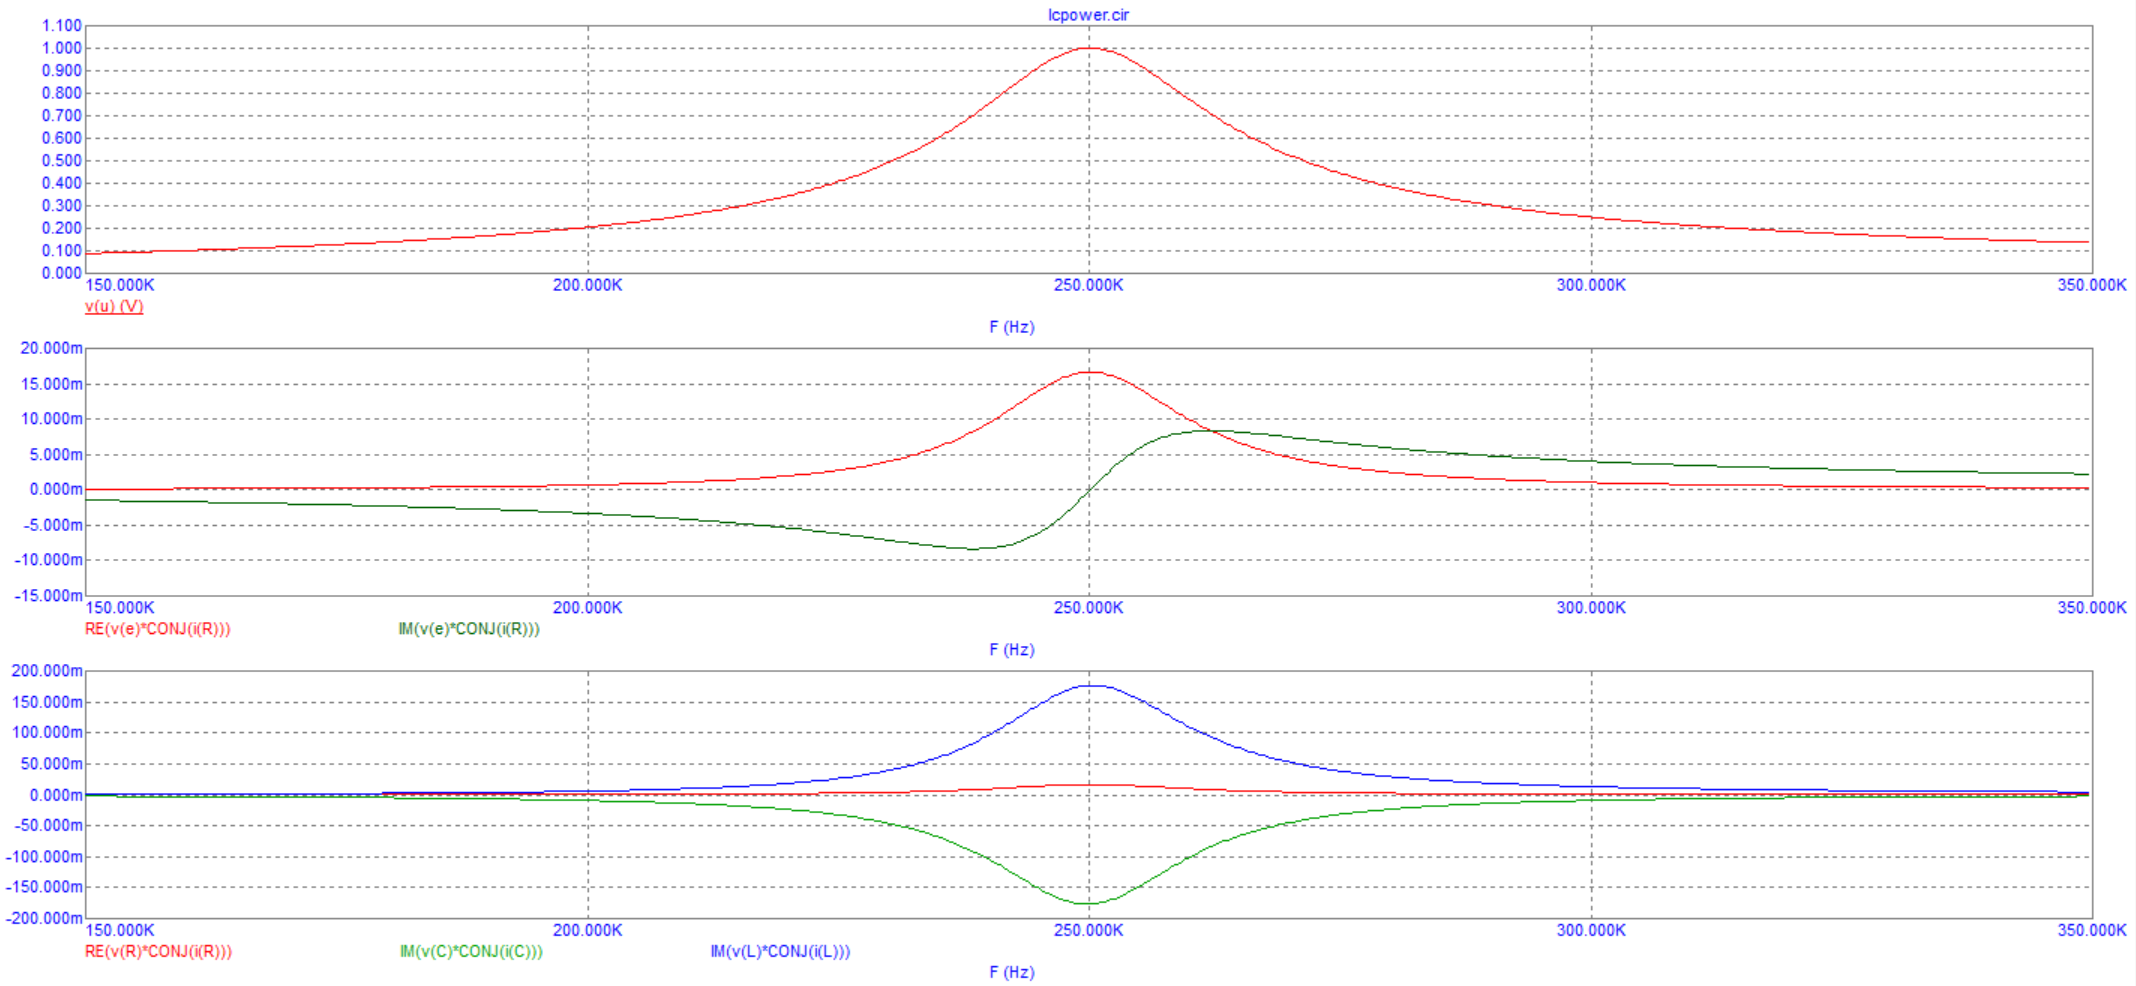
\includegraphics[scale=0.4]{lcpower.png}
\label{fig:Image1}
\end{figure} 

На частоте резонанса $f_0 = 250 \: \text{кГц}$.

\[P_L = 174.468 \: m \quad P_C = -174.468 \: m \quad P_R = 16.71 \: m \Rightarrow \sum P = 16.71 m\]

\[P_{\sum \text{теор}} = 16.7 \: m\]

На одной из границ полосы пропускания $f_1 = 238 \: \text{кГц}$:

\[P_L = 96.484 \: m \quad P_C = -94.331 \: m \quad P_R = 9.567 \: m \Rightarrow \sum P = 9.81 m\]

\[P_{\sum \text{теор}} = 9.8 \: m\]

Закон суммирования выполняется.

\subsubsection{Вывод}

Теория хорошо согласуется с моделированием, практическая работа же согласуется как с результатами моделирования, так и с теоретическими выкладками.

\subsection{Параллельный резонанс}

\subsubsection{Теория}

Параллельный резонанс - это явление, двойственное последовательному. Он наблюдается, когда взаимно уничтожаются мнимые части проводимостей двух параллельных ветвей, рис. 20a. Полная проводимость оказывается при этом вещественной $Y_1 + Y_2 = \frac{1}{R}$, а одинаковые модули мнимых частей проводимостей определяют характеристическое сопротивление $\frac{1}{\rho} = Im(Y_1) = Im(Y_2)$. Параллельный резонанс ярко выражен при большой добротности $Q = \frac{R}{\rho}$, когда резонансное сопротивление значительно превышает характеристическое.

\begin{figure}[!h]
	\centering
	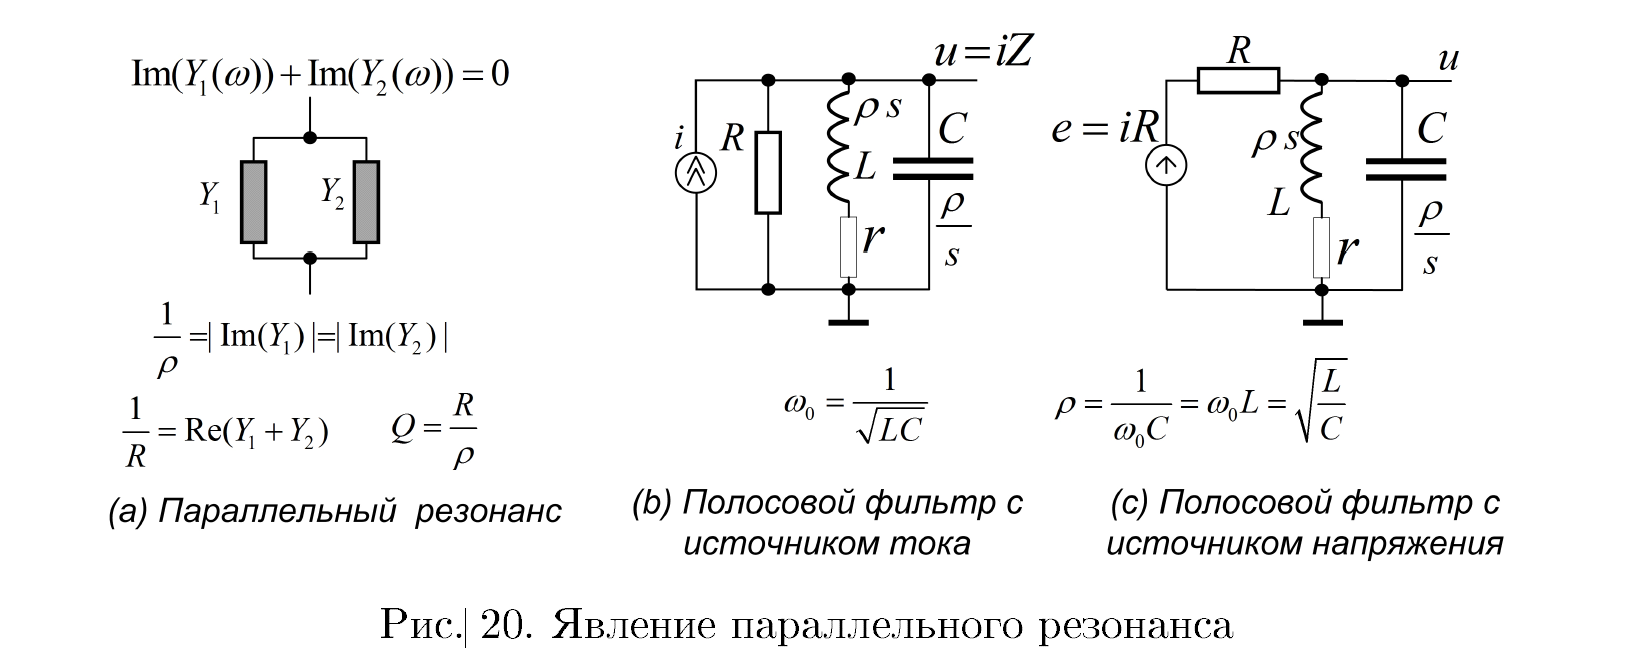
\includegraphics[width=1\textwidth]{5_1.png}
	\label{fig:boiler}
\end{figure}

Два эквивалентных варианта схемы полосового фильтра с параллельным колебательным контуром показаны на рис. 20p,c.
Канонический вариант реализуется в отсутствие последовательных потерь, когда $r=0$. Тогда параллельный резонанс достигается точно на частоте $\omega_0=\frac{1}{\sqrt{L C}}$, а передаточная функция $H(s)=\frac{u}{i}$ (импеданс контура $\left.Z(s)\right)$ принимает вид, обычный для полосовых фильтров второго порядка:
$$
H(s)=Z(s)=\frac{u}{i}=\frac{1}{\frac{1}{R}+\frac{1}{\rho}\left(s+\frac{1}{s}\right)}=\frac{\varrho s}{s^2+2 \xi s+1}=\frac{Q \varrho}{1+j a(\omega)},
$$
где $2 \xi=\frac{1}{Q}=\frac{\rho}{R}$, а $a(\omega)=Q\left(\frac{\omega_0}{\omega}-\frac{\omega}{\omega_0}\right)$ обобщенная расстройка. Сопротив.ление $Q \rho$ контура на частоте резонанса вещественно и превышает его характеристическое сопротивление $\rho$ в $Q$ раз. Передаточная функция схемы с источником напряжения отличается делением на $R: H(s)=\frac{u}{e}=\frac{u}{i R}=\frac{Z(s)}{R}$.

Учет последовательных потерь $r$ усложняет ситуацию. Причин две. Первая связана с тем, что при $r \neq 0$ частота параллельного резонанса, строго говоря, отличается от $\omega_0=\frac{1}{\sqrt{L C}}$. Вторая
38
состоит в том, что при наличии потерь $r$ сопротивление конура на нулевой частоте оказывается ненулевым - равным $r \| R$.

Точное выражение для импеданса контура с последовательными потерями имеет вид
$$
Z(s)=\frac{u}{i}=\frac{\varrho(s+\beta)}{s^2+2 \xi s+1+\alpha \beta} ; \quad \alpha=\frac{\rho}{R}, \beta=\frac{r}{\rho}, 2 \xi=\alpha+\beta .
$$
Полное затухание $2 \xi=\frac{1}{Q}$ равно сумме вкладов $\alpha=\frac{\rho}{R}$ и $\beta=\frac{r}{\rho}$, вносимых последовательными и параллельными потерями. При $r R=\rho^2$ эти вклады одинаковы. Это дает хорошо известный рецепт пересчета последовательных потерь в эквивалентные параллельные: $R=\frac{\rho^2}{r}$.

Ненулевое значение $r$ вызывает сдвиг нуля передаточной функции из нуля в точку $s=-\beta$. В окрестности резонанса влияние этого эффекта почти незаметно. Однако на малых частотах поведение системы меняется радикально - нуль проявляет себя нарастанием фазового сдвига от нуля на нулевой частоте до $+\frac{\pi}{2}$.

Последовательные потери $r$ приводят к сдвигу частоты параллельного резонанса по закону $\omega=\omega_0 \sqrt{1-\beta^2}$. Этот эффект ощутимо сказывается на частоте пересечения нуля фазовой характеристикой.

\subsubsection{Выполнение}

\newpage

1) Откроем в MicroCap модель parallel.cir параллельного контура с $f_0 = 100 \: \text{кГц}$, $\varrho = 570$. По схеме оценим параметры:

\[\alpha = \frac{\rho}{R_0}\]

\[\beta = \frac{R}{\rho}\]

\[Q = \frac{1}{\alpha + \beta}\]

\begin{figure}[!h]
	\centering
	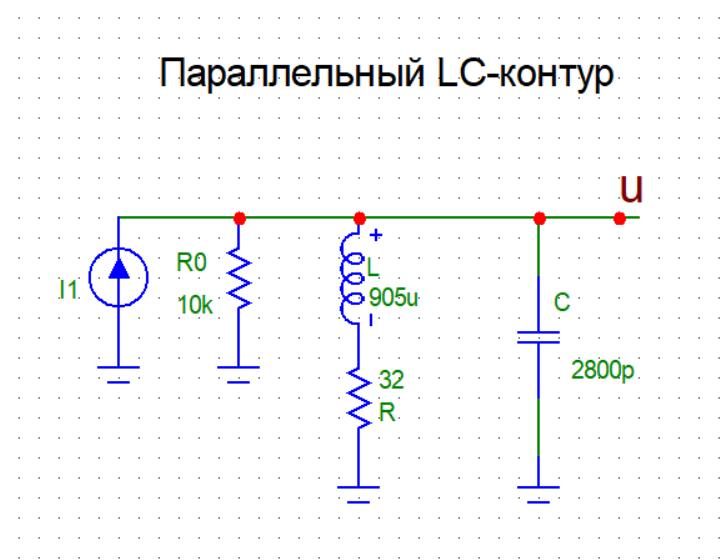
\includegraphics[width=1\textwidth]{5_2.png}
	\label{fig:boiler}
\end{figure}

\[\rho = \sqrt{\frac{L}{C}} = 568\]

\[\alpha = 0.0568 \quad \beta = 0.0563\]

\[Q = 8.84\]

2) Резонансная частота $f_0 = 100 \: \text{кГц}$, полосу пропускания $\Delta f = 11.6 \: \text{кГц}$. Измерим сопротивление контура $R_0 = 5 \: \text{кОм}$ (Напряжение в резонансе деленное на ток 1 ампер). Оценим добротность как:

\[Q = \frac{R_0}{\rho} = 8.8\]

\[Q = \frac{f_0}{\triangle f} = 8.6\]

3) Изучим влияние на добротность последовательных потерь \textit{R}, установив варьирование $R = [0, 32 \Vert 32]$. 

\begin{figure}[h!]
\centering
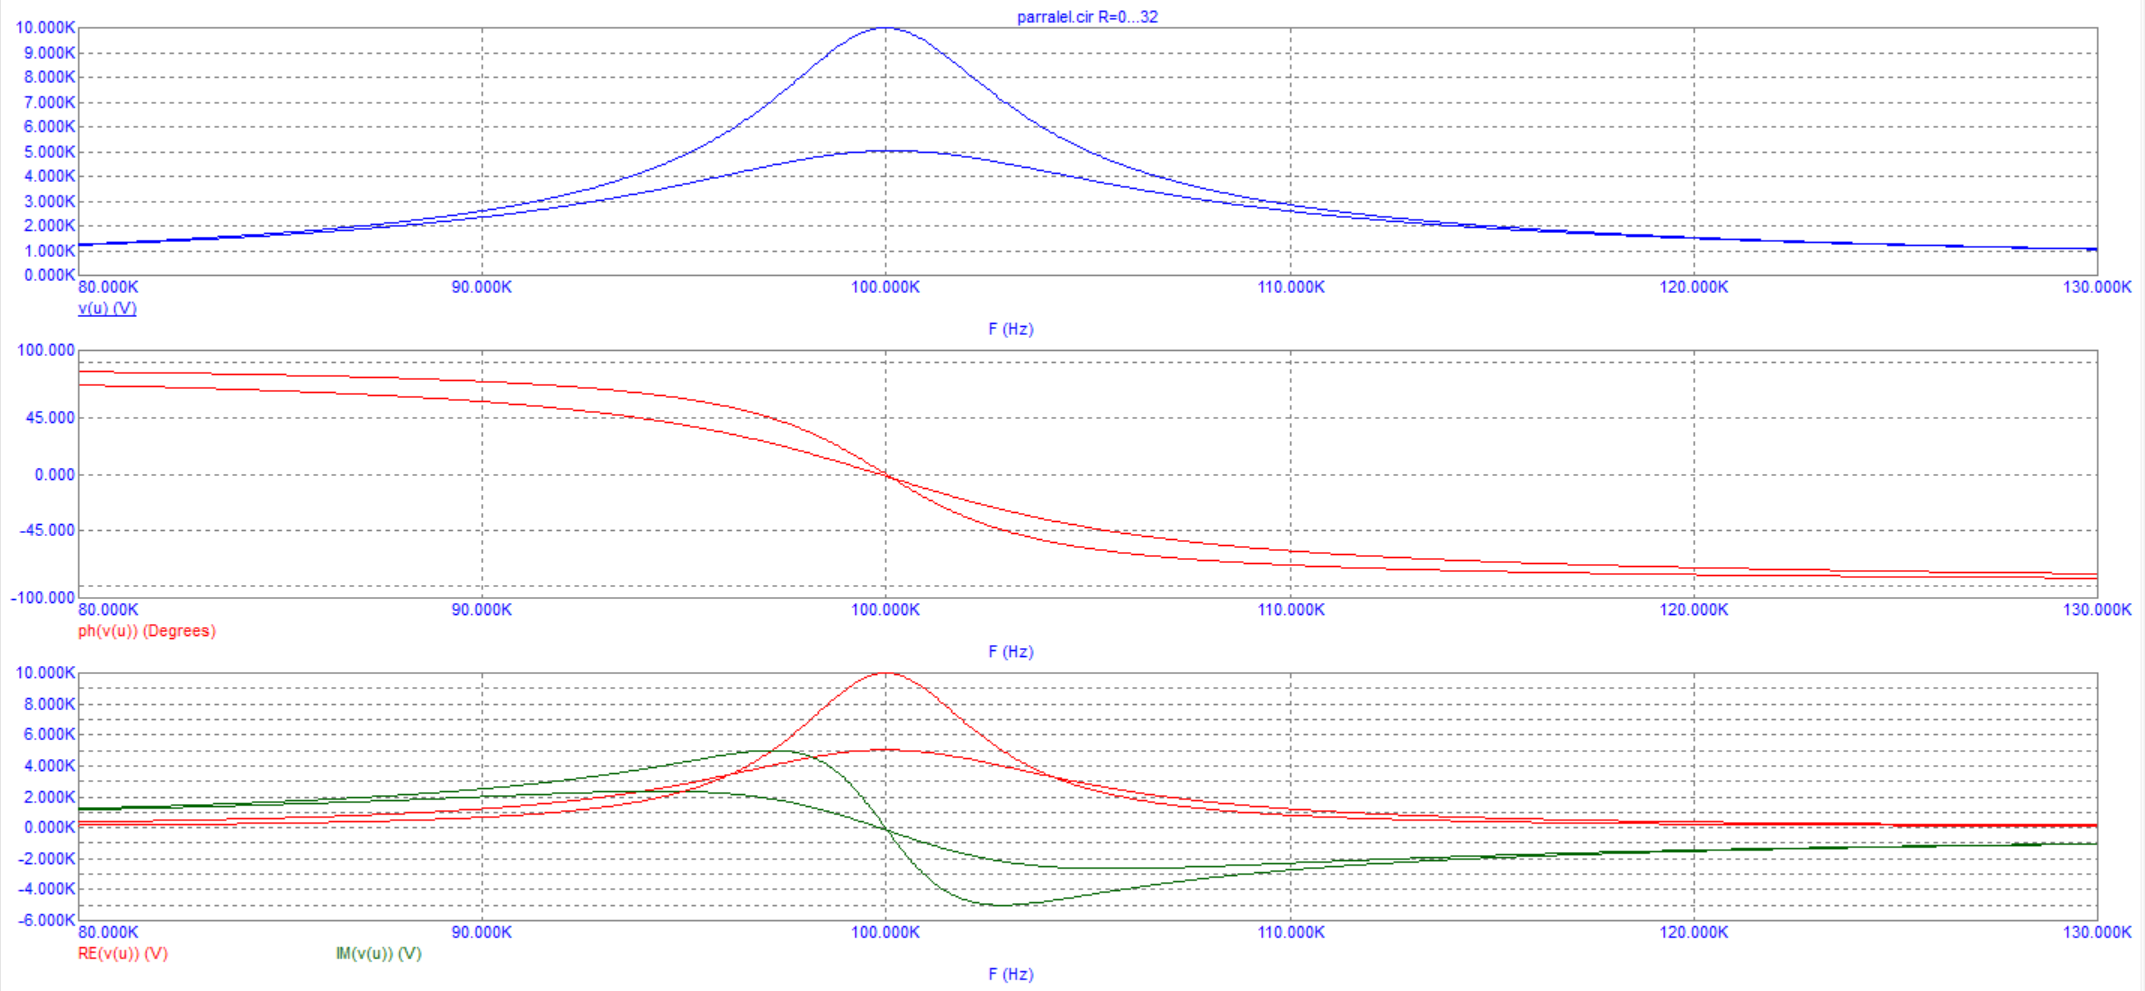
\includegraphics[scale=0.4]{parallel_AC1.png}
\label{fig:Image1}
\end{figure} 

Добротность при $R = 0$:

\[Q = \frac{f_0}{\triangle f} = 17.3\]

Изучим влияние параллельных потерь $R_0$, установив варьирование $R_0 = [10k, 1000k \Vert 1000k]$. Измерим добротность при $R_0 = 1000 \: \text{кОм}$:

\[Q = \frac{f_0}{\Delta f} = 17.2\]

При увеличении $R$ от 0 \textit{Ом} до 32 \text{Ом} $1/Q$ меняется от 0.058 до 0.116. При увеличении $R_0$ от 10 \text{кОм} до 1000 \text{кОм} $1/Q$ меняется от 0.116 до 0.058.

\newpage

4) Изучим зависимость частоты параллельного резонанса от $R = [0, 150 \Vert 50]$.

\begin{figure}[h!]
\centering
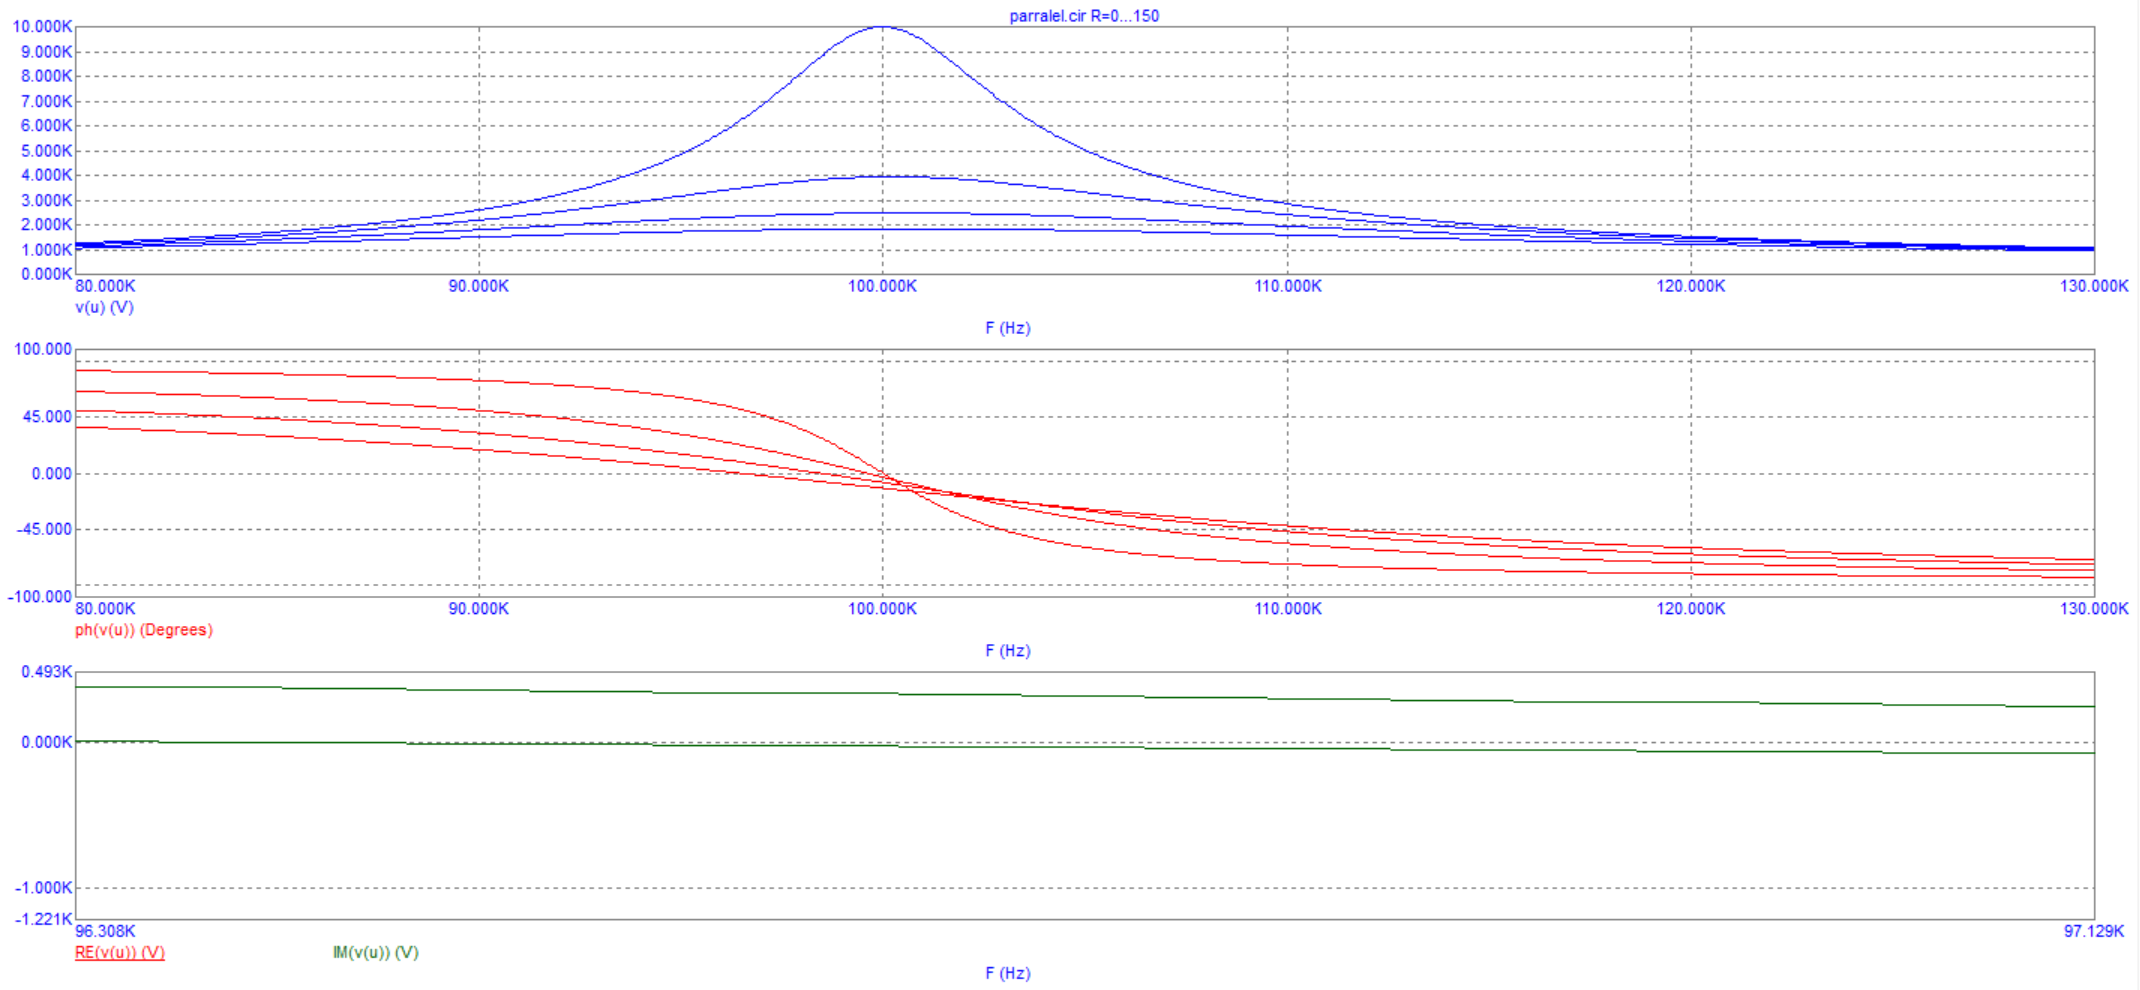
\includegraphics[scale=0.4]{parallel_AC2.png}
\label{fig:Image1}
\end{figure} 

\begin{center}
\begin{tabular}{|c|c|c|c|c|}
\hline 
$R, \: \text{Ом}$ & 0 & 50 & 100 & 150 \\ 
\hline 
$f_{\text{эксп}}, \: \text{кГц}$ & 100 & 99.6 & 98.42 & 96.4 \\ 
\hline 
$\beta$ & 0 & 0.088 & 0.176 & 0.264 \\ 
\hline 
$f_{\text{теор}}$ & 100 & 99.6 & 98.43 & 96.45 \\ 
\hline 
\end{tabular} 
\end{center}

5) Исследуем влияние последовательных потерь в области низких частот. Установим частотный диапазон от $1 \: \text{кГц}$ до $130 \: \text{кГц}$ и будем варьировать $R = [0,20 \Vert 2]$.

\begin{figure}[h!]
\centering
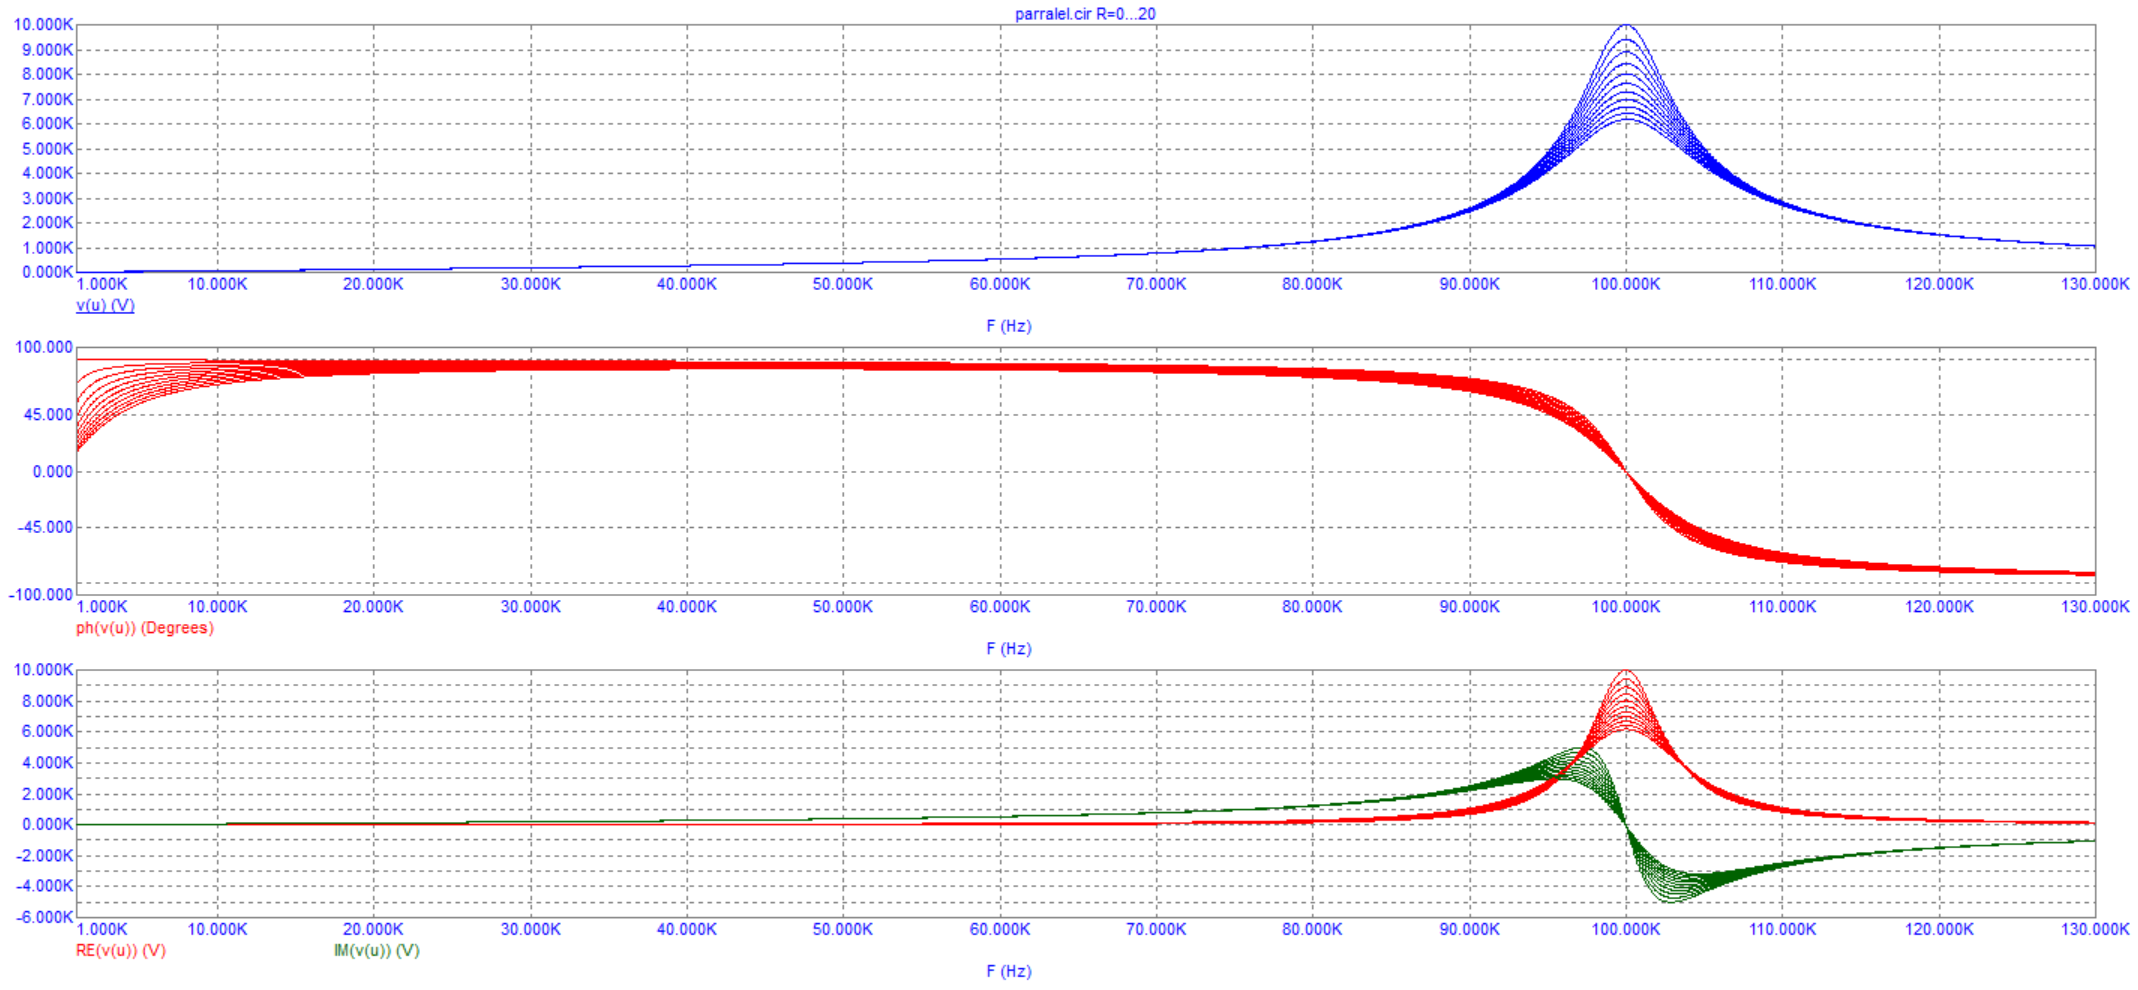
\includegraphics[scale=0.4]{parallel_AC3.png}
\label{fig:Image1}
\end{figure} 

Получаем, что при $R = 12 \: \textit{Ом}$ фазовый сдвиг на частоте $f = 2 \: \textit{кГц}$ составляет $\pi / 4$. 

\subsubsection{Вывод}

Результаты моделирования и теории совпадают.

\subsection{Смешанные резонансы}

\subsubsection{Теория}

В сложной RLC-схеме может наблюдаться сразу несколько
последовательных и параллельных резонансов. Простой пример
такого смешанного резонанса дает контур на рис. 22.

\begin{figure}[!h]
	\centering
	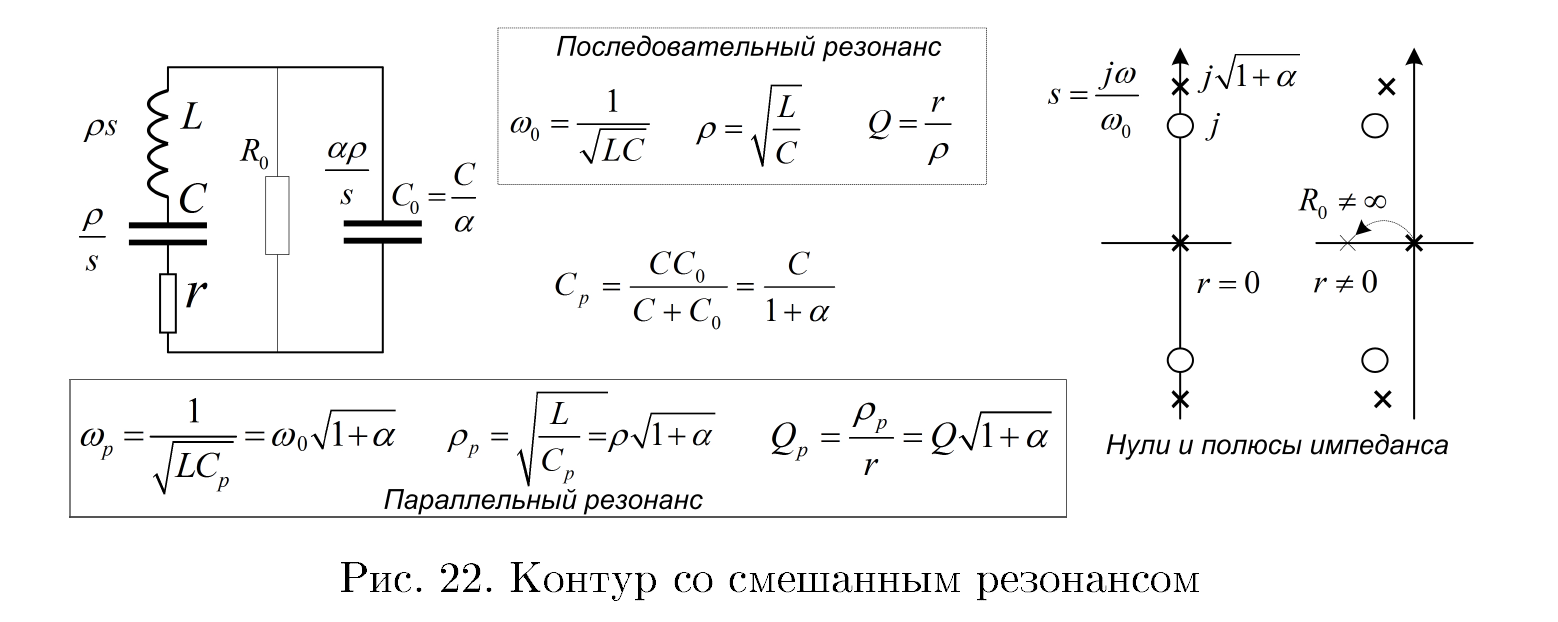
\includegraphics[width=1\textwidth]{6_1.png}
	\label{fig:boiler}
\end{figure}

В его левой LC-ветви присутстует последовательный резонанс на частоте $\omega_0=\frac{1}{\sqrt{L C}}$ а параллельное соединение двух ветвей дает параллельный резонанс на частоте $\omega_p=\frac{1}{\sqrt{L C_p}}=\omega_0 \sqrt{1+\alpha}$. Частота параллельного резонанса всегда выше частоты последовательного и приближается к ней при $\alpha \rightarrow 0$.

Без учета параллельных потерь $\left(R_0=\infty\right)$ импеданс этого контура имеет вид
$$
Z(s)=\frac{\alpha \rho}{s} \frac{s^2+2 \xi s+1}{\left(s^2+2 \xi s+1+\alpha\right)}=\frac{\alpha \rho}{s} \frac{1+j a(\omega)}{\left(1+j a_p(\omega)\right)},
$$
где $s=\frac{j \omega}{\omega_0}, 2 \xi=\frac{r}{\rho}=\frac{1}{Q}$, :
$$
a(\omega)=Q\left(\frac{\omega}{\omega_0}-\frac{\omega_0}{\omega}\right) ; \quad a_p(\omega)=Q_p\left(\frac{\omega}{\omega_p}-\frac{\omega_p}{\omega}\right) ; \quad Q_p=Q \sqrt{1+\alpha} .
$$
В отсутствие потерь $(r=0, \xi=0)$, рис. 22 имется полюс в нуле, пара нулей в точках $s= \pm j .\left(\omega=\omega_0\right)$ и пара полюсов при
41
$s= \pm j \sqrt{1+\alpha}\left(\omega=\omega_p=\omega_0 \sqrt{1+\alpha}\right)$. Эти объекты и определяют поведение частотной и фазовой характеристик системы.

Полюе в нуле вносит фазовый слвиг на $-\frac{\pi}{2}$, см. рис. 23 . 1 ри пересечении нуля добавляется слвиг на $+\pi$, а при пересечении полюса такой же сдвиг вычитиется. На интервале между нулем и полюсом - между последовательным и параллельным резонан сами - фазовый сдвиг принимает значение $+\frac{\pi}{2}$, что отвечнет ин дуктивному импедансу. Вне этого интервала импеданс контура оказывнется емкостным.

\begin{figure}[!h]
	\centering
	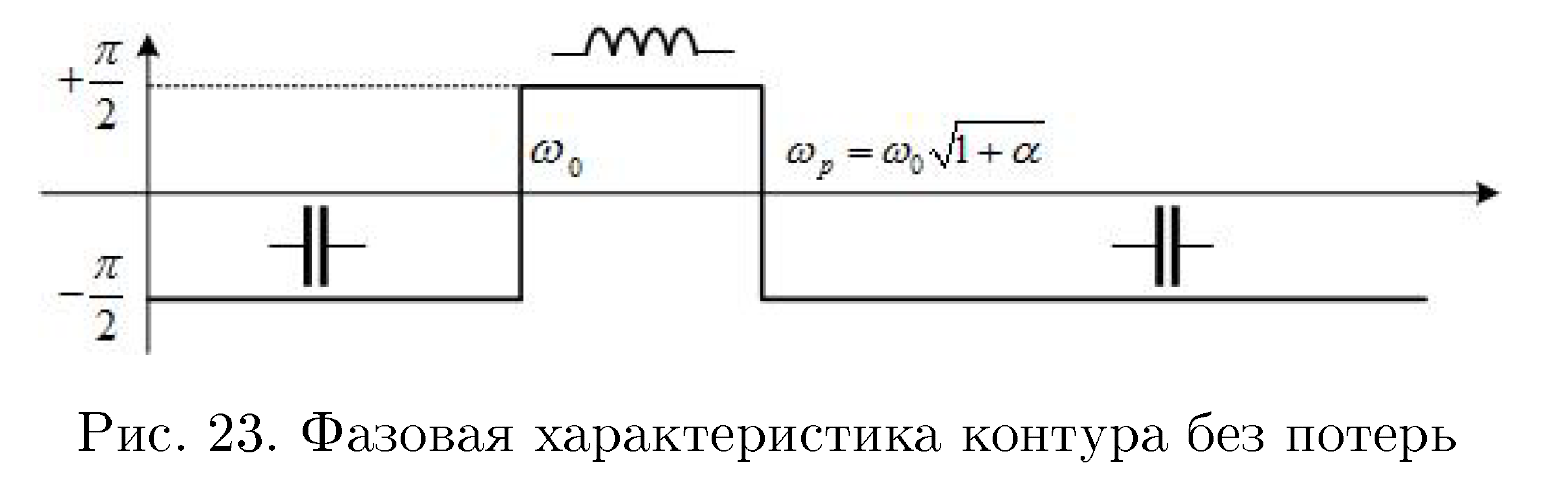
\includegraphics[width=0.7\textwidth]{6_2.png}
	\label{fig:boiler}
\end{figure}

При добавлении потерь $r$ сопряженные нули и полюсы смещағося с мнимой оси в левую $s$ полуплоскость, рис. 22. Фазовая характеристика, не менять по существу, сглаживается, а провал и выброс на частотной характеристике в точках $\omega_0, \omega_p$ становятся конечными:
$$
Z\left(\omega_0\right)=\frac{r}{1+j \frac{1}{\alpha Q}} \simeq r ; \quad Z\left(\omega_p\right)=k^2 Q_p \varrho_p\left(1-j \frac{1}{k Q}\right) \simeq k^2 Q_p \varrho_p,
$$
где $k=\frac{\alpha}{1+\alpha}=\frac{C}{C+C_0}-$ коэффициент подключения контура.

Главный эффект от добавления параллельных потерь $R_0-$ это сдвиг полюса при $s=0$ в ненулевую точку на вещестенной оси, рис, 22. В результате импеданс контура на нулевой частоте стнновится конечным - равным $R_0$. Параллельные потери заметно влияют также и на положение пары сопряженных полюсов, снижая их добротность, но почти не оказывая влияния на положение нулей.

\subsubsection{Выполнение}

1) Откроем модель \text{combined.cir} с $f_0 = 100 \: \text{кГц}$, $\rho = 15.9 \: \text{кГц}$, $q \simeq 10$, $\alpha = 1$.

\begin{figure}[h!]
\centering
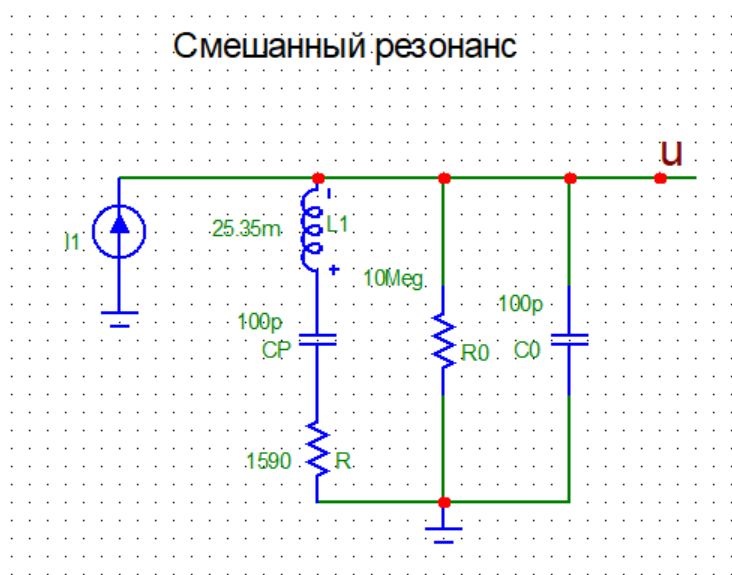
\includegraphics[scale=1]{combined_img.png}
\label{fig:Image1}
\end{figure}

Изучим графики частотной и фазовой характеристик, а также графики частотных зависимостей вещественной и мнимой частей мпеданса.

\begin{figure}[h!]
\centering
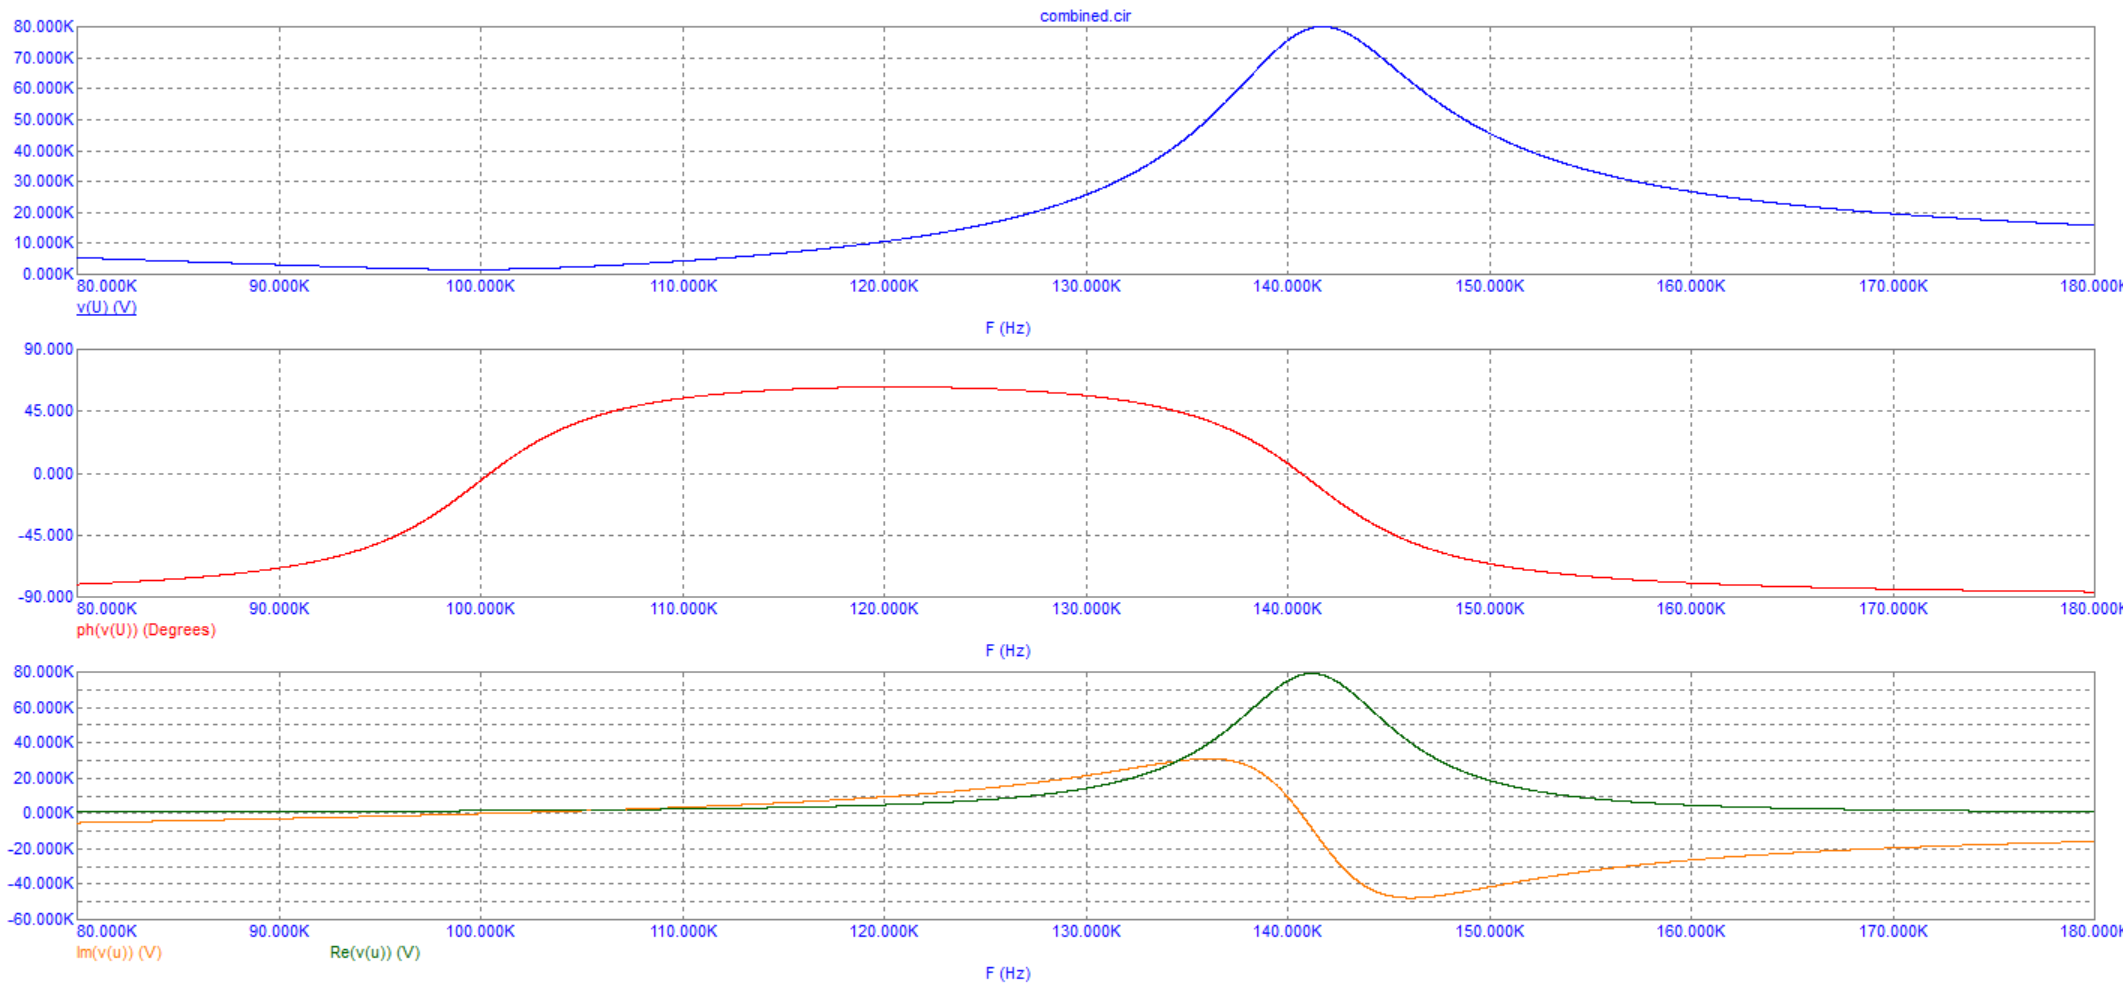
\includegraphics[scale=0.4]{combined_AC1.png}
\label{fig:Image1}
\end{figure}

2) Измерим частоты $f_p, f_0$ последовательного и параллельного резонансов по точкам пересечения нуля фазовой характеристикой:

\[f_p = 100.5 \: \text{кГц} \quad f_0 = 140.6 \: \text{кГц}\]

Измерим полосы $\triangle f_p, \triangle f_0$, в которых фазовая характеристика изменяется в диапазоне $\pm 45 ^\circ$ в окрестностях резонансов.

\[\triangle f_p = 10.6 \: \text{кГц}\]

\[\triangle f_0 = 10.8 \: \text{кГц}\]

Оценим добротности $Q_p, Q_0$ и проверим, что $f_0 = f_p \sqrt{2}$, $Q_0 = Q_p \sqrt{2}$:

\[Q_p = \frac{f_p}{\triangle f_p} = 9.5\]

\[Q_0 = \frac{f_0}{\triangle f_0} = 13\]

\[Q_0 = 13 \simeq 13.43 = Q_p \sqrt{2}\]

\[f_0 = 140.6 \simeq 142,1 = f_p \sqrt{2}\]

3) Измерим сопротивление контура на частотах последовательного и параллельного резонансов, сравним результаты с теоретическими значениями ($r, k^2\rho_p, Q_p$):

\[r_{\text{эксп}} = 1.565 \: \text{кОм} \simeq 1.59 \: \text{кОм} = r_{\text{теор}}\]

\[(k^2\rho_p, Q_p)_{\text{эксп}} = 78.1 \: \text{кОм} \simeq  79.1 \: \text{кОм} = \Big(\frac{\alpha}{1 + \alpha}\Big)^2 \sqrt{\frac{L}{c}}(1 + \alpha)\frac{r}{\rho} = (k^2\rho_p, Q_p)_{\text{теор}}\]

Снимем зависимость сопротивления на частоте параллельного резонанса от $R = [500, 2000 \Vert 500]$ и емкости $C_0 = [100p, 300p \Vert 100p]$. Сопоставим их с теорией. Осмыслим характер изменения графиков при варьировании $R$ и $C_0$.

\begin{figure}[h!]
\centering
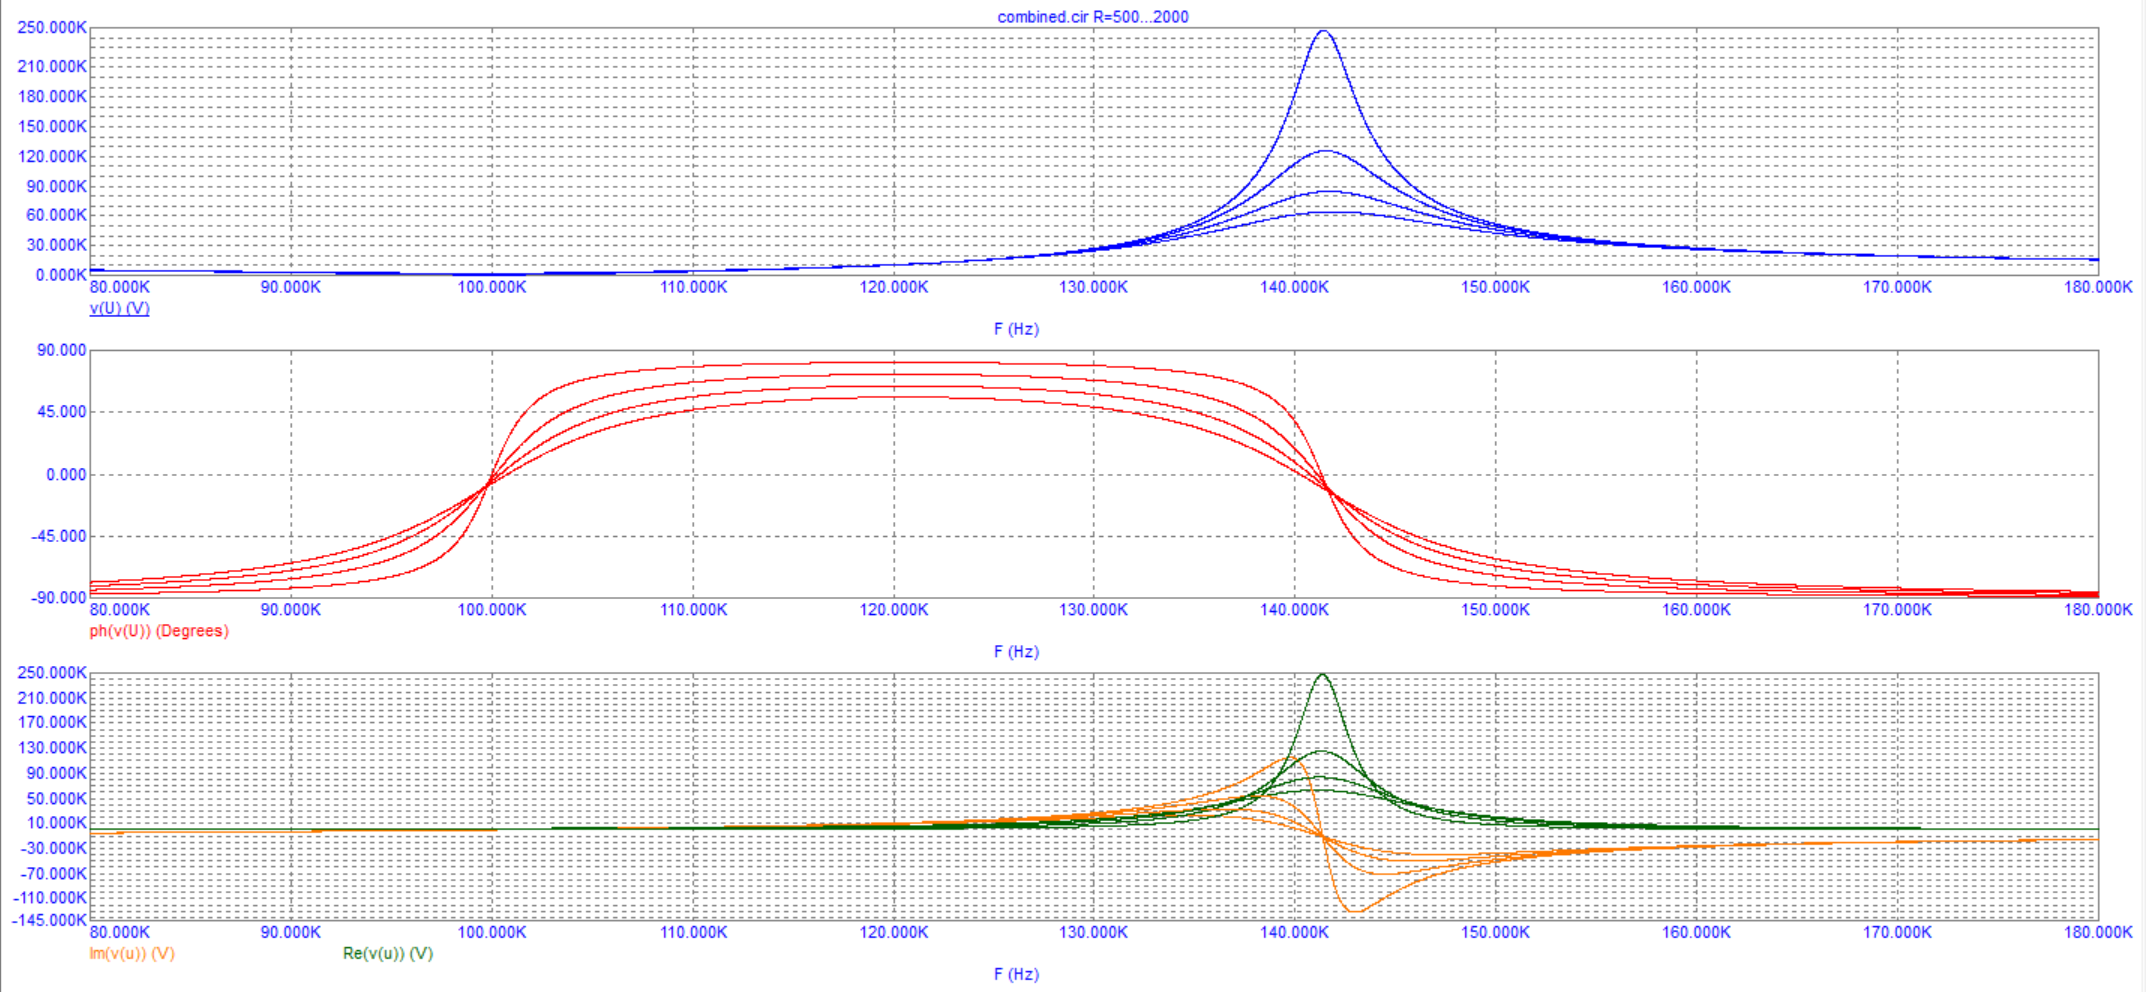
\includegraphics[scale=0.4]{combined_AC2.png}
\label{fig:Image1}
\end{figure}

\begin{center}
\begin{tabular}{|c|c|c|c|c|}
\hline 
$R, \: \text{Ом}$ & 500 & 1000 & 1500 & 2000 \\ 
\hline 
$Z, \: \text{кОм}$ & 247 & 124.4 & 83 & 61.9 \\ 
\hline 
\end{tabular} 
\end{center}

Получаем зависимость:

\[Z \sim \frac{1}{R}\]

\begin{figure}[h!]
\centering
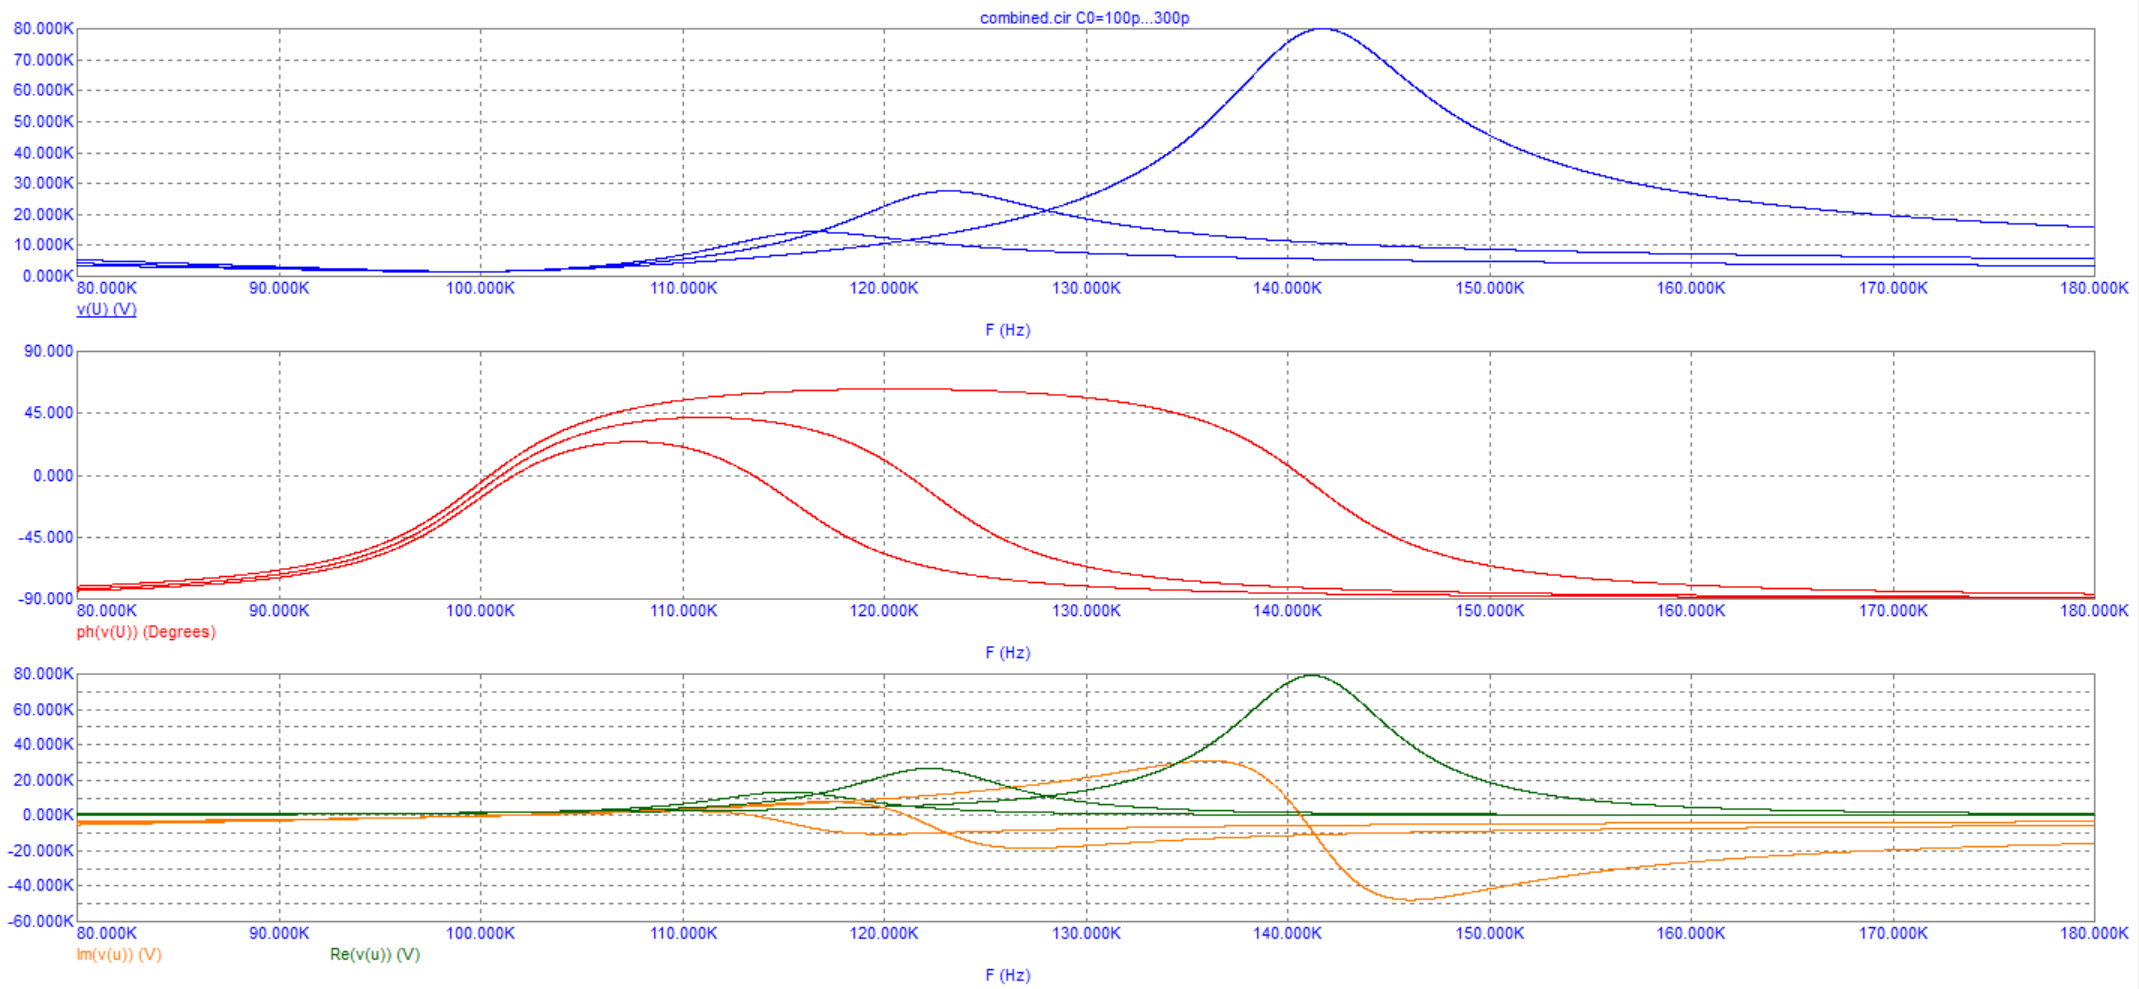
\includegraphics[scale=0.4]{combined_AC3.png}
\label{fig:Image1}
\end{figure}

\begin{center}
\begin{tabular}{|c|c|c|c|}
\hline 
$C_0, \: \text{пФ}$ & 100 & 200 & 300 \\ 
\hline 
$Z, \: \text{кОм}$ & 78.3 & 25.4 & 11.9 \\ 
\hline 
\end{tabular} 
\end{center}

Получаем зависимость:

\[Z \sim \frac{1}{C_0^2}\]

4) Обнулим последовательности потери $r$ и варьированием $R_0 = [10k, 100k \Vert 10k]$ подберем сопротивления параллельных потерь так, чтобы достичь того же резонансного сопротивления, что и при $r = 1590 \: \text{Ом}$.

\begin{figure}[h!]
\centering
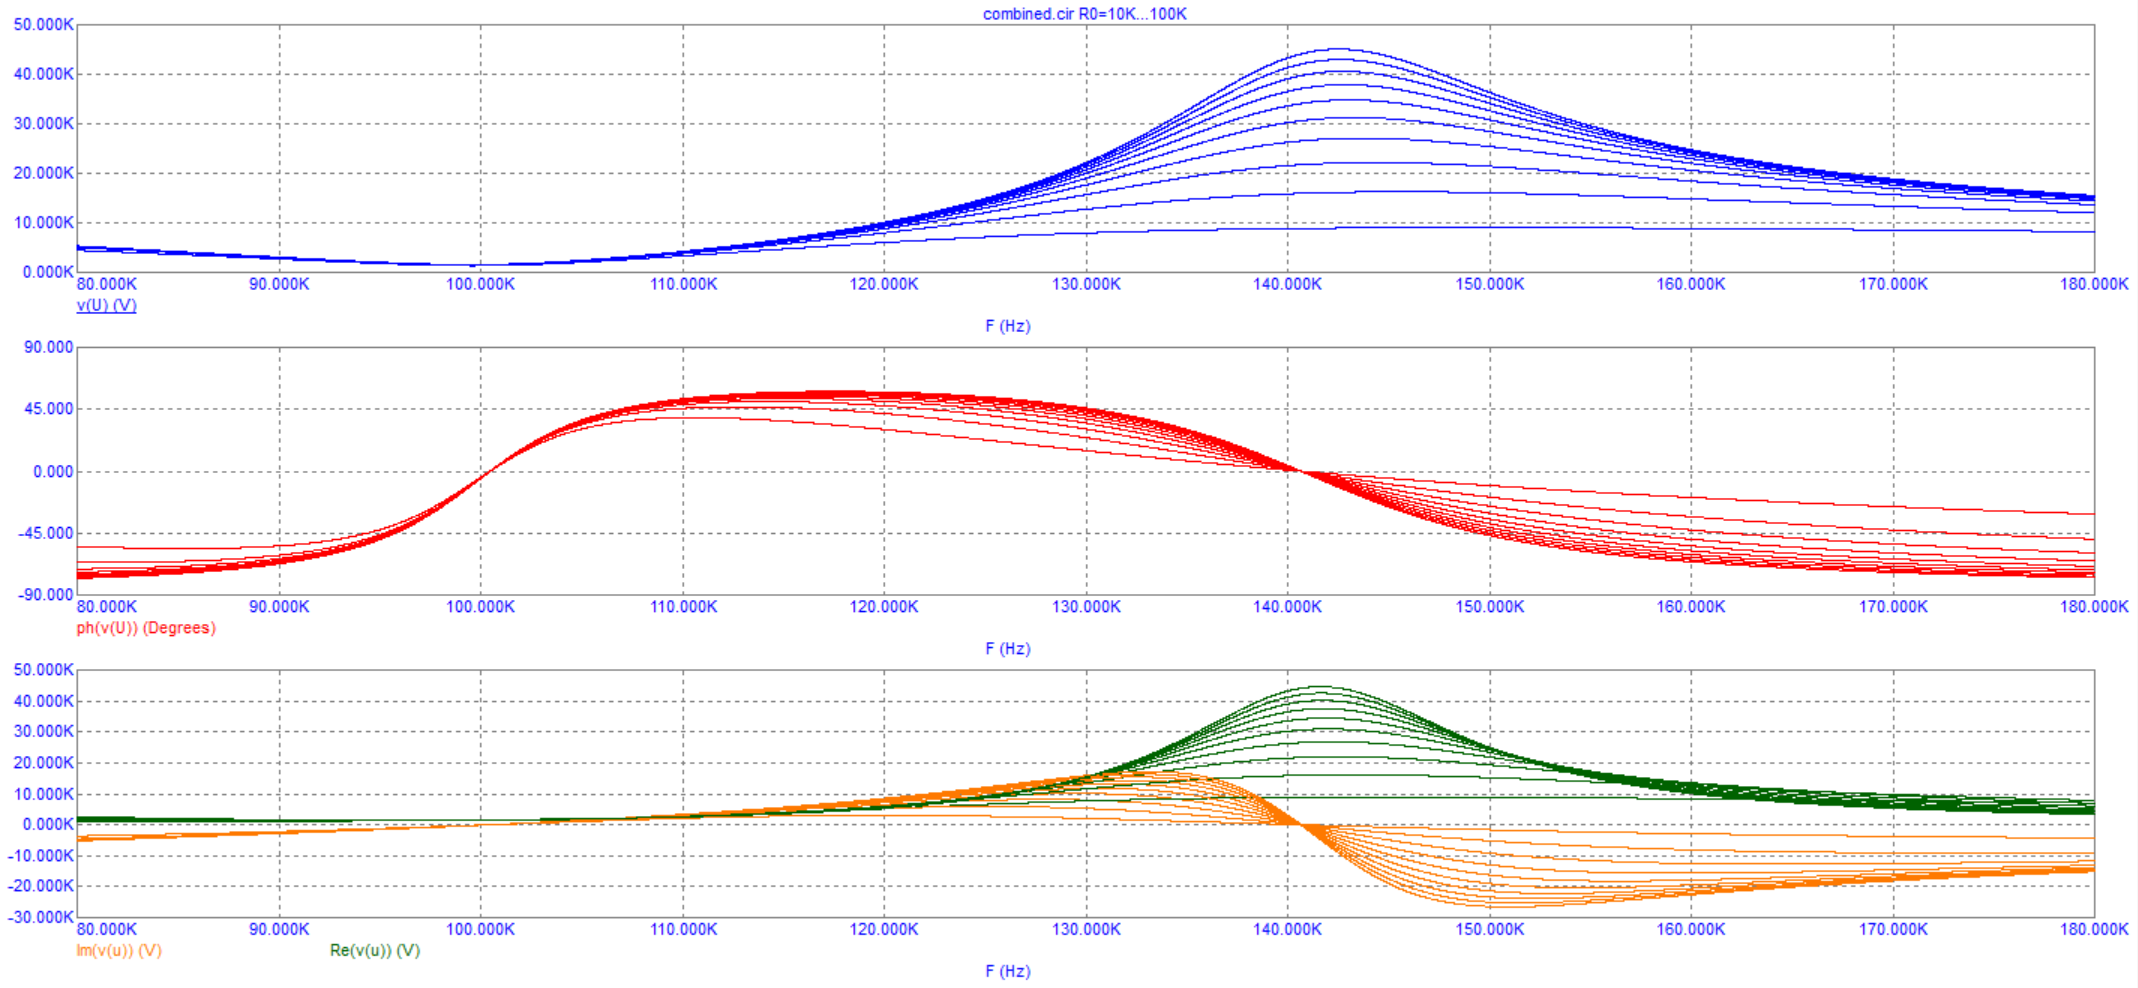
\includegraphics[scale=0.4]{combined_AC4.png}
\label{fig:Image1}
\end{figure}

Получим $R_0 = 80 \: \text{кОм}$. Проверим закон пересчета:

\[R_0 r = k^2 \rho_p^2\]

\[80000 \cdot 1590 \simeq \Big(\frac{1}{2}\Big)^2 \cdot 2 \cdot 15900^2.\]

Соотношение выше выполняется.

5) Варьируя $R_0 = [80k, 10Meg \Vert 10Meg]$ при $r = 1590 \: \text{Ом}$, изучим влияние $R_0$ на поведения частотной и фазовой характеристик на низких частотах - в диапазоне $1k, 180k$.

\begin{figure}[h!]
\centering
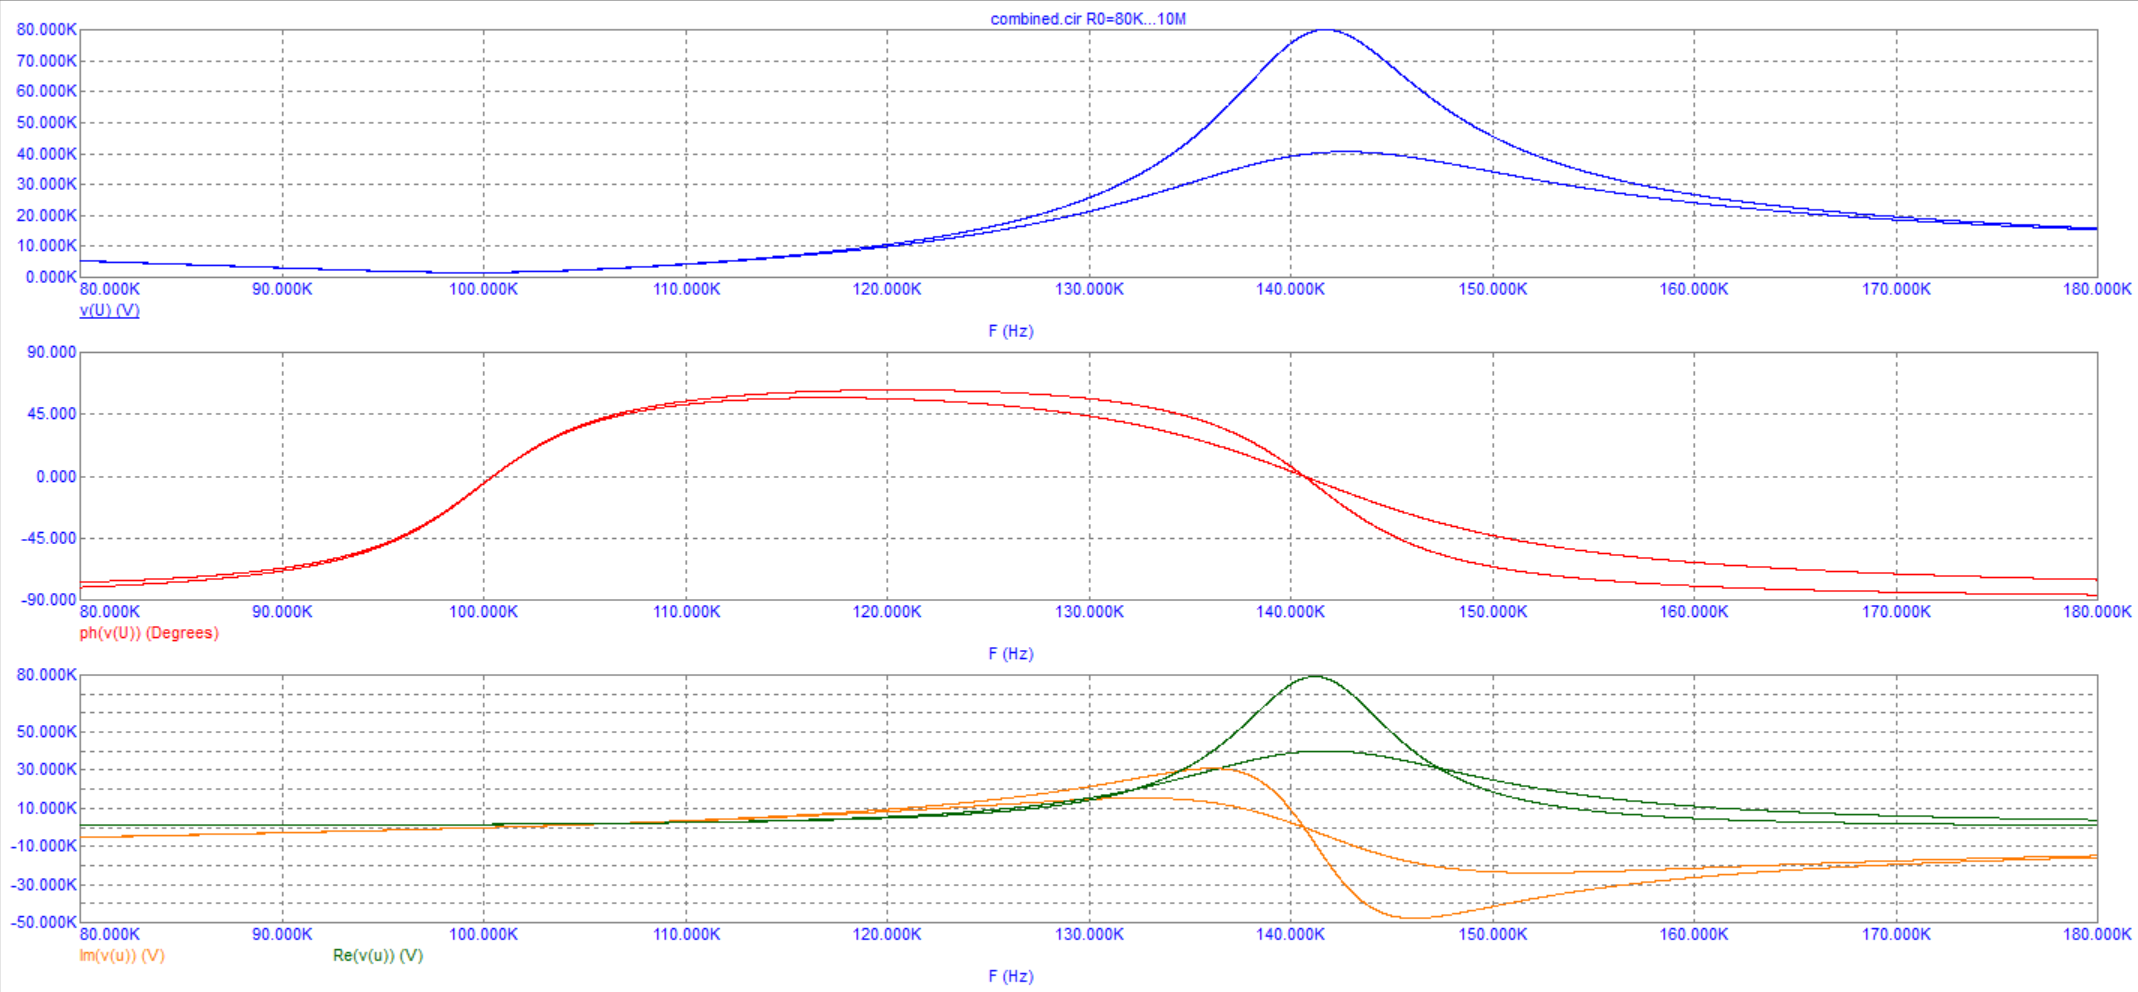
\includegraphics[scale=0.4]{combined_AC5.png}
\label{fig:Image1}
\end{figure}

При увеличении $R_0$ частотная характеристика увеличивается, а фазовая уменьшается.

\subsubsection{Вывод}

Результаты теории согласуются с измерениями.

\section{Вывод}

Результаты моделирования, как и ожидается, тождественны теории, в то время как замеры на макетной плате незначительно от нее отличаются. Все это позволяет сказать, что использованные методы расчета и анализа безинерционных линейных цепей дают хорошие результаты в области применимости.


\end{problem}
\end{document}







